% Retoca las líneas marcadas con TODO según las necesidades

\documentclass[oneside,a4paper,12pt]{book} % TODO: cambia "oneside" por "twoside" a la hora de imprimirlo

\usepackage[spanish]{babel}
\usepackage[utf8]{inputenc}
\usepackage{geometry}
\usepackage{makeidx}
\usepackage{url}
\usepackage{xurl}
\usepackage{graphicx}
\usepackage{color}
\usepackage{caption}
\usepackage{acronym}
\usepackage{hyphenat}
\usepackage{a4wide}
\usepackage[normalsize]{subfigure}
\usepackage{float}
\usepackage{titlesec}
\usepackage[Lenny]{fncychap}
\usepackage{listings} % para poder hacer uso de "listings" propios (p.ej. códigos)
\usepackage{eurosym} % para poder usar el símbolo del euro con \euro {xx}
\usepackage{hyperref} % TODO: añade la opción hidelinks para imprimirlo (los enlaces no aparecerán resaltados)
\usepackage{xspace}
\usepackage{subcaption}
\usepackage{amssymb}
\usepackage{siunitx}
\usepackage{yhmath}
\usepackage{svg}


\usepackage{color}
\definecolor{gray}{rgb}{0.4,0.4,0.4}
\definecolor{darkblue}{rgb}{0.0,0.0,0.6}
\definecolor{cyan}{rgb}{0.0,0.6,0.6}

\sisetup{per-mode=symbol} % Configuración para mostrar la unidad con el símbolo de división

% Para que no parta las palabras
\pretolerance=10000

\newcommand{\bigrule}{\titlerule[0.5mm]} \titleformat{\chapter}[display] % cambiamos el formato de los capítulos
{\bfseries\Huge} % por defecto se usaron caracteres de tamaño huge en negrita
{% contenido de la etiqueta 
\titlerule % línea horizontal 
\filright % texto alineado a la derecha 
\Large\chaptertitlename\ % capítulo e índice en tamaño large
\Large % en lugar de 
\Huge \Large\thechapter} 
{0mm} % espacio mínimo entre etiqueta y cuerpo
{\filright} % texto del cuerpo alineado a la derecha
[\vspace{0.5mm} \bigrule] % después del cuerpo, dejar espacio vertical y trazar línea horizontal gruesa
\geometry{a4paper, left=3.5cm, right=2cm, top=3cm, bottom=2cm, headsep=1.5cm}

% Estilos para ilustrar códigos:
\definecolor{code_green}{rgb}{0,0.6,0}
\definecolor{code_gray}{rgb}{0.5,0.5,0.5}
\definecolor{code_mauve}{rgb}{0.58,0,0.82}

\lstset{frame=tb,
  language=C,
  aboveskip=3mm,
  belowskip=3mm,
  showstringspaces=false,
  columns=flexible,
  basicstyle={\small\ttfamily},
  numbers=none,
  numberstyle=\tiny\color{code_gray},
  keywordstyle=\color{blue},
  commentstyle=\color{code_green},
  stringstyle=\color{code_mauve},
  breaklines=true,
  breakatwhitespace=true,
  tabsize=3
}

\lstset{frame=tb,
  language=C++,
  aboveskip=3mm,
  belowskip=3mm,
  showstringspaces=false,
  columns=flexible,
  basicstyle={\small\ttfamily},
  numbers=none,
  numberstyle=\tiny\color{code_gray},
  keywordstyle=\color{blue},
  commentstyle=\color{code_green},
  stringstyle=\color{code_mauve},
  breaklines=true,
  breakatwhitespace=true,
  tabsize=3
}

\lstset{frame=tb,
  language=Python,
  aboveskip=3mm,
  belowskip=3mm,
  showstringspaces=false,
  columns=flexible,
  basicstyle={\small\ttfamily},
  numbers=none,
  numberstyle=\tiny\color{code_gray},
  keywordstyle=\color{blue},
  commentstyle=\color{code_green},
  stringstyle=\color{code_mauve},
  breaklines=true,
  breakatwhitespace=true,
  tabsize=3
}

% Definición de mis propios tipos: Códigos, Ecuaciones y Tablas
\DeclareCaptionType{code}[Código][Listado de códigos]
\DeclareCaptionType{myequation}[Ecuación][Listado de ecuaciones]

% TODO: especifica las reglas de separación que consideres. Algunos ejemplos:
\hyphenation{fuer-tes}
\hyphenation{mul-ti-ca-pa}
\hyphenation{res-pues-ta}
\hyphenation{di-fe-ren-tes}
\hyphenation{de-sa-rro-lla-dos}
\hyphenation{re-pre-sen-tan-do}

\AddToHook{env/figure/begin}{%
  \DeclareRobustCommand\footnote[1]{%
    \footnotemark
    \expanded{\AddToHookNext{env/figure/after}%
      {\noexpand\setcounter{footnote}{\thefootnote}%
       \noexpand\footnotetext\unexpanded{{#1}}}}}}
 % archivo de configuraci�n de estilo

\makeindex

\begin{document}
\baselineskip 1.35\baselineskip

\frontmatter

\thispagestyle{empty}
\vspace{2cm}

\begin{figure}[htb]
  \centerline{\resizebox{.60\textwidth}{!}{
\includegraphics{figs/logo_urjc}}}
\end{figure}

\begin{center}
  {\Large {\bf GRADO EN INGENIERÍA DE ROBÓTICA SOFTWARE}}
  \vspace{5mm}
 
  {\large {Escuela de Ingeniería de Fuenlabrada}}
  \vspace{5mm}

  {\large {Curso académico 2022-2023}}

  \vspace{1cm}

  {\large {\bf Trabajo Fin de Grado}}

  \vspace{2cm}

  {\Large {Brazo robótico de bajo coste para la docencia universitaria  \\[1cm] }}

  \vspace{5cm}
  {\bf Tutor}: Julio Vega Pérez \\
  {\bf Autor}: Vidal Pérez Bohoyo
\end{center}

\clearpage
\thispagestyle{empty}


% Este diseño se corresponde con la licencia CC-BY-NC-SA.
% Por supuesto, puedes poner la licencia que mejor se adapte al propósito de tu trabajo.
% Recuerda que, si no se especifica ninguna licencia, esta -como cualquier creación artística- pasaría a estar licenciada con todos los derechos reservados (copyright).

\cleardoublepage

\begin{figure}
 \ \ \ \ 
\includegraphics[width=0.25\linewidth]{figs/by-nc-sa.png}
 \label{fig:cc} 
 \end{figure}

\

\

\

\noindent
Este trabajo se distribuye bajo los términos de la licencia internacional \href{http://creativecommons.org/licenses/by-nc-sa/4.0/}{CC BY-NC-SA International License} (Creative Commons AttributionNonCommercial-ShareAlike 4.0). Usted es libre de \textit{(a) compartir}: copiar y redistribuir el material en cualquier medio o formato; y \textit{(b) adaptar}: remezclar, transformar y crear a partir del material. El licenciador no puede revocar estas libertades mientras cumpla con los términos de la licencia:

\begin{itemize}
\item \textit{Atribución}. Usted debe dar crédito de manera adecuada, brindar un enlace a la licencia, e indicar si se han realizado cambios. Puede hacerlo en cualquier forma razonable, pero no de forma tal que sugiera que usted o su uso tienen el apoyo de la licenciante.
\item \textit{No comercial}. Usted no puede hacer uso del material con propósitos comerciales.
\item \textit{Compartir igual}. Si remezcla, transforma o crea a partir del material, debe distribuir su contribución bajo la la misma licencia del original.
\end{itemize}

\begin{flushright}
		\vspace{7.0 cm}
		\emph{Documento de} \textbf{Vidal Pérez Bohoyo}. 
\end{flushright}



\cleardoublepage

\chapter*{Agradecimientos}

\noindent En primer lugar, quiero agradecer a mi profesor guía, Julio Vega, por su apoyo y orientación a lo largo de este trabajo. Sus conocimientos y 
sugerencias fueron de gran ayuda para enfocarlo adecuadamente y alcanzar resultados significativos.

A mi familia, gracias por su apoyo incondicional y por creer en mí en cada paso de mi formación académica. En espacial a mi primo Pablo, que desde 
pequeño me ha introducido en el mundo de la ingeniería y siempre ha estado ahí cuando más lo he necesitado.

A mi novia, por compartir este viaje conmigo y haberme levantado tras cada caída. Su compañía y paciencia me ha hecho lograr lo que en un momento pensé 
que era imposible. Gracias por ser y haber sido un pilar fundamental en mi vida.

Agradezco también a todas las personas que participaron en la investigación, brindando su tiempo y conocimientos. Como ha sido el caso de Julio Salvador 
Lora.

Por último, quiero agradecer a todas las personas que, de alguna manera, me han apoyado durante este proceso, incluso si no están mencionadas 
específicamente. Sus palabras de apoyo y sus consejos me han motivado aún más en este proyecto.

Este logro es el resultado de un esfuerzo conjunto, y agradezco sinceramente a cada persona que ha sido parte de él. Espero que este 
trabajo contribuya al desarrollo de la robótica y que pueda inspirar futuras investigaciones.

\ % Algo de separación...

\

\

\

\

\begin{flushright}
		\vspace{4.0 cm}
		\emph{A mi familia y a mi novia.}\\
		\par
		\vspace{1.0 cm}
		Madrid, 11 de Octubre de 2023\\ %\today
		\emph{Vidal Pérez Bohoyo}
\end{flushright}

\thispagestyle{empty}



\cleardoublepage

\chapter*{Resumen\markboth{Resumen}{Resumen}}
\noindent La robótica es la disciplina enfocada en el diseño, construcción y programación de robots, máquinas capaces de realizar tareas de 
manera autónoma o controlada por humanos. Dentro de esta, se encuentra la rama de la robótica educativa, que se caracteriza por 
ofrecer robots útiles para el aprendizaje. Otra rama es 
la robótica de bajo coste, campo de estudio que busca superar las barreras 
económicas que presentan los robots tradicionales para garantizar que todo el mundo 
pueda acceder a esta tecnología. 

Los robots usados comúnmente en las universidades son realmente costosos, por lo que 
es complicado adquirir una gran cantidad de ellos, limitando su disponibilidad. Es por esto que 
en este trabajo se ha desarrollado una solución para este problema. Concretamente, se ha desarrollado 
un brazo robótico industrial de bajo coste que puede ser fabricado mediante cualquier impresora 3D convencional.

El modelo 3D se ha desarrollado con herramientas de diseño por ordenador, como FreeCAD, una 
poderosa aplicación de modelado 3D de código abierto que ha permitido realizar cada una de las piezas que componen el brazo robótico. Por 
otro lado, el hardware empleado es fácilmente adquirible a través de internet, lo que ha permitido 
desarrollar el robot de manera accesible y económica. La elección de componentes baratos y de calidad disponibles 
en el mercado ha sido fundamental para garantizar su éxito.

El robot final ha sido integrado en ROS 2 Humble, un \textit{middleware} de código abierto ampliamente 
utilizado en aplicaciones robóticas. Esta integración ha proporcionado una interfaz 
estandarizada y eficiente para que cualquier aplicación desarrollada en este ecosistema pueda hacer uso de él. Además, 
ha sido configurado para utilizarse en el \textit{framework} MoveIt 2, lo que facilita aún más su uso.

Con la combinación de estas herramientas y tecnologías, se ha logrado desarrollar un robot altamente 
funcional y resistente, preparado para utilizarse en un entorno académico formando a nuevas generaciones. El 
resultado obtenido representa un esfuerzo de investigación y desarrollo significativo, que abre la puerta a futuras 
mejoras y avances en el campo de la robótica.

Finalmente, se han realizado numerosas pruebas que evalúan los distintos aspectos técnicos que 
definen el rendimiento y características del robot final.

\cleardoublepage

\chapter*{Acrónimos\markboth{Acrónimos}{Acrónimos}}

% Añade a continuación los acrónimos que uses en el documento. Algunos ejemplos:
\begin{acronym}
	\acro{ADN}{\emph{Ácido Desoxirribonucleico}}
	\acro{DOF}{\emph{Degrees Of Freedom}}
	\acro{STEM}{\emph{Science, Technology, Engineering and Mathematics}}
	\acro{DIY}{\emph{Do It by Yourself}}
	\acro{CAD}{\emph{Diseño Asistido por ordenador}}
	\acro{FDM}{\emph{Modelado por Deposición Fundida}}
	\acro{ROS}{\emph{Robot Operating System}}
	\acro{CNC}{\emph{Control Numérico por Computadora}}
	\acro{CC}{\emph{Corriente Contínua}}
	\acro{PWM}{\emph{Pulse Width Modulation}}
	\acro{DDS}{\emph{Data Distribution Service}}
	\acro{CAM}{\emph{Fabricación Asistida por Computadora}}
	\acro{SCARA}{\emph{Selective Compilant Assembly Robot Arm}}
	\acro{URDF}{\emph{Unified Robot Description Format}}
	\acro{XML}{\emph{eXtensible Markup Language}}
	\acro{UGS}{\emph{Universal Gcode Sender}}

	
\end{acronym}


\cleardoublepage

\tableofcontents

\listoffigures

\listofcodes

\listofmyequations

\listoftables

%\pagestyle{empty}

\cleardoublepage

 % aqu� se cargan todas las "primeras p�ginas"

% Bibliograf�a
\let\OLDthebibliography=\thebibliography
\def\thebibliography#1{\OLDthebibliography{#1}
  \addcontentsline{toc}{chapter}{\bibname}}

\mainmatter

\setcounter{page}{1}
\chapter{Introducción}
\label{cap:capitulo1}
\setcounter{page}{1}

\begin{flushright}
\begin{minipage}[]{10cm}
\emph{El éxito es la capacidad de ir de fracaso en fracaso sin perder el entusiasmo.}\\
\end{minipage}\\

Winston Churchill\\
\end{flushright}

\vspace{1cm}

La tendencia de la industra hacia la automatización total ha ido en aumento en los últimos años, 
haciendo que la demanda de robots industriales se dispare en todo el mundo. Un ejemplo de ello, son 
las megafactorías en el sector del automóvil. Se tratan de inmensas fábricas con un componente humano
mínimo y con una automatización cada día mayor, mediante el uso de la robótica industrial. \\No solo se hace
uso de grandes robots pesados, sino también de flotas de pequeños pero ágiles robots que desempeñan tareas
en cintas trasportadoras, ensamblado de placas base, etcétera  Debido al aumento en su uso y del progreso 
en estas tecnologías, es necesario formar cada vez más ingenieros que ejercerán en este campo. Es por esto que se 
necesitan herramientas adaptadas a las nuevas tecnologías y fácilmente accesibles para estudiantes y centros.    \\
Por otro lado, la robótica educativa ha nacido como una herramienta innovadora y poderosa en el ámbito de la 
enseñanza. Mediante la integración de robots en las aulas, los estudiantes pueden experimentar el 
aprendizaje de una manera más interactiva y participativa. Desde los centros de educación primaria hasta las 
universidades, la incorporación de la robótica educativa ha experimentado un crecimiento significativo. Esta 
tecnología se adapta de manera excepcional a las necesidades y capacidades de cada etapa educativa.

\section{Robótica industrial}
\label{sec:miseccion} % etiqueta para luego referenciar esta sección

La robótica industrial es la rama de la ingeniería dedicada al diseño, construcción, operación y mantenimiento 
de robots utilizados en la automatización de procesos industriales. Estos robots pueden realizar una amplia variedad 
de tareas, desde la manipulación y transporte de materiales, hasta el ensamblaje y soldadura de piezas. Entre las aplicaciones 
más importantes encontramos las siguientes:

\begin{itemize}
  \item \textit{Automatización de líneas de ensamblaje.} Esta tecnología se encuentra ampliamente asentada en las líneas de  producción 
                                                        del sector del automotriz. Un ejemplo son las factorías de Tesla.  
  \begin{figure} [h!]
    \begin{center}
      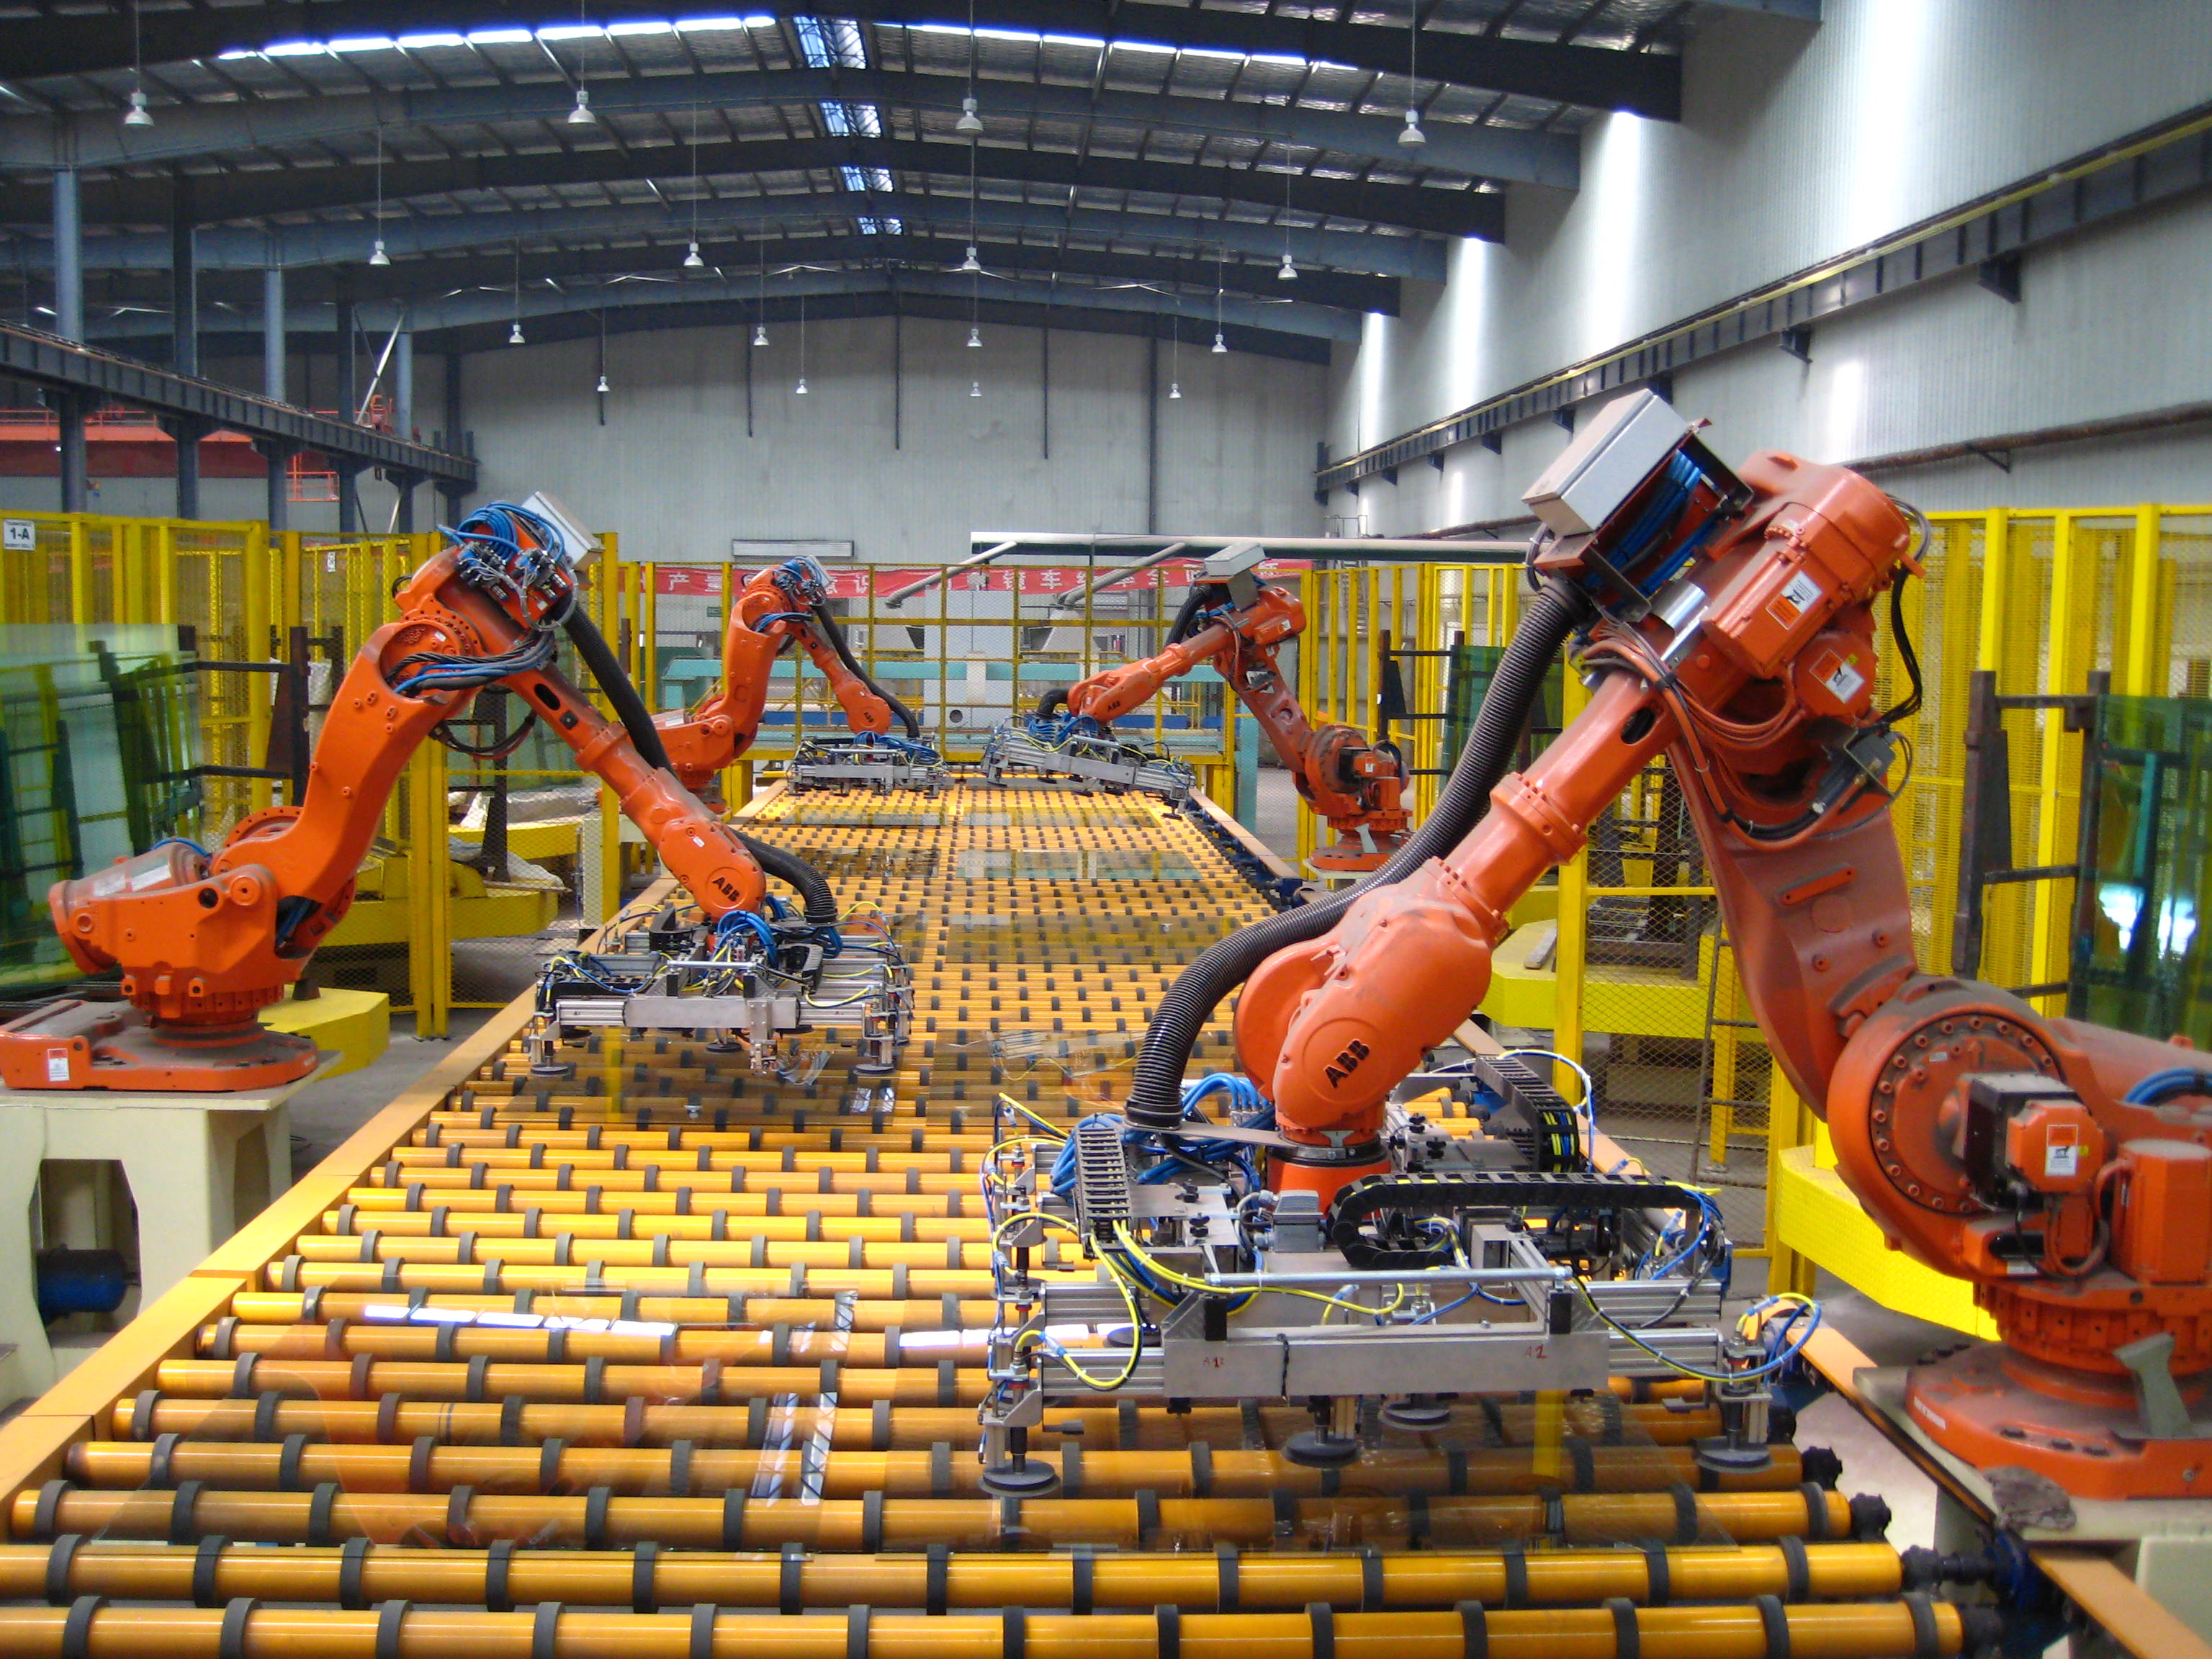
\includegraphics[width=8cm]{figs/industrial_robot.jpg}
    \end{center}
    \caption{Robots en lineas de ensamblaje}
    \label{fig:robIndustrialChain}
  \end{figure}\   

  \item \textit{Soldadura.} Es utilizada en soldadura de estructuras mecánicas debido a su alta precisión y capacidad de realizar 
                            la misma soldadura perfecta una y otra vez. Además, también son usados para soldar placas de circuitos.
  \begin{figure} [h!]
    \begin{center}
      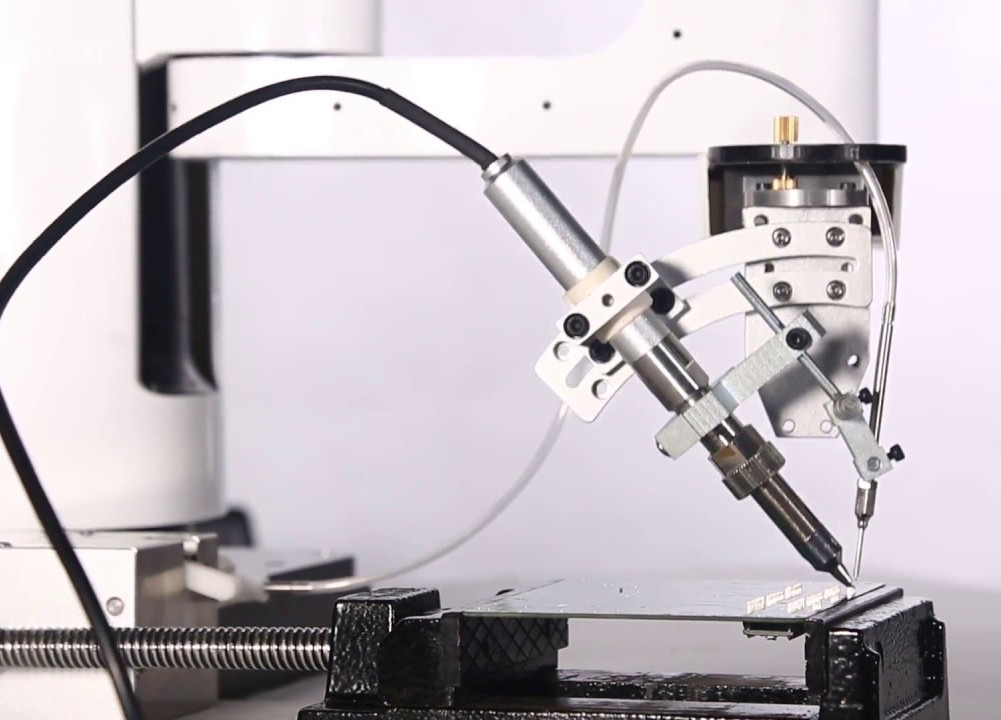
\includegraphics[width=8cm]{figs/solder_robot.jpg}
    \end{center}
    \caption{Robot Dobot M1 realizando una soldadura con estaño}
    \label{fig:robSoldering}
  \end{figure}\ 

  \item \textit{Investigación y desarrollo en laboratorios.} Los brazos robóticos realizan tareas de laboratorio repetitivas y precisas, 
                              lo que puede acelerar el proceso de investigación y desarrollo de nuevos productos médicos. Uno de los usos más 
                              frecuentes es preparar y procesar muestras en investigaciones científicas. En concreto, pueden desempeñar tareas
                              como la extracción de ADN, la separación de componentes, la adición de reactivos y el análisis de muestras 
                              químicas, entre otros. Esto ayuda a reducir los errores humanos y garantizar la integridad y reproducibilidad 
                              de los experimentos llevados a cabo.
  
  \begin{figure} [h!]
    \begin{center}
      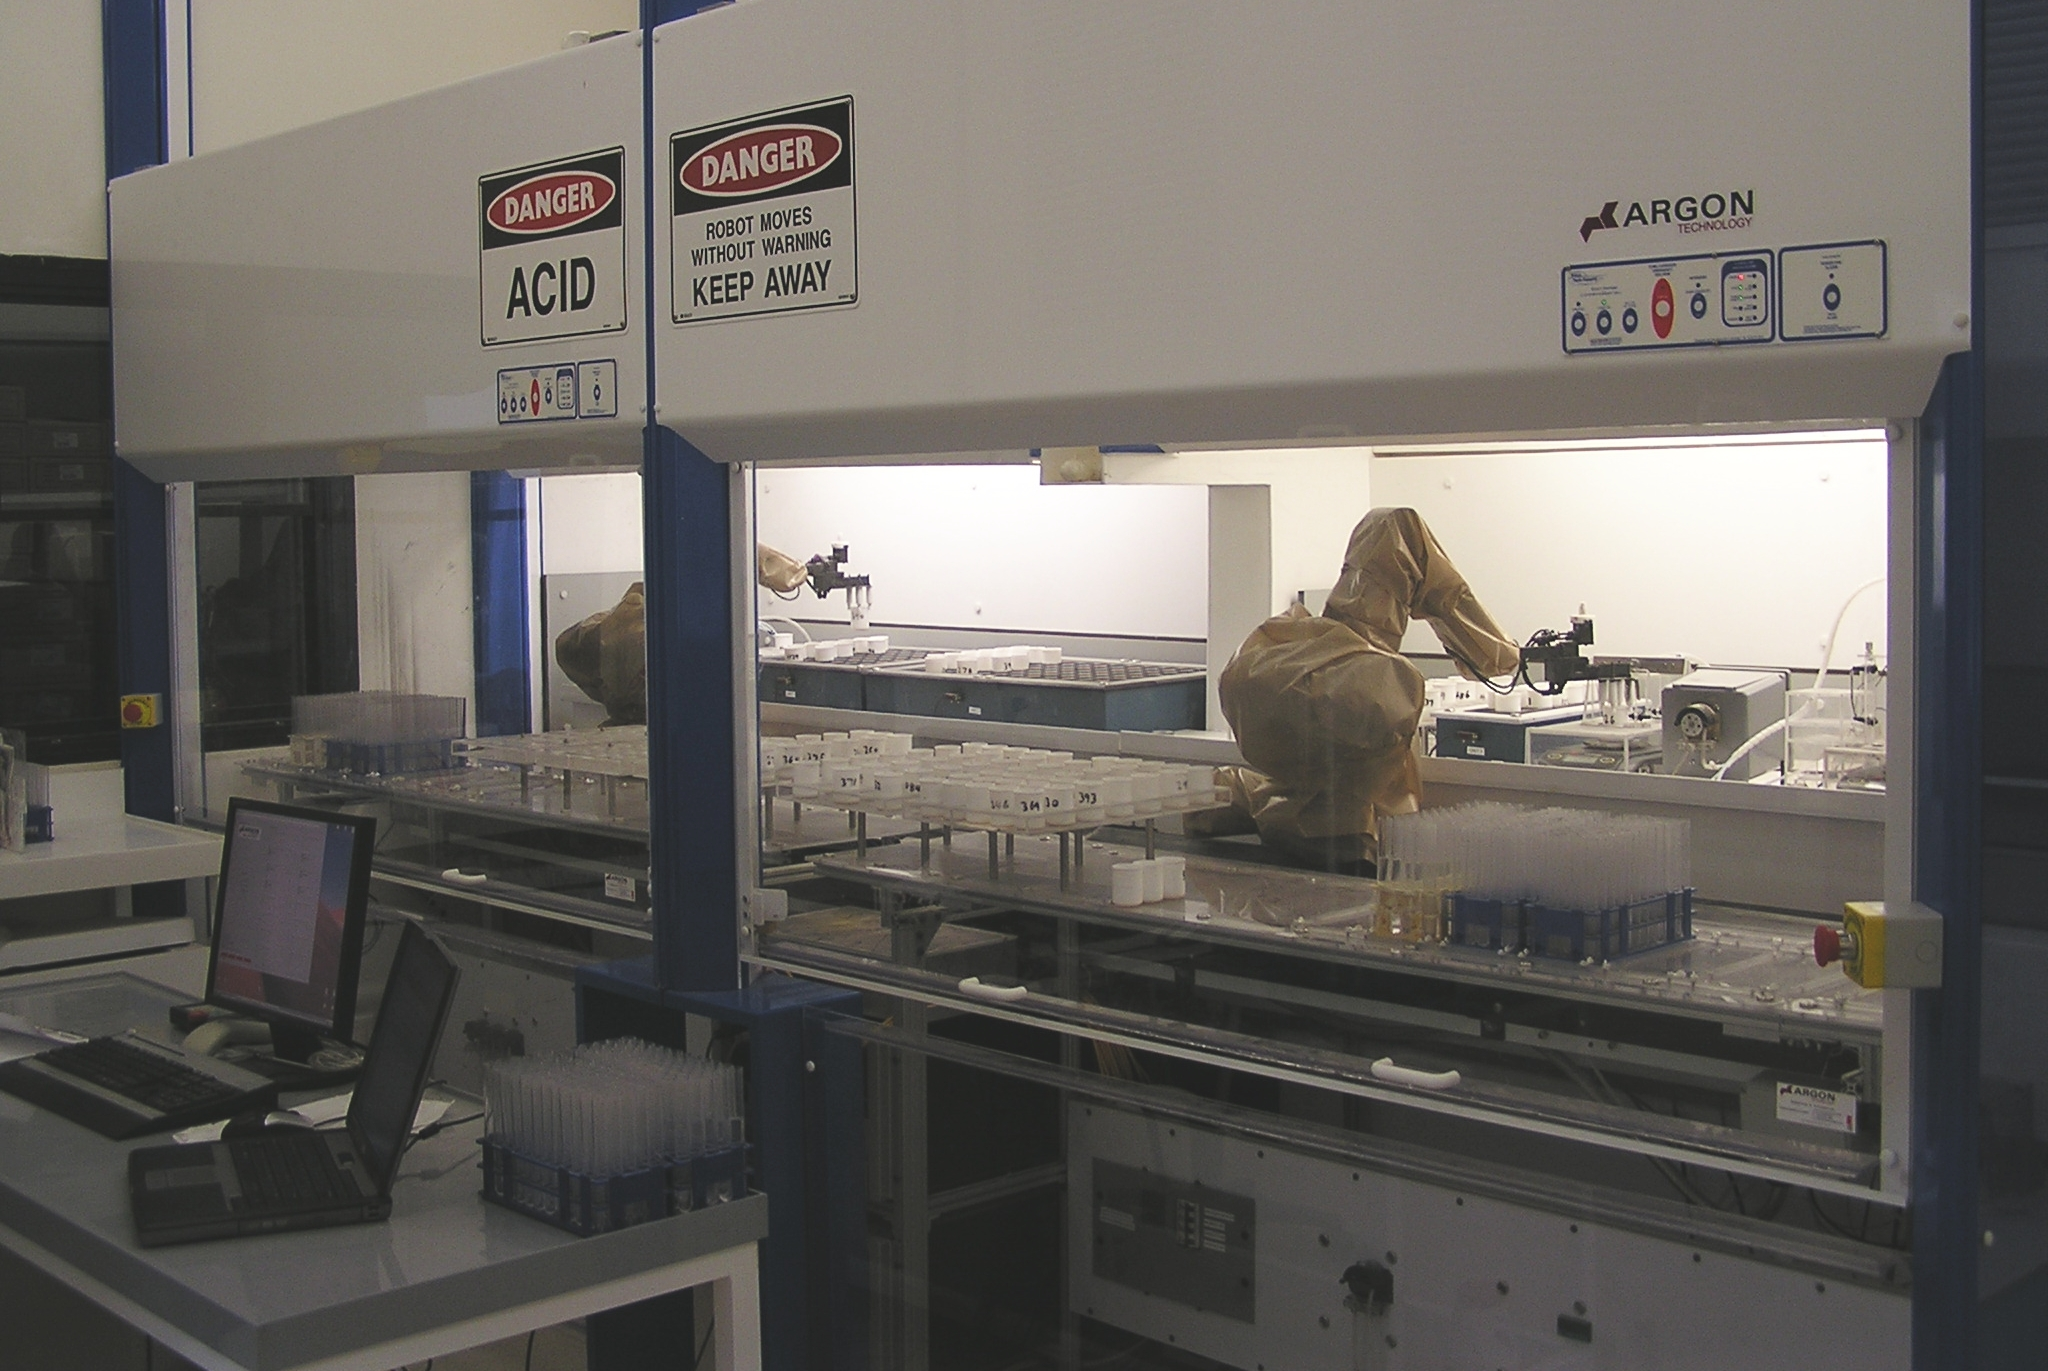
\includegraphics[width=8cm]{figs/lab_robot.jpg}
    \end{center}
    \caption{Robots en el ámbito científico}
    \label{fig:robLaboratory}
  \end{figure}\ 

 \end{itemize}\



\section{Robótica en educación}
\label{sec:segundaseccion}
La robótica en la educación es una disciplina que ha cobrado una gran relevancia en los últimos años debido a la creciente necesidad 
de formar a las nuevas generaciones en competencias tecnológicas. 
\\En las escuelas de secundaria, se ha convertido en una herramienta pedagógica eficaz para desarrollar habilidades y conocimientos en áreas como la programación, 
la matemática, la electrónica y la resolución de problemas. Esto es conocido como \textit{STEM} (Science, Technology, Engineering and Mathematics). Los 
estudiantes aprenden a diseñar, construir y programar robots simples para llevar a cabo una tarea específica, lo que les ayuda a comprender  
los conceptos de ciencia y tecnología de una manera más práctica e interactiva.\\
\begin{figure} [h!]
  \begin{center}
    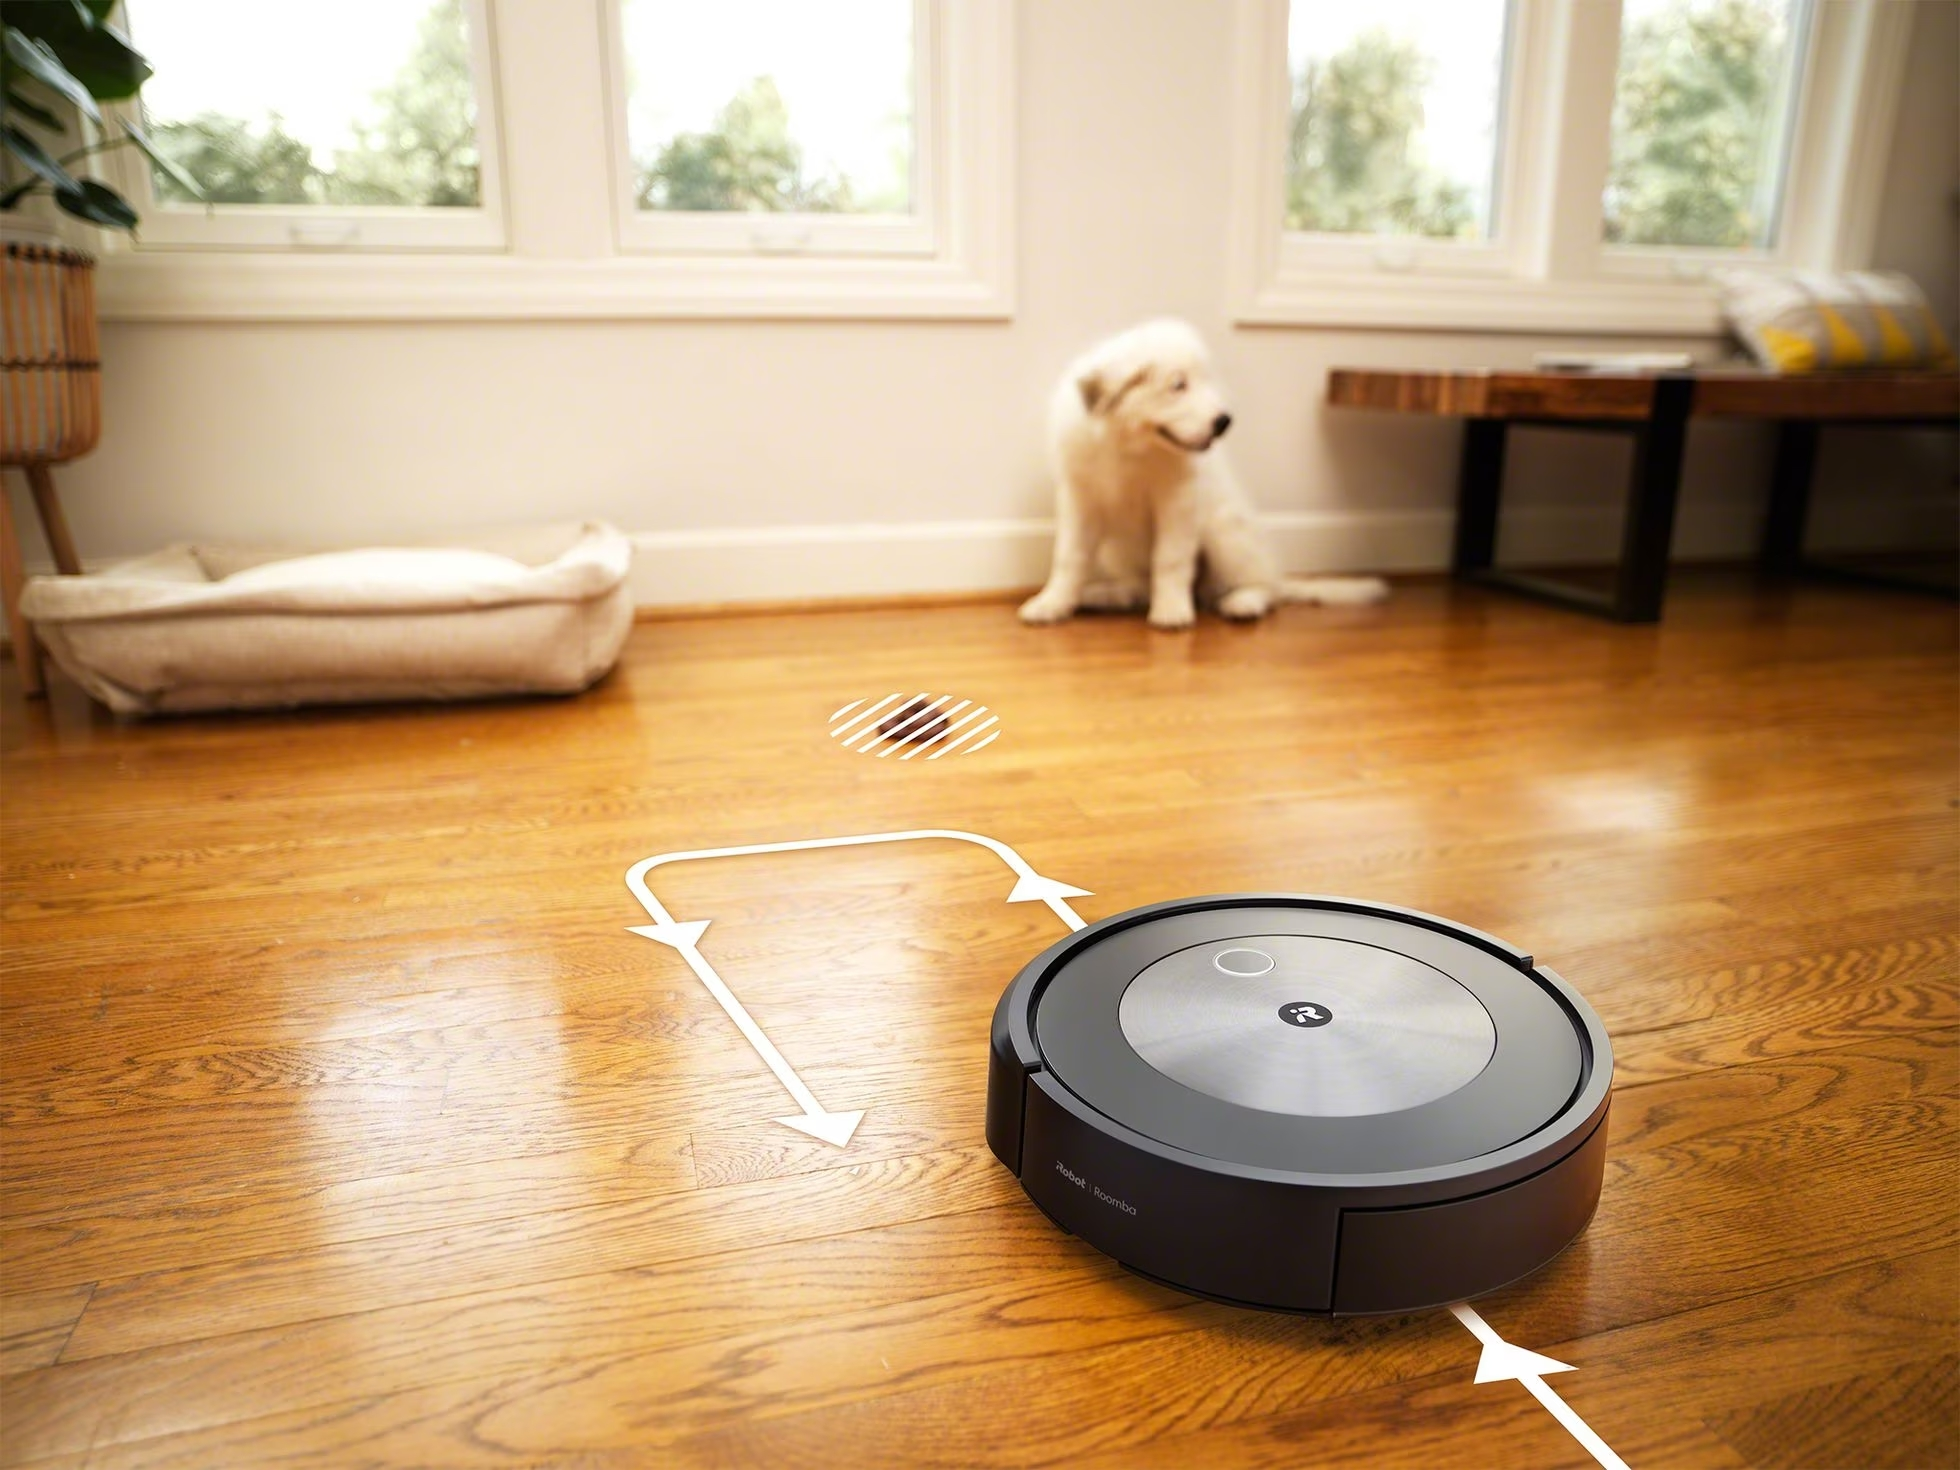
\includegraphics[width=8cm]{figs/roomba}
  \end{center}
  \caption{Robots educativos en la escuela secundaria.}
  \label{fig:robSecundaria}
\end{figure}\
\\En el nivel universitario, la robótica se ha convertido en una disciplina esencial para formar a los futuros ingenieros. Los estudiantes aprenden 
a diseñar y construir robots más avanzados, y refuerzan sus habilidades de programación y control de sistemas complejos. Además se hacen uso de más tipos 
de robot, como pueden ser, industriales o plataformas robóticas móviles reales. Al ser sistemas usados en el mundo profesional, los estudiantes pueden 
aprender con el robot que usará en un futuro. Aunque es verdad que las universidades disponen de algunas unidades, no siempre son accesibles para el 
estudiante por diversas razones.
\newpage

\\En resumen, la robótica en la educación es una herramienta poderosa para fomentar el aprendizaje y la innovación en las nuevas 
generaciones. Desde la escuela hasta la universidad, la robótica se ha convertido en una disciplina clave para formar a los futuros 
líderes tecnológicos del mundo.

No olvides incluir imágenes y referenciarlas, como la Figura \ref{fig:robUniversidades}.

\section{Robótica de bajo coste}
\label{sec:segundaseccion}
La robótica de bajo coste es un área de la robótica enfocada en el diseño y desarrollo de robots 
accesibles y asequibles. El objetivo principal de la robótica de bajo coste es conseguir desarrollar tecnología robótica
barata, reduciendo la complejidad de los sistemas empleados y haciendo uso de materiales más económicos.

La disponibilidad de herramientas de fabricación de bajo costo, como la impresión 3D y el corte láser, 
han hecho posible que los usuarios puedan crear piezas y componentes robóticos personalizados a un 
precio más bajo que el de la fabricación tradicional.

La Ley de Moore es una ley teórica que establece que la capacidad de procesamiento de los microchips se duplica 
cada dos años. Esta observación, pese haberse dado hace casi 60 años, sigue siendo válida a día de hoy. Entre 
otras cosas, es lo que ha permitido el desarrollo de componentes electrónicos cada vez más pequeños, eficientes 
y potentes. La robótica de bajo coste es un claro ejemplo de cómo el crecimiento de la capacidad de computación y 
la disminución de los costes de producción ha llevado al abaratamiento de la robótica y de la electrónica en general.

Gracias a esto, la robótica de bajo coste, se basa en la filosofía `Hazlo tú mismo` o \textit{Do It by Yourself (DIY)} , que se enfoca en la creación de proyectos personalizados y 
asequibles utilizando tecnología de bajo costo y materiales comunes.

En resumen, la robótica de bajo costo es una consecuencia directa del crecimiento de la capacidad de computación, 
el abaratamiento de los precios de los componentes electrónicos y del enfoque \textit{DIY}. Estoque ha permitido la creación 
de robots avanzados y accesibles para el público general.
El desarollo de esta tecnología, permite que más personas puedan experimentar en este área de la ingeniería y desarrollar 
sus propias soluciones robóticas. 
 
\ref{sec:miseccion}

Para hablar de números, mételos en el entorno \textit{math} de \LaTeX, por ejemplo, $1.5Kg$. También puedes usar el símbolo del Euro como aquí: 1.500\euro.

\subsection{Listas}

Cuando describas una colección, usa \texttt{itemize} para ítems o \texttt{enumerate} para enumerados. Por ejemplo:

\begin{itemize}
 \item \textit{Entorno de simulación.} Hemos usado dos entornos de simulación: uno en 3D y otro en 2D.
 \item \textit{Entornos reales.} Dentro del campus, hemos realizado experimentos en Biblioteca y en el edificio de Gestión.
\end{itemize}\


\paragraph{Referencias bibliográficas}
\label{sec:referencias}

Cita, sobre todo en este capítulo, referencias bibliográficas que respalden tu argumento. Para citarlas basta con poner la instrucción \verb|\cite| con el identificador de la cita. Por ejemplo: libros como \cite{vega12e}, artículos como \cite{vega19b}, URLs como \cite{vega19a}, tesis como \cite{vega18b}, congresos como \cite{vega18a}, u otros trabajos fin de grado como \cite{vega08b}.

Las referencias, con todo su contenido, están recogidas en el fichero \texttt{bibliografia.bib}. El contenido de estas referencias está en formato \texttt{BibTex}. Este formato se puede obtener en muchas ocasiones directamente, desde plataformas como \texttt{Google Scholar} u otros repositorios de recursos científicos.

Existen numerosos estilos para reflejar una referencia bibliográfica. El estilo establecido por defecto en este documento es APA, que es uno de los estilos más comunes, pero lo puedes modificar en el archivo \texttt{memoria.tex}; concretamente, cambiando el campo \verb|apalike| a otro en la instrucción \verb|\bibliographystyle{apalike}|. 

\

\

\

Y, para terminar este capítulo, resume brevemente qué vas a contar en los siguientes.


\chapter{Estado del arte}
\label{cap:capitulo2}
\noindent En este capítulo se describen algunos de los trabajos más relevantes publicados sobre robots industriales en educación.

En \cite{KRIMPENIS2020103} se presenta una solución industrial barata para crear un robot capaz de hacer operaciones de mecanizado (fabricación 
de piezas mediante operaciones de corte). Este robot se llama HydraX y esta dotado de 6 grados de libertad. Tiene un alcance máximo de casi un metro, un 
peso que ronda los 13 Kg y está fabricado mediante impresión 3D. 
Además, tiempo después, se publicó la segunda parte de este artículo \cite{PAPAPASCHOS2020109}, en el cual se aborda el diseño software y de control 
que se ha desarrollado para controlar dicho brazo. \\
    \begin{figure} [h!]
        \begin{center}
          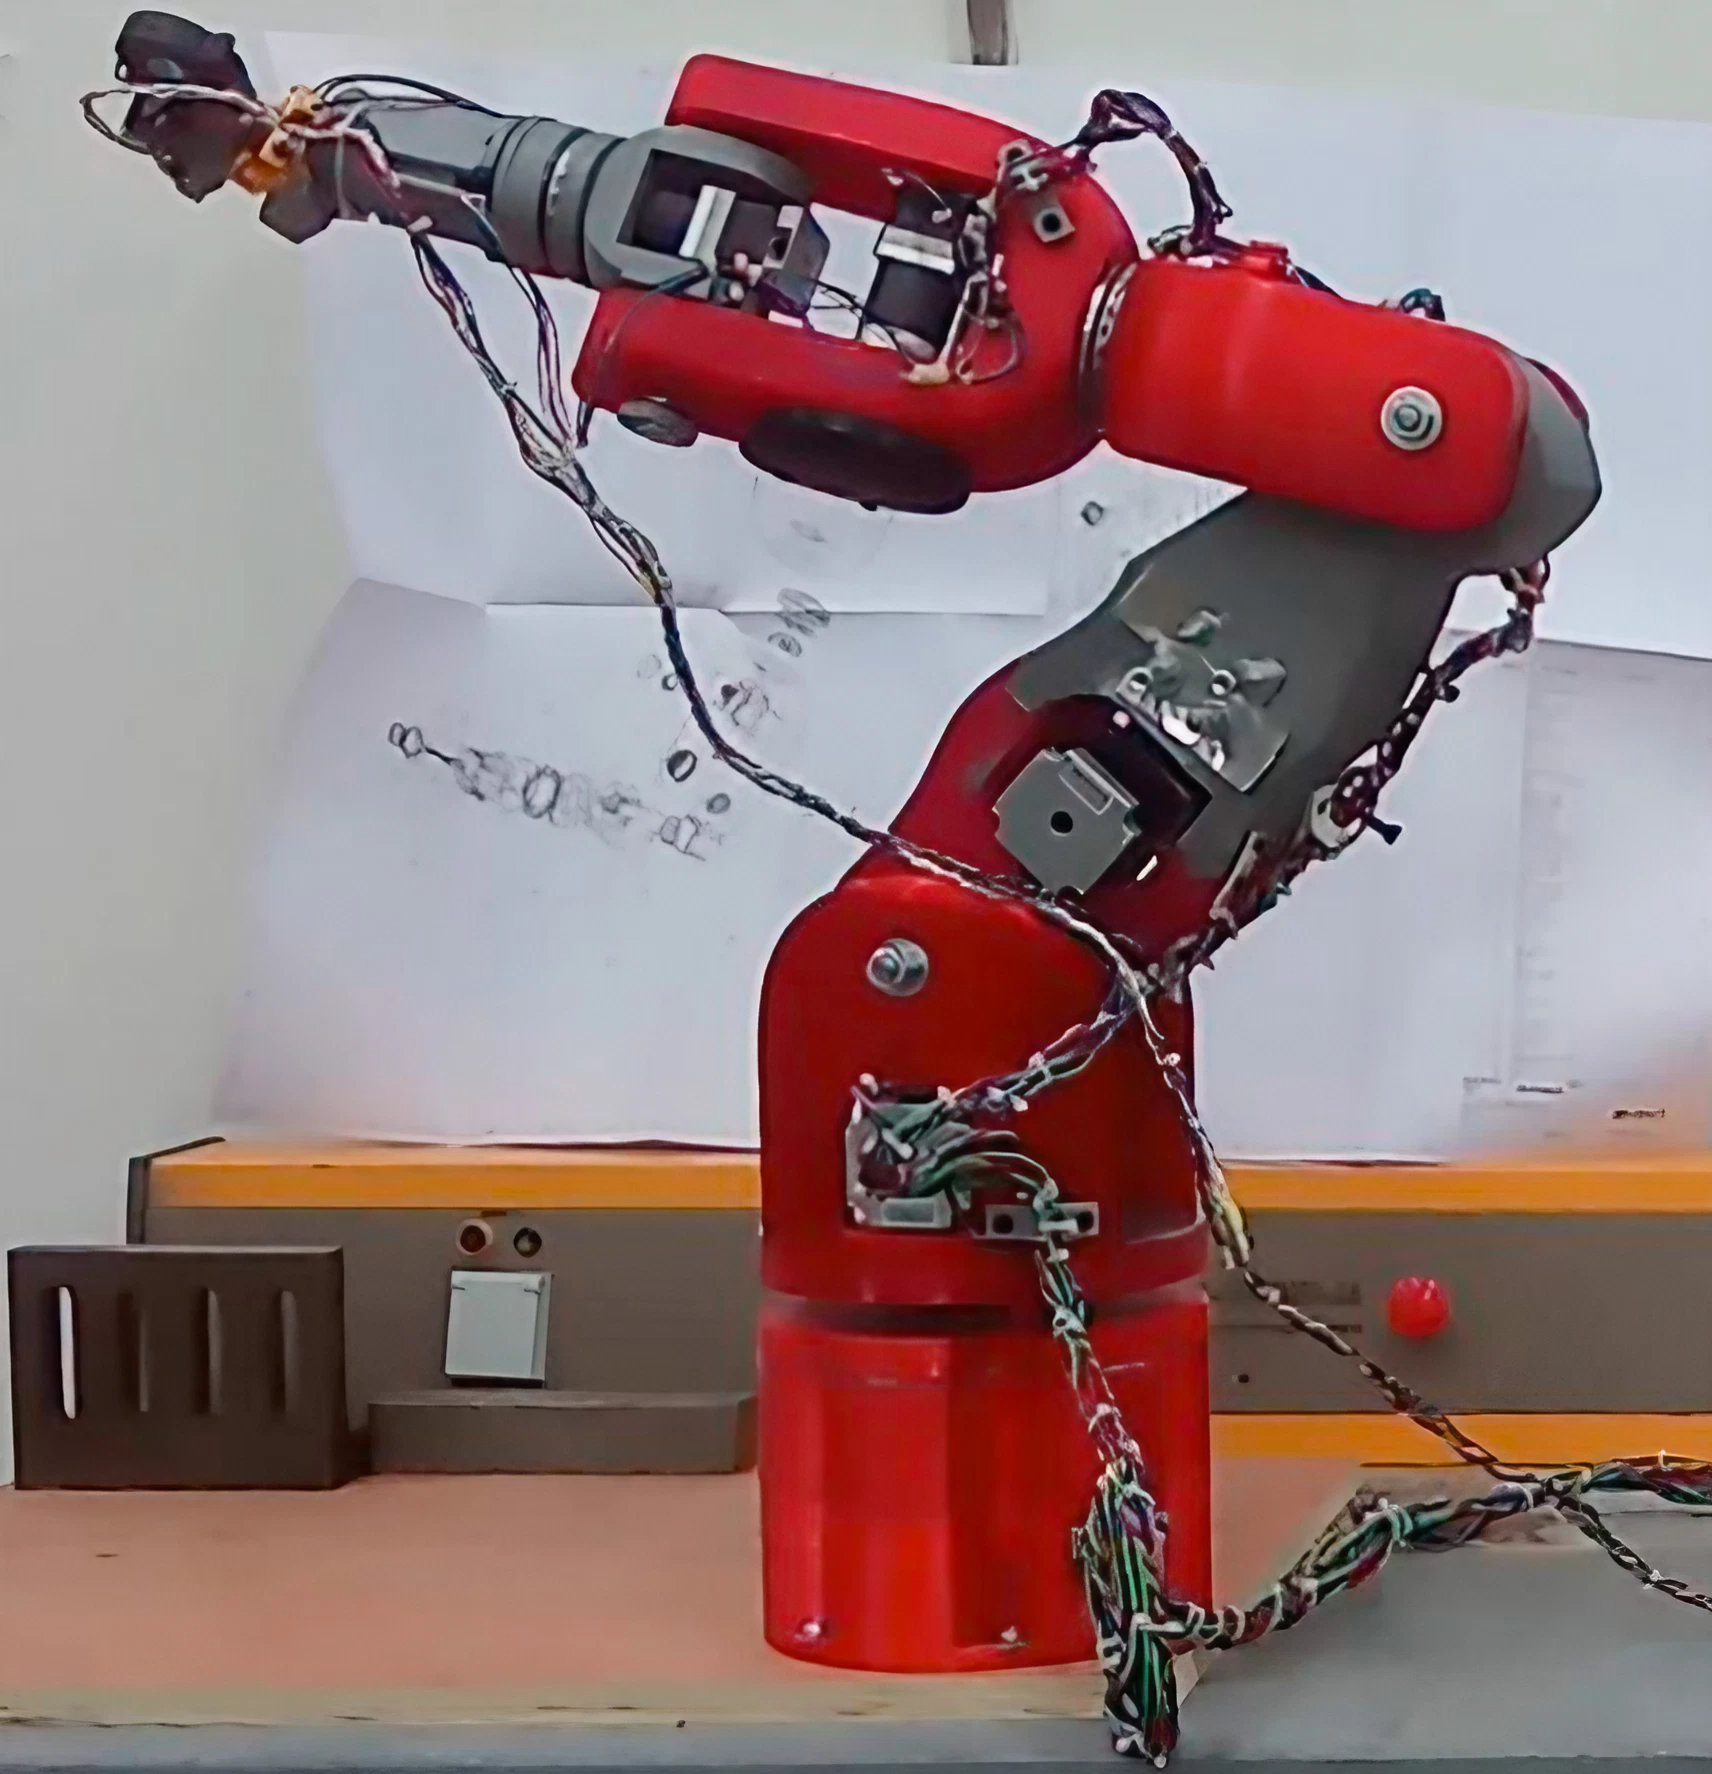
\includegraphics[width=6cm]{figs/Hydra.png}
        \end{center}
        \caption{Robot HydraX}
        \label{fig:hydra}
    \end{figure}\ 
    \newpage
    Los puntos fuertes del proyecto son los siguientes:
    \begin{itemize}
        \item Tiene una repetitividad de ±0.04 mm.
        \item Tiene un espacio de trabajo muy amplio.
        \item Tener más de 3 grados de libertad le permiten alcanzar gran cantidad de puntos con distintas orientaciones.
        \item Según el artículo, tiene una capacidad de carga máxima de 12 kilogramos. A pesar de esto, se comenta que en la práctica el peso en el 
        extremo del robot debe ser menor a 5 Kg, por lo que su carga útil rondará los 3 Kg para un funcionamiento aceptable. Esto lo sitúa a la par 
        del robot comercial ABB IRB 120\footnote{\url{https://new.abb.com/products/es/3HAC031431-001/irb-120}}  
    \end{itemize}\
    
    Y estos son los puntos débiles que cabe mencionar:
    \begin{itemize}
        \item Carece de integración en \ac{ROS}, plataforma de desarrollo de la que se habla en la Sección \ref{subsec:ros2}.
        \item Su coste en materiales supera los 1000 \euro \xspace , por lo que no es lo suficientemente asequible para su uso académico.
        \item Según este artículo, se necesitan 200 horas para poder imprimir y montar el brazo, lo que implica que es costoso en tiempo 
        crear varias unidades, además de que requiere de cierta habilidad para construirlo correctamente.
        \item En este artículo no se proporcionan los ficheros necesarios para poder crearlo. Además, se menciona que las piezas han sido 
        diseñadas mediante el software privativo SolidWorks\textsuperscript{\tiny\textregistered}, por lo que lo hace más difícil y costoso de editar.
    \end{itemize}\
    \newpage
    Existen soluciones más sencillas y reproducibles, como por ejemplo, la presentada en \cite{adediran2023uiarm}. En este trabajo se describe 
    un brazo robótico 
    cuyo propósito es separar botellas de plástico en un proceso de reciclaje. Más allá de la aplicación que se le pretende dar, 
    lo mas importante es que se hace uso de  
    un manipulador de tamaño reducido, impreso en 3D y con 4 \ac{DOF}.
    \begin{figure} [ht!]
        \begin{center}
          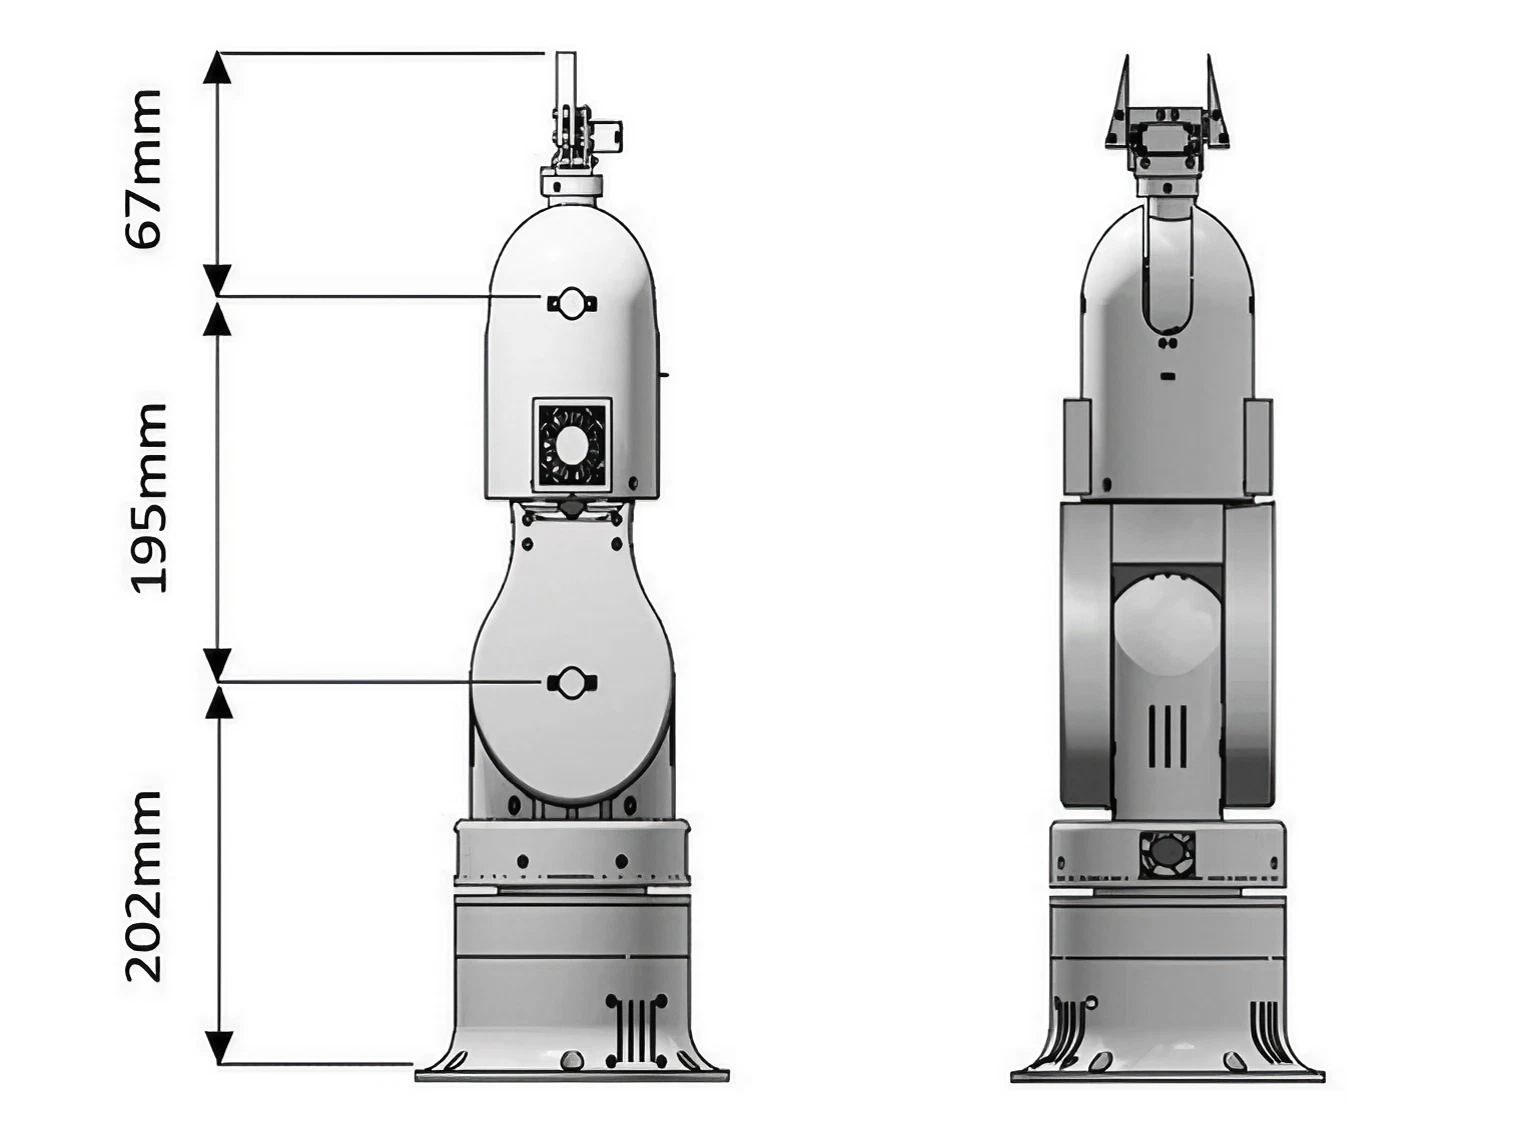
\includegraphics[width=8cm]{figs/uiarm.png}
        \end{center}
        \caption{Robot UIArm}
        \label{fig:uiarm}
    \end{figure}\ 
    
    A partir de la información proporcionada en este artículo, se han extraído los siguientes puntos fuertes:
    \begin{itemize}
        \item El diseño de las piezas se ha realizado mediante el uso de la herramienta de diseño \nameref{subsec:freecad}, esto supone una ventaja respecto 
        a \cite{KRIMPENIS2020103}, que utilizaba una herramienta privativa.
        \item Utiliza motores de pequeño tamaño con una reductora integrada, lo que aumenta su torque y abarata en gran medida los costes 
        del robot. Debido a esto, el consumo de energía es menor pudiendo hacer uso de una electrónica compacta y menos costosa.
        \item Al estar compuesto por menos piezas y tener pocos grados de libertad, se requiere menos tiempo para imprimir y construir este robot.
    \end{itemize}\
    Y estos son puntos negativos que cabría destacar:
    \begin{itemize}
        \item El espacio de trabajo (puntos del espacio alcanzables por el extremo del brazo) del robot es demasiado reducido. Esto es debido 
        a la disposición de los grados de libertad. Utiliza dos de ellos para cambiar la orientación del extremo del robot, dejando solo dos para el 
        posicionamiento, por lo que es imposible en la práctica abarcar todo el espacio 3D al alcance del brazo.
        \item Utiliza engranajes impresos en 3D para rotar la segunda articulación comenzando desde la base. Debido a esto, pierde exactitud en función 
        de la posición del brazo debido a la holgura de este tipo de transmisión.
        \item Carece de integración con \ac{ROS} y el autor no proporciona otro tipo de software que permita desarrollar programas para este robot perjudicando la 
        continuidad del proyecto.
    \end{itemize}\

    Otro desarrollo \textit{low-cost} que ha adquirido gran popularidad
    gracias a la plataforma KickStarter \footnote{\url{https://www.kickstarter.com/projects/niryo/niryo-one-an-open-source-6-axis-robotic-arm-just-f/description}} 
    es el robot Niryo One, que es un brazo robot impreso en 3D con 6 grados de libertad, en la cual fue 
    capaz de recaudar 80.000\euro \xspace de los 20.000 \euro \xspace necesarios. 


    Este proyecto busca dar una alternativa de bajo coste al robot convencional usado por \textit{makers}, estudiantes y 
    pequeñas compañías. Para lograrlo, apuesta por el uso de componentes comunes y la filosofía \textit{Open Source}, la cual se basa en la 
    idea de compartir, colaborar y democratizar el acceso al conocimiento y al software. Por ello, su código fuente y planos están disponibles 
    de forma gratuita para que cualquier persona interesada pueda acceder a ellos.

    Aunque este modelo no es el más nuevo de la marca Niryo, sí es el que más comunidad tiene y más extendido está.
    Este robot y los modelos posteriores, pueden ser adquiridos a través de su página oficial \footnote{\url{https://niryo.com/products-cobots/niryo-one/}}.
    \\
    \begin{figure} [ht!]
        \begin{center}
          
\includegraphics[width=11cm]{figs/niryo.png}
        \end{center}
        \caption{Robot Niryo One}
        \label{fig:niryo}
    \end{figure}\ 
    \newpage
    Este proyecto destaca positivamente por:
    \begin{itemize}
    \item El proyecto completo es de código abierto y se puede encontrar toda la electrónica necesaria y documentos para imprimirlo en 
    su repositorio de github \footnote{\url{https://github.com/NiryoRobotics/niryo_one}}.
    \item Tiene integración con ROS 1 y MoveIt.
    \item Cuenta con 6-DOF, lo que permite alcanzar gran cantidad de puntos con distintas orientaciones.
    \item Cuenta con una repetitividad de 0.5mm y puede levantar hasta 300g.
    \item Permite adaptar una gran variedad de herramientas diferentes.
    \item Es capaz de detectar colisiones gracias a sus motores codificados mediante sensores magnéticos.
    \end{itemize}
    En cambio, tiene los siguientes inconvenientes:
    \begin{itemize}
    \item Hace uso de una placa Raspberry Pi en vez de una placa Arduino/Esp32, lo que incrementa el coste del equipo. 
    \item Hablando del precio, el coste de este equipo comprado en su versión en aluminio ronda los 3500\euro. El coste de fabricación 
    de este robot mediante el uso de impresión 3D ronda los 1000\euro \xspace según este artículo \footnote{\url{https://www.zdnet.com/article/this-mini-industrial-robot-is-less-than-1k/}}
    \item Aunque proporcionan los ficheros fuentes del diseño, este ha sido realizado mediante SolidWorks\textsuperscript{\tiny\textregistered} por 
    lo que no puede ser editado sin tener que pagar por el programa.
    \item Pese a tener integración con ROS1, el proyecto no ha sido adaptado de forma oficial para ROS2, por lo que es necesario 
    usar un sistema operativo antiguo (Ubuntu 16.04) del año 2016. O bien utilizar Ros Bridge \footnote{\url{https://github.com/ros2/ros1\_bridge}} 
    para comunicar el ROS 1 de la placa con un  ordenador moderno con ROS 2.
    \end{itemize}
    \newpage
    En el ámbito de los robots caseros, se puede destacar un referente reconocido, MeArm. Se trata de un 
    brazo mecánico de diseño simple y completamente \textit{OpenSource}. De hecho, tal es su repercusión, que miles de personas 
    se han impreso el suyo o creado su propia versión mejorada. Prueba de ello es la cantidad de modificaciones que se han ido subiendo a  
    páginas como Thingiverse\footnote{\url{https://www.thingiverse.com/search?q=mearm&page=1&type=things&sort=relevant}}. Además, existen 
    robots con diferentes nombres basados en el mismo concepto, como puede ser EEZYBotArm, una versión más robusta y atractiva que el original. \\
    Consta de 3 grados de libertad y de una pinza simple. Todos los motores del robots son servomotores de 9 gramos y se basa en el uso de 
    paralelogramos para transferir el movimiento de los motores al extremo del robot, manteniendo el peso de los mismos en la base. 

    \begin{figure} [h!]
        \centering    
        \subfigure[MeArm]{\label{fig:mearm}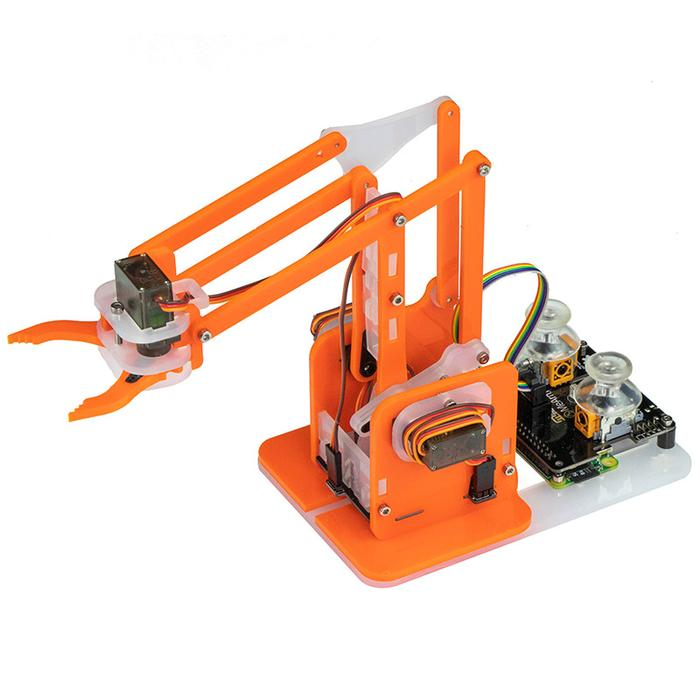
\includegraphics[width=0.3\linewidth ]{figs/mearm.jpg}}
        \hspace{3cm}
        \subfigure[EEZYBotArm MK1]{\label{fig:eezy}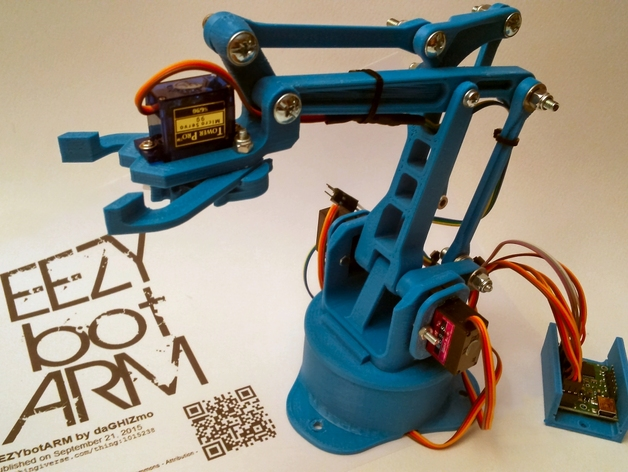
\includegraphics[width=0.3\linewidth]{figs/eezy.jpg}}
        \caption{Robots formados a partir de paralelogramos}
    \end{figure}
    
    Se trata de un proyecto muy extendido, con una comunidad que ha creado muchas variantes de él, por lo que para evaluar los puntos fuertes y 
    débiles del robot, se va a hacer referencia al robot original MeArm V1.
    Los aspectos significativos de este robot son:
    \begin{itemize}
        \item Se trata de un proyecto totalmente accesible y replicable, ya que usa pocos materiales y estos son fáciles de adquirir.
        \item El centro de masa del robot se concentra en la base, reduciendo la inercia del brazo y permitiendo así movimientos más rápidos.
        \item No requiere de apenas tiempo de impresión y el montaje es sencillo gracias a las numerosas guías de 
        montaje\footnote{\url{https://docs.rs-online.com/2bb1/0900766b81593e58.pdf}} que circulan por internet.
        \item Al usar servomotores, se puede establecer el ángulo de cada articulación fácilmente sin necesitar de ningún tipo de sensor externo.
        \item Debido a su forma y materiales utilizados, tiene un peso muy reducido pudiéndose acoplar a robots móviles sin afectar a 
        su rendimiento.
    \end{itemize}
    En cuanto a sus limitaciones, se deben mencionar:
    \begin{itemize}
    \item Se suele prescindir del uso de rodamientos en sus articulaciones. Esto reduce el tiempo de vida del brazo debido a que el propio rozamiento 
    de los ejes acaba desgastando el plástico, creando holguras que afectan directamente en la precisión. Esta holgura obliga a apretar en exceso los tornillos 
    que hacen de ejes de las articulaciones, aumentando el rozamiento y reduciendo fuerza útil de los pequeños motores.
    \item Este robot está limitado en cuanto a fuerza debido al uso de servomotores. Usa los típicos SG90 o similares con un torque de apenas 
    0.16 Newton-metro. El uso de servos más grandes aumenta significativamente el precio del dispositivo. 
    \item Los servomotores padecen de vibraciones al conectarle una carga. Esto hace que el conjunto tiemble en exceso durante los movimientos.
    \end{itemize}

\noindent Una vez se han presentado los proyectos más relevantes en este campo, se procederán a definir una serie 
de requisitos y objetivos concretos para dar solución al problema que se plantea en este trabajo.


\chapter{Objetivos}
\label{cap:capitulo3}

\begin{flushright}
\begin{minipage}[]{10cm}
\emph{Un objetivo sin un plan es solo un deseo}\\
\end{minipage}\\

Antoine de Saint-Exupéry\\
\end{flushright}

\vspace{1cm}

Tras haber enmarcado el contexto en el cual se encuentra este trabajo de fin de grado, se procede a realizar
una descripción del problema, requisitos, metodología y plan de trabajo usado.
\section{Descripción del problema}
\label{sec:descripcion}
Este trabajo de fin de grado nace de la necesidad de abordar el problema existente en nuestra universidad, donde la escasez de 
robots disponibles y la dificultad para acceder a ellos han limitado nuestra experiencia práctica en robótica. 
Estos dispositivos son costosos, lo que limita su disponibilidad, y su fragilidad impide que los estudiantes 
interactúen plenamente con ellos por temor a dañarlos. Además, la cantidad limitada de robots en relación con el número de carreras que 
quieren utilizarlos, crea una gran competencia por su uso. Sumado a ello, los profesores tienen que hacer frente a la burocracia asociada al 
uso de los mismos. 
La solución propuesta busca superar estas limitaciones al proporcionar a la enseñanza un robot casero impreso en 3D, que será
económico, accesible y útil en el aprendizaje práctico de los estudiantes. 
Por lo tanto, el objetivo principal de este trabajo de fin de grado es desarrollar un brazo robótico que pueda ser empleado en la 
asignatura de Robótica Industrial de esta universidad. Asimismo, se busca que el sistema creado sea asequible y fácilmente replicable haciendo uso de las impresoras 3D de la universidad.\\
Con el fin de alcanzar esta meta, se ha dividido el proyecto en los siguientes subobjetivos:

\begin{enumerate}
    \item Realizar una investigación acerca de los robots que actualmente están disponibles y que cumplan con 
          las características y objetivos deseados. Estos robots deberán tener un tamaño y costo similar, y 
          preferiblemente haber sido impresos en 3D. Se dará mayor relevancia a aquellos que utilicen un software y hardware 
          libres.
    \item Explorar diversas opciones de diseño para determinar la forma ideal del robot. Se analizará cuidadosamente 
          qué tipo de robot se ajusta mejor al uso que se le pretende dar, así como los grados de libertad necesarios. 
            
    \item Realizar una investigación exhaustiva sobre los componentes de hardware disponibles en el mercado, con el fin de seleccionar 
          aquellos que mejor se adapten a las necesidades y objetivos de construir un robot eficiente y funcional. Se llevará 
          a cabo un análisis detallado de los precios y características de cada componente, para seleccionar aquellos 
          que ofrezcan la mejor relación calidad-precio. Una vez evaluados todos los aspectos, se elegirá un conjunto 
          final de componentes para construir el robot de manera efectiva. 
    
    \item Realizar el \ac{CAD} del brazo. Se pretende hacer uso de FreeCad\footnote{\url{https://www.freecad.org/index.php?lang=es_ES}}, entre otras herramientas, para
          diseñar en 3D cada pieza que constituirá el robot. Puesto a que debe ser imprimible en una impresora \acs{FDM} convencional,
          debe estar pensado para no necesitar soportes y utilizar el mínimo material posible.
    \item Emplear una impresora 3D convencional para materializar los diseños realizados anteriormente.
    \item Programar el software necesario para poder controlar el robot desde el ordenador.
    \item Realizar la integración del robot realizado en el ecosistema \ac{ROS}. 

  
\end{enumerate}\


\section{Requisitos}
\label{sec:requisitos}
Con el fin de solucionar el problema descrito, se han establecido los siguientes requisitos:
\begin{enumerate}
      \item Se espera un brazo robot de tipo industrial de bajo coste cuya fabricación completa esté por debajo de 200\euro.
      \item La mayoría de las partes que componen el robot, deben ser imprimibles en cualquier impresora 3D convencional.
      \item A fin de poder garantizar la portabilidad del robot, este debe de tener un consumo inferior a 25 vatios.
      \item En cuanto a sus dimensiones, se busca un tamaño idóneo para su uso sobre un escritorio. Esto implica que no necesariamente 
      tiene que estar unido al suelo, permitiendo su fácil traslado.
      \item Es necesario que sea simple de montar y esté compuesto del menor número de piezas posibles con el fin de poder crear varias unidades 
      en poco tiempo. 
      \item Se busca continuidad en el proyecto a largo plazo, por lo que debe tener integración con el ecosistema \acs{ROS} 2. 

\end{enumerate}\

\section{Metodología}
\label{sec:metodologia}

Durante el desarrollo del trabajo se ha establecido un protocolo de reuniones semanales con el tutor a 
través de la plataforma Teams, con el objetivo de compartir los avances realizados y recibir retroalimentación 
sobre el trabajo. Además, cada semana se han propuesto las actividades a realizar, asegurando así una adecuada 
planificación y coordinación del proyecto. \\
Para el desarrollo del sistema se ha utilizado un repositorio en la plataforma GitHub\footnote{\url{https://github.com/RoboticsURJC/tfg-vperez}}, en el cual se ha ido
subiendo el código y diseños generados a lo largo del proyecto. Adicionalmente, en este mismo repositorio 
se ha incluido una Wiki\footnote{\url{https://github.com/RoboticsURJC/tfg-vperez/wiki}} con las explicaciones detalladas de todas las actividades llevadas a cabo durante estos 
meses de trabajo. De esta manera, se ha creado un registro completo y accesible de todo el proceso de desarrollo del sistema.

\section{Plan de trabajo}
\label{sec:plantrabajo}
El desarrollo del TFG ha estado dividido en dos etapas. La primera, comenzó en octubre y fue abandonada en enero. 
//TODO

\chapter{Plataforma de desarrollo}
\label{cap:capitulo4}

\begin{flushright}
\begin{minipage}[]{10cm}
\emph{Las herramientas adecuadas en las manos adecuadas pueden cambiar el mundo}\\
\end{minipage}\\
Steve Jobs\\
\end{flushright}

\vspace{1cm}
Tras haber establecido los objetivos que se pretenden alcanzar en este trabajo de fin de grado, se procede a describir
las herramientas \textit{software} y \textit{hardware} utilizadas para lograrlos. 

\section{Software}
\label{sec:software}
Llamamos \textit{software} al conjunto de programas, instrucciones y datos que dotan de lógica al sistema.
\subsection{Python}
\label{subsec:pyhton}
Python es un lenguaje de programación, es decir, una serie de reglas gramaticales bien definidas que le proporciona a una persona, en este 
caso el programador, la capacidad de programar una serie de instrucciones o secuencias de órdenes con el fin de crear un comportamiento 
lógico determinado. 

Se trata de un lenguaje de alto nivel interpretado. Cuando se dice que un lenguaje es de alto nivel, se hace referencia a su nivel de 
abstracción y facilidad de uso en comparación con los lenguajes de bajo nivel, es decir, aquellos que te permiten mayor control sobre los 
componentes físicos del sistema. Decimos que es un lenguaje interpretado debido a que no es necesario convertir el texto escrito por el humano en 
instrucciones entendibles por un procesador previamente a su ejecución. Esto agiliza el proceso de desarrollo ya que la conversión de código humano a 
código máquina (compilación) suele demorar un tiempo. Por el contrario, la ejecución de un programa en lenguaje compilado es más rápida.  

Una de las características más destacadas de Python es su amplia librería (conjunto de código destinado a un objetivo concreto) estándar, que proporciona 
variedad de módulos y funciones para realizar multitud de tareas. Como cualquier otro lenguaje de programación, cuenta con una gran cantidad de librerías de terceros que 
amplían sus capacidades, como SciPy en la ciencia de datos, Django en el desarrollo web, Numpy para operar con matrices, TensorFlow el aprendizaje automático, entre otros.

\subsection{Grbl}
\label{subsec:grbl}
Grbl\footnote{\url{https://github.com/gnea/grbl}} es un firmware de código abierto usado para controlar máquinas llamadas \acs{CNC}. Este firmware se ejecuta en 
un microcontrolador, que se encuentra dentro de la controladora de la máquina \acs{CNC}, en nuestro caso, la placa base del robot. \\
Básicamente, convierte las instrucciones de código G, que posteriormente hablaremos de él, en señales eléctricas que se envían a los motores de la máquina. Además, 
comprueba los diferentes sensores de la máquina, como pueden ser los finales de carrera, para establecer los límites físicos de cada movimiento. \\
Grbl es flexible por lo que podemos cambiar la configuración para adaptarla a un caso de uso concreto. De hecho, aunque solo soporta movimientos lineales,
en este trabajo se abordará la configuración necesaria para para poder usar las articulaciones rotativas del nuestro robot.
\begin{figure} [h!]
  \begin{center}
    
\includegraphics[width=4cm]{figs/grbl.png}
  \end{center}
  \caption{Logo de Grbl}
  \label{fig:grbllogo}
\end{figure}\ 
\subsection{Código G}
\label{sec:gcode}
\textit{G-code}, también conocido como RS-274, es el nombre del lenguaje de programación más usado en máquinas de \ac{CNC}. 
Proporciona control numérico basado en métricas para equipos controlados por \ac{CAM}, como pueden ser, fresadoras y tornos. 
La programación de este lenguaje precisa de una sintaxis específica en la que se emplean letras y números para representar 
diferentes comandos y parámetros. Por ejemplo, la letra "G" seguida de un número indica un comando de movimiento, mientras 
que la letra "M" seguida de un número se utiliza para comandos misceláneos, como el encendido o apagado del láser/motor de fresado.
Así es como se programan los movimientos necesarios para que la herramienta realice una trayectoria cuadrada en el plano XY:
\begin{verbatim}
  G90       ; Establecer modo de posicionamiento absoluto
  G21       ; Establecer unidad de medida en milímetros
  F200      ; Establecer velocidad de avance a 200 unidades por minuto 
  
  G0 X0 Y0  ; Mover a la posición inicial (esquina inferior izquierda) 
  G1 X20    ; Mover horizontalmente hacia la derecha 20 mm
  G1 Y20    ; Mover verticalmente hacia arriba 20 mm
  G1 X0     ; Mover horizontalmente hacia la izquierda 20 mm
  G1 Y0     ; Mover verticalmente hacia abajo 20 mm
  G0 X0 Y0  ; Volver a la posición inicial (esquina inferior izquierda)
  
  M2        ; Fin del programa
\end{verbatim}

\subsection{FreeCAD}
\label{subsec:freecad}
FreeCAD\footnote{\url{https://www.freecad.org/index.php?lang=es_ES}} es una aplicación de diseño asistido por ordenador de código abierto y gratuita, utilizada para el modelado de piezas en 3D .
Está dirigida al mundo de la ingeniería mecánica y el diseño de productos, pero también es usada en arquitectura y otros campos.
\\FreeCAD utiliza modelado paramétrico. Se trata de un enfoque de diseño que utiliza parámetros y relaciones entre ellos para 
crear modelos 3D modificables, lo que permite realizar un cambio en la geometría modificando el valor de un cierto parámetro.
También ofrece una variedad de bancos de trabajo (\textit{work benches}) especializados, como \textit{Part Design}, \textit{Sketcher} y \textit{Draft} para adaptarse a diferentes 
necesidades de diseño. Además, permite incluir nuevas herramientas y funcionalidades creadas por la comunidad, mediante su administrador 
de complementos.
\\FreeCAD cuenta con una comunidad activa de usuarios que contribuyen al desarrollo y la mejora continua del software. Gracias a esto, 
es sencillo aprender a utilizarlo a partir de las numerosas guías de uso y tutoriales.
\begin{figure} [h!]
  \begin{center}
    
\includegraphics[width=4cm]{figs/freecad.png}
  \end{center}
  \caption{Logo de FreeCAD}
  \label{fig:freecadlogo}
\end{figure}\ 

\subsection{ROS 2}
\label{subsec:ros2}
ROS, por sus siglas en inglés, significa \textit{Robot Operating System}. Se trata de una plataforma de código abierto utilizada 
para desarrollar y controlar sistemas robóticos.
El objetivo principal de ROS es facilitar el desarrollo de sistemas robóticos al proporcionar una infraestructura que permite que
los desarrolladores pueden centrarse en la lógica y el comportamiento específico de los robots, sin tener que preocuparse por la 
infraestructura de comunicación y control. 
Además, proporciona una colección de bibliotecas, herramientas y convenios que permiten a los programadores crear software para robots. 
También proporciona herramientas para la visualización de datos, simulación de robots, depuración y pruebas. Además, 
cuenta con una comunidad activa de usuarios y desarrolladores que contribuyen con paquetes adicionales y comparten su 
conocimiento.

Está diseñado para ser modular, lo que permite la creación de sistemas complejos mediante la reutilización de otros componentes existentes.

Una de las características distintivas de ROS es su arquitectura basada en nodos. Los nodos son procesos independientes 
que se comunican entre sí mediante mensajes. Cada nodo puede realizar tareas específicas, en función de la lógica atribuída por el programador.

En este trabajo se utiliza ROS 2, la versión sucesora de ROS. Esta versión incorpora gran variedad de mejoras respecto a su anterior versión. En esta versión 
los nodos no dependen de un nodo \textit{Master} para comunicarse ya que las comunicaciones están distribuidas mediante el uso de \ac{DDS}. Esto 
incrementa la robusted del sistema y reduce significativamente los tiempos de latencia. \\
La distribución de utilizada en este trabajo es \textit{ROS 2 Humble}. Se trata de la última versión de ROS estable disponible para Ubuntu 22.04 LTS.
\begin{figure} [h!]
  \begin{center}
    
\includegraphics[width=4cm]{figs/ros2logo.jpeg}
  \end{center}
  \caption{Logotipo de ROS 2 Humble}
  \label{fig:ros2logo}
\end{figure}\ 

\subsection{MoveIt!}
\label{subsec:moveit}
MoveIt es una plataforma de desarrollo (\textit{framework}) para manipulación robótica de código abierto que permite desarrollar 
aplicaciones de manipulación complejas utilizando ROS. Además, proporciona una amplia gama de herramientas y bibliotecas que 
facilitan el control y planificación de movimientos de robots. Con MoveIt, puedes crear fácilmente aplicaciones que permitan
a los robots realizar tareas de manipulación avanzadas, como agarrar objetos, ensamblar piezas y mover el brazo en entornos complejos. 
Es altamente flexible gracias a su diseño modular y se puede utilizar con una gran variedad de robots. De hecho, incorpora la herramienta 
\textit{MoveIt Setup Assistant}; se trata de una asistente de configuración con interfaz gráfica que te permite generar los ficheros 
necesarios para utilizar tu propio robot en este ecosistema. 
\begin{figure} [h!]
  \begin{center}
    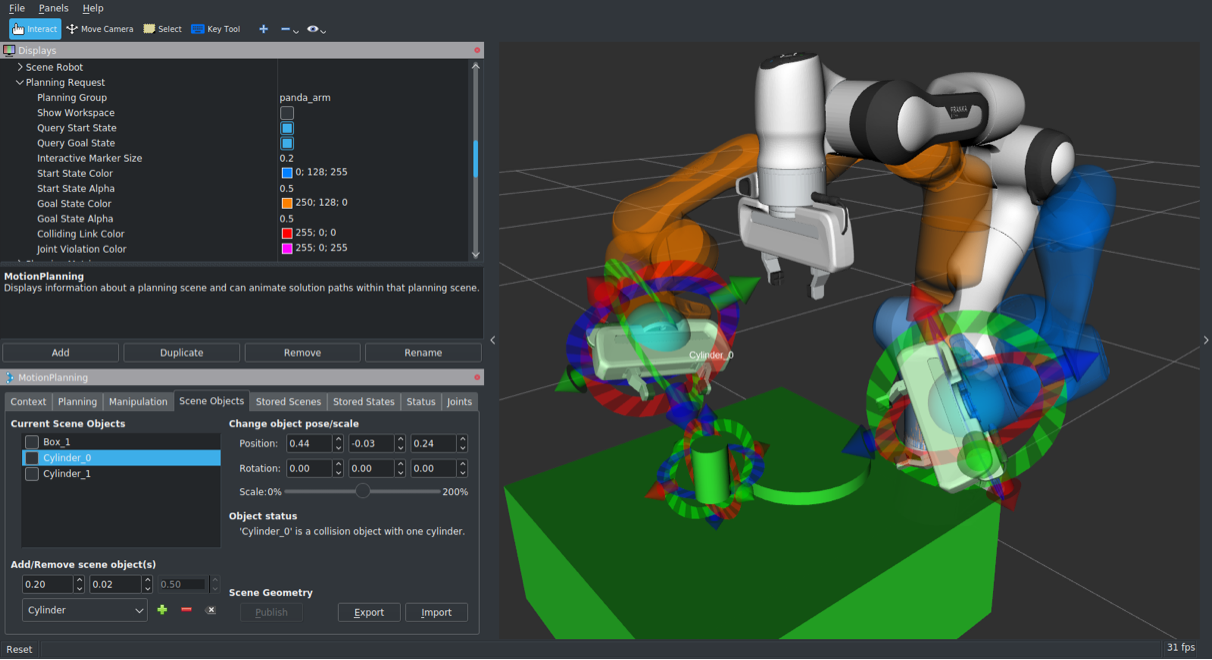
\includegraphics[width=12cm]{figs/moveit_intro.png}
  \end{center}
  \caption{Aspecto del plugin de MoveIt para Rviz2 (Franka Emika Robot)}
  \label{fig:ros2logo}
\end{figure}\ 

\section{Hardware}
\label{sec:hardware}
Cuando hablamos de \textit{hardware}, nos referimos a todos los componentes físicos de utilizados en el dispositivo electrónico, en este caso, un robot. Estos 
componentes son tangibles, es decir, se pueden tocar y ver.

\section{MKS DLC32}
\label{subsec:mksdlc32}
Se trata de una placa destinada al mundo de las máquinas de grabado láser. Ha sido creada por \textit{MakerBase} y es considerada 
\textit{Open Hardware} por lo que toda la información de la placa puede encontrarse en su repositorio de Github\footnote{\url{https://github.com/makerbase-mks/MKS-DLC32}}.
Es fácilmente adquirible por \textit{Aliexpress} por un precio que ronda los 16\euro. Está basada en el microcontrolador de 32 bits: ESP32. 
Se trata de un dispositivo muy asentado en la comunidad \textit{maker} debido a su bajo coste e integración en el 
ecosistema Arduino. De hecho, gracias a su conectividad wifi y bluetooth ha ganado terreno a los microcontroladores Atmega que incorporan los propios Arduinos.\\
Esta placa es ideal para este proyecto debido a que cuenta con la posibilidad de controlar 
hasta 3 motores y es completamente compatible con \nameref{subsec:grbl}. Además dispone de una salida de potencia regulable controlable mediante \nameref{subsec:grbl} que nos 
permite alimentar dispositivos. Estos podrían ser: electroimán (tipo de imán que es activado mediante electricidad), motor \ac{CC} entre otros. Además se puede aprovechar las salidas \ac{PWM} para conectar un grabador láser o un servo. 
El rango de funcionamiento es de 12 a 24 voltios por lo que es adecuado para ser alimentado mediante baterías y con cargadores de ordenador. 
\begin{figure} [h!]
    \begin{center}
      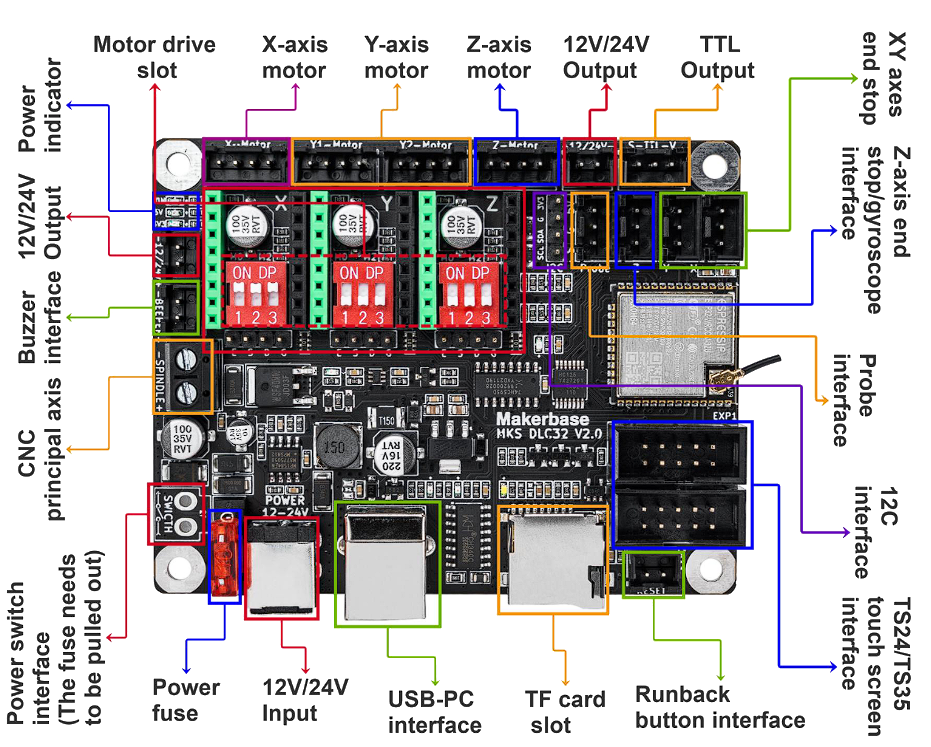
\includegraphics[width=10cm]{figs/MKS.png}
    \end{center}
    \caption{Placa base MakerBase DLC32}
    \label{fig:robSoldering}
  \end{figure}\ 

\section{Motores Nema 17}
\label{subsec:motores}
Un motor paso a paso es un tipo de motor que se mueve en pequeños pasos o incrementos discretos en lugar de girar continuamente. Estos pasos 
son controlados por señales eléctricas que hacen girar al motor una cantidad específica de grados cada vez que se envía una señal. Debido a que se tiene 
control sobre su avance son una excelente opción si se quiere tener un motor que sea capaz de posicionarse en un ángulo concreto con exactitud. A pesar
de su gran precisión, los motores paso a paso convencionales no tienen el conocimiento absoluto de su posición, por lo que todos los movimientos son 
relativos. Esto hace que se requiera de un \textit{homing} (proceso en el cual la máquina CNC lleva las partes móviles a una 
posición conocida) en el arranque de la máquina para conocer su estado antes de operar.
Para este trabajo, se han usado 3 motores Nema 17 de 60 milímetros de largo debido a las necesidades calculadas más adelante. Son motores bipolares de 
2.1 amperios y una resistencia de 1,6 ohmios con un torque máximo de 0.65 newton-metro.
\begin{figure} [h!]
    \begin{center}
      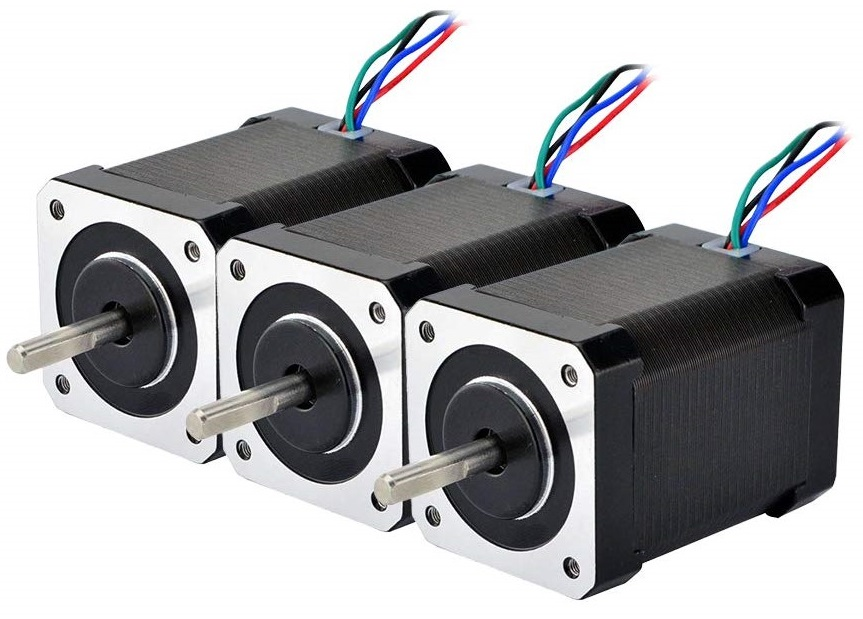
\includegraphics[width=8cm]{figs/nema17.jpg}
    \end{center}
    \caption{Motores Nema 17 de 2.1A}
    \label{fig:robSoldering}
  \end{figure}\ 

\begin{table}[H]
\begin{center}
\begin{tabular}{|c|c|}
\hline
\textbf{Parámetros} & \textbf{Valores} \\
\hline
Nombre del motor & 17HS24-2104S \\
Tipo de motor & Bipolar \\
Ángulo de paso & 1.8º \\
Resistencia de fase & 1.6$\Omega$ \\
Corriente máx. de fase & 2.1A \\
Torque de sujección & 0.65Nm. \\
Dimensiones & 42x42x60mm \\
Peso & 500g \\
Diámetro del eje & 5mm \\
Longitud del eje & 24mm \\
\hline
\end{tabular}
\caption{Especificaciones técnicas de los motores utilizados}
\label{cuadro:ejemplo}
\end{center}
\end{table}

\section{Controlador TMC2209}
\label{subsec:controladorPAP}
Un controlador paso a paso es el módulo hardware capaz de trasformar las señales lógicas que le envía el controlador en una serie de pulsos de
potencia que excitarán las bobinas del motor en un cierto orden para lograr el movimiento. 
Existen motores bipolares, unipolares e híbridos. La diferencia entre ellos radica en la disposición de las bobinas de su interior. Los más usados 
en impresoras 3D y CNC son los bipolares. Son reconocibles debido a que tienen 4 cables.
En este tipo de placas base se pueden instalar distintos modelos de controladores. Cada uno de ellos tiene unas prestaciones diferentes y por tanto 
un precio distinto. Unos ofrecen mayor capacidad de corriente (para controlar motores más grandes), pulsos más suaves que reducen el 
ruido sonoro y las vibraciones, medición en tiempo real de la corriente consumida para conocer el final de una articulación, entre otras tecnologías.  
\begin{figure} [h!]
    \begin{center}
      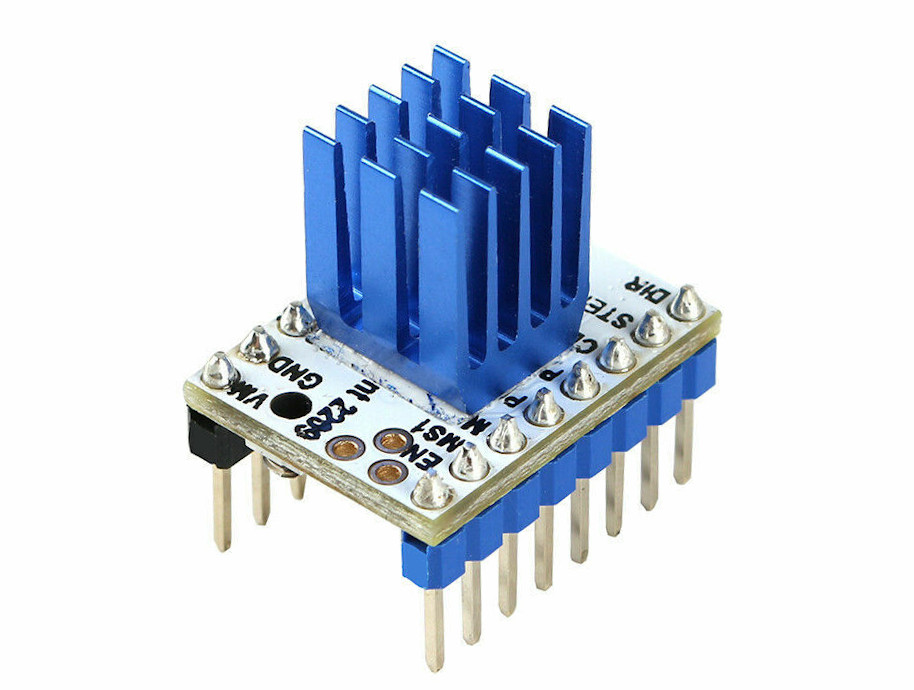
\includegraphics[width=6cm]{figs/TMC2209.jpg}
    \end{center}
    \caption{Controlador TMC2209}
    \label{fig:robSoldering}
\end{figure}\ 

\begin{table}[H]
\begin{center}
\begin{tabular}{|c|c|}
\hline
\textbf{Parámetros} & \textbf{Valores} \\
\hline
Nombre del controlador & TMC2209 \\
Voltaje lógico & 3 - 5V \\
Voltaje de alimentación & 5.5 - 28V \\
Microsteps & Hasta 1/256 \\
Corriente máx. de fase (RMS) & 2A \\
Pérdida de conducción (RDS) & 0.2$\Omega$ \\
Interfaz de comunicación & Pines CFG y UART \\
\hline
\end{tabular}
\caption{Especificaciones técnicas del TMC2209}
\label{cuadro:ejemplo}
\end{center}
\end{table}
    
\newpage
\section{Fuente de alimentación genérica}
\label{subsec:fuente_alimentacion}
Para alimentar el brazo se va a utilizar una fuente de alimentación genérica de 24 voltios y 6 amperios. Este tipo de fuentes pueden ser 
fácilmente adquiribles por internet por un precio aproximado de 15\euro. A pesar de esto, puede ser usada cualquier tipo de fuente capaz de 
entregar más de 20 vatios en el rango de voltaje 12-24v. Más adelante se aborda el uso de cargadores de ordenadores portátiles para alimentar el 
brazo.

\begin{figure} [h!]
  \centering    
  \subfigure[Fuente de alimentación 24v 5A]{\label{fig:pw24}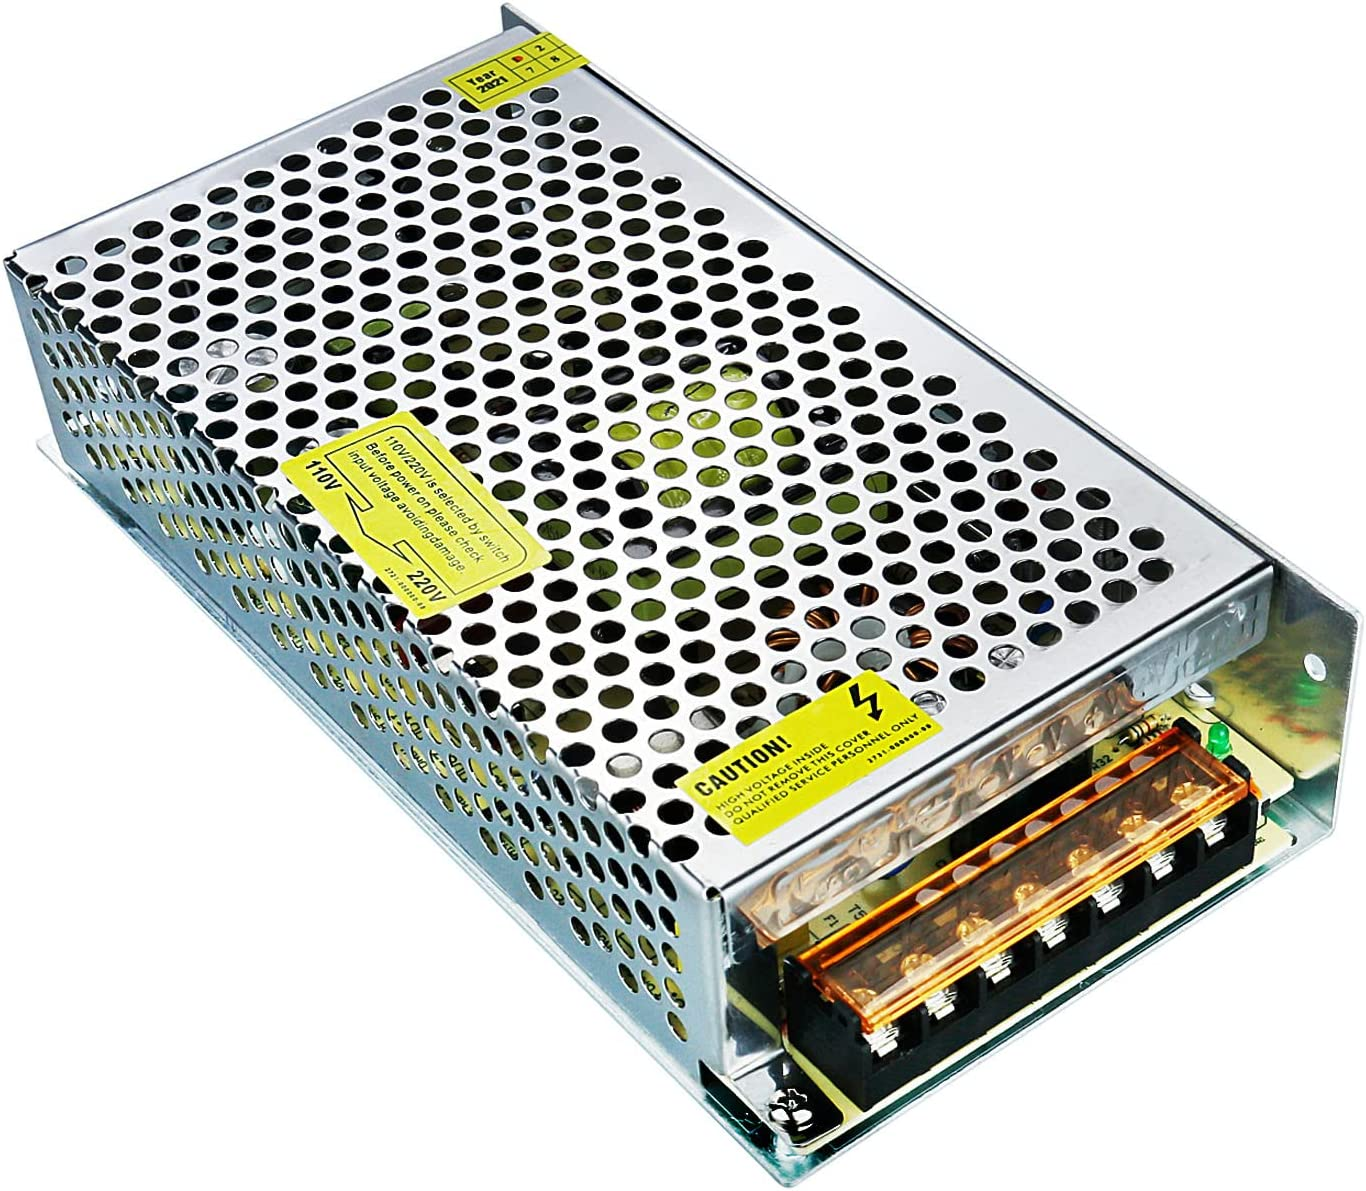
\includegraphics[width=0.55\linewidth ]{figs/pw24v.jpg}}
  \hspace{3cm}
  \subfigure[Cargador de portátil genérico]{\label{fig:pw19}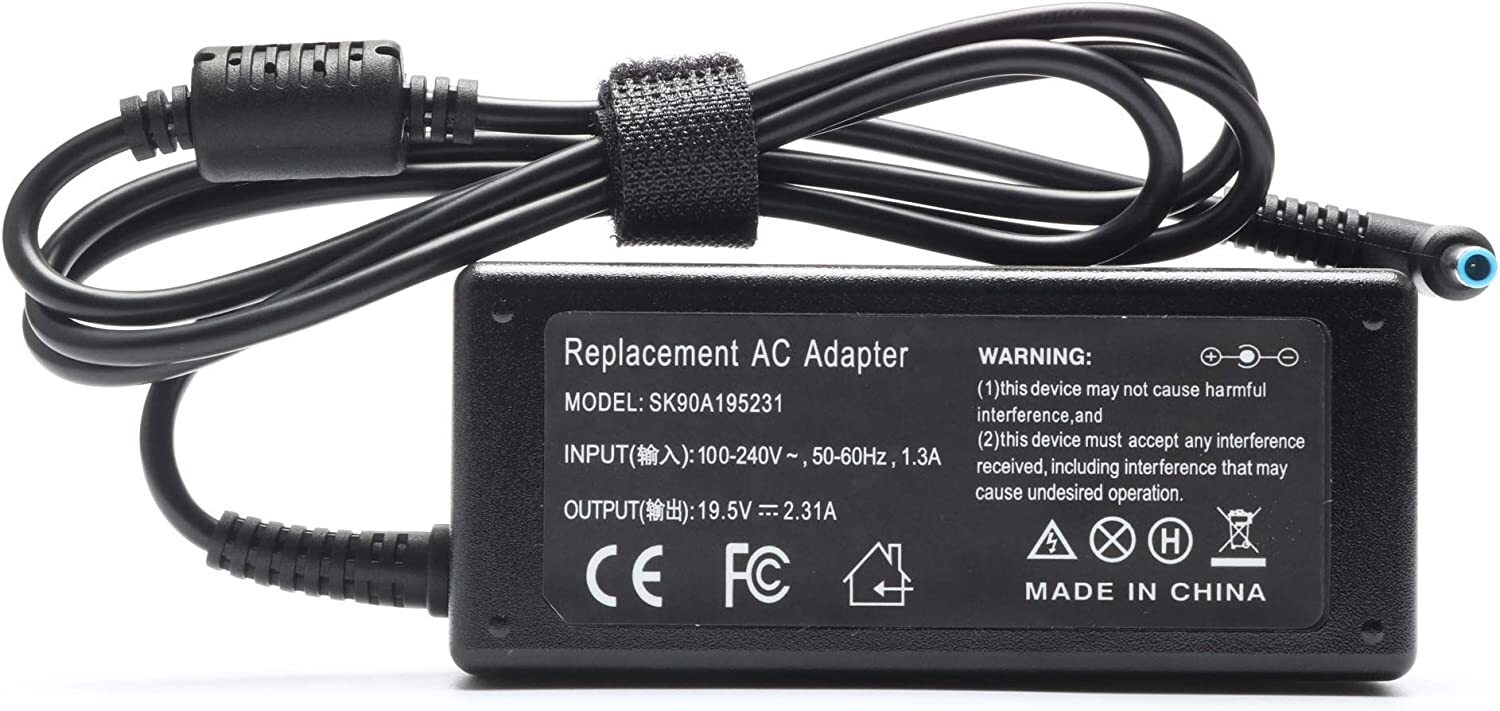
\includegraphics[width=0.55\linewidth]{figs/pw19v.jpg}}
  \caption{Métodos usados para alimentar el robot}
\end{figure}




\chapter{Desarrollo hardware del manipulador}
\label{cap:capitulo5}

\vspace{1cm}

En este capítulo se aborda el desarrollo necesario para, a partir de un concepto, acabar construyendo un prototipo real funcional. Se 
hace incisión en cada etapa necesaria para este cometido.


Escribe aquí un párrafo explicando brevemente lo que vas a contar en este capítulo. En este capítulo (y quizás alguno más) es donde, por fin, describes detalladamente qué has hecho y qué experimentos has llevado a cabo para validar tus desarrollos.

\section{Concepto}
En esta sección se expone como ha sido el proceso de encontrar y definir la idea fundamental del robot, en función de 
los objetivos propuestos, evaluando las distintas opciones para encontrar el que mejor se adapte. Se trata de balance

Primero, se debe conocer el numero de grados de libertad que se ajuste a los requisitos establecidos en la sección \ref{sec:requisitos}. En base 
a los requisitos 1 y 5, que limitan en cuanto a precio de fabricación y complejidad de los mismos, se ha decidido limitar los grados de 
libertad a un máximo de 4. 

hablamos del tipo de joints que existente

Con 4 grados de libertad vamos mal pero se puede.
Tipos:
Scara

RR

Basado en paralelos

\section{Modelo alámbrico}
\subsection{En qué consiste}
\label{subsec:eqc_mod_alambrico}
El modelo alámbrico es una forma de analizar el movimiento de un sistema mecánico compuesto por ejes y eslabones. Este 
enfoque simplifica la representación visual al destacar las relaciones espaciales entre las diferentes partes del sistema mediante 
líneas y conexiones simbólicas, en lugar de mostrar detalles realistas del manipulador. 
\begin{figure} [h!]
  \begin{center}
    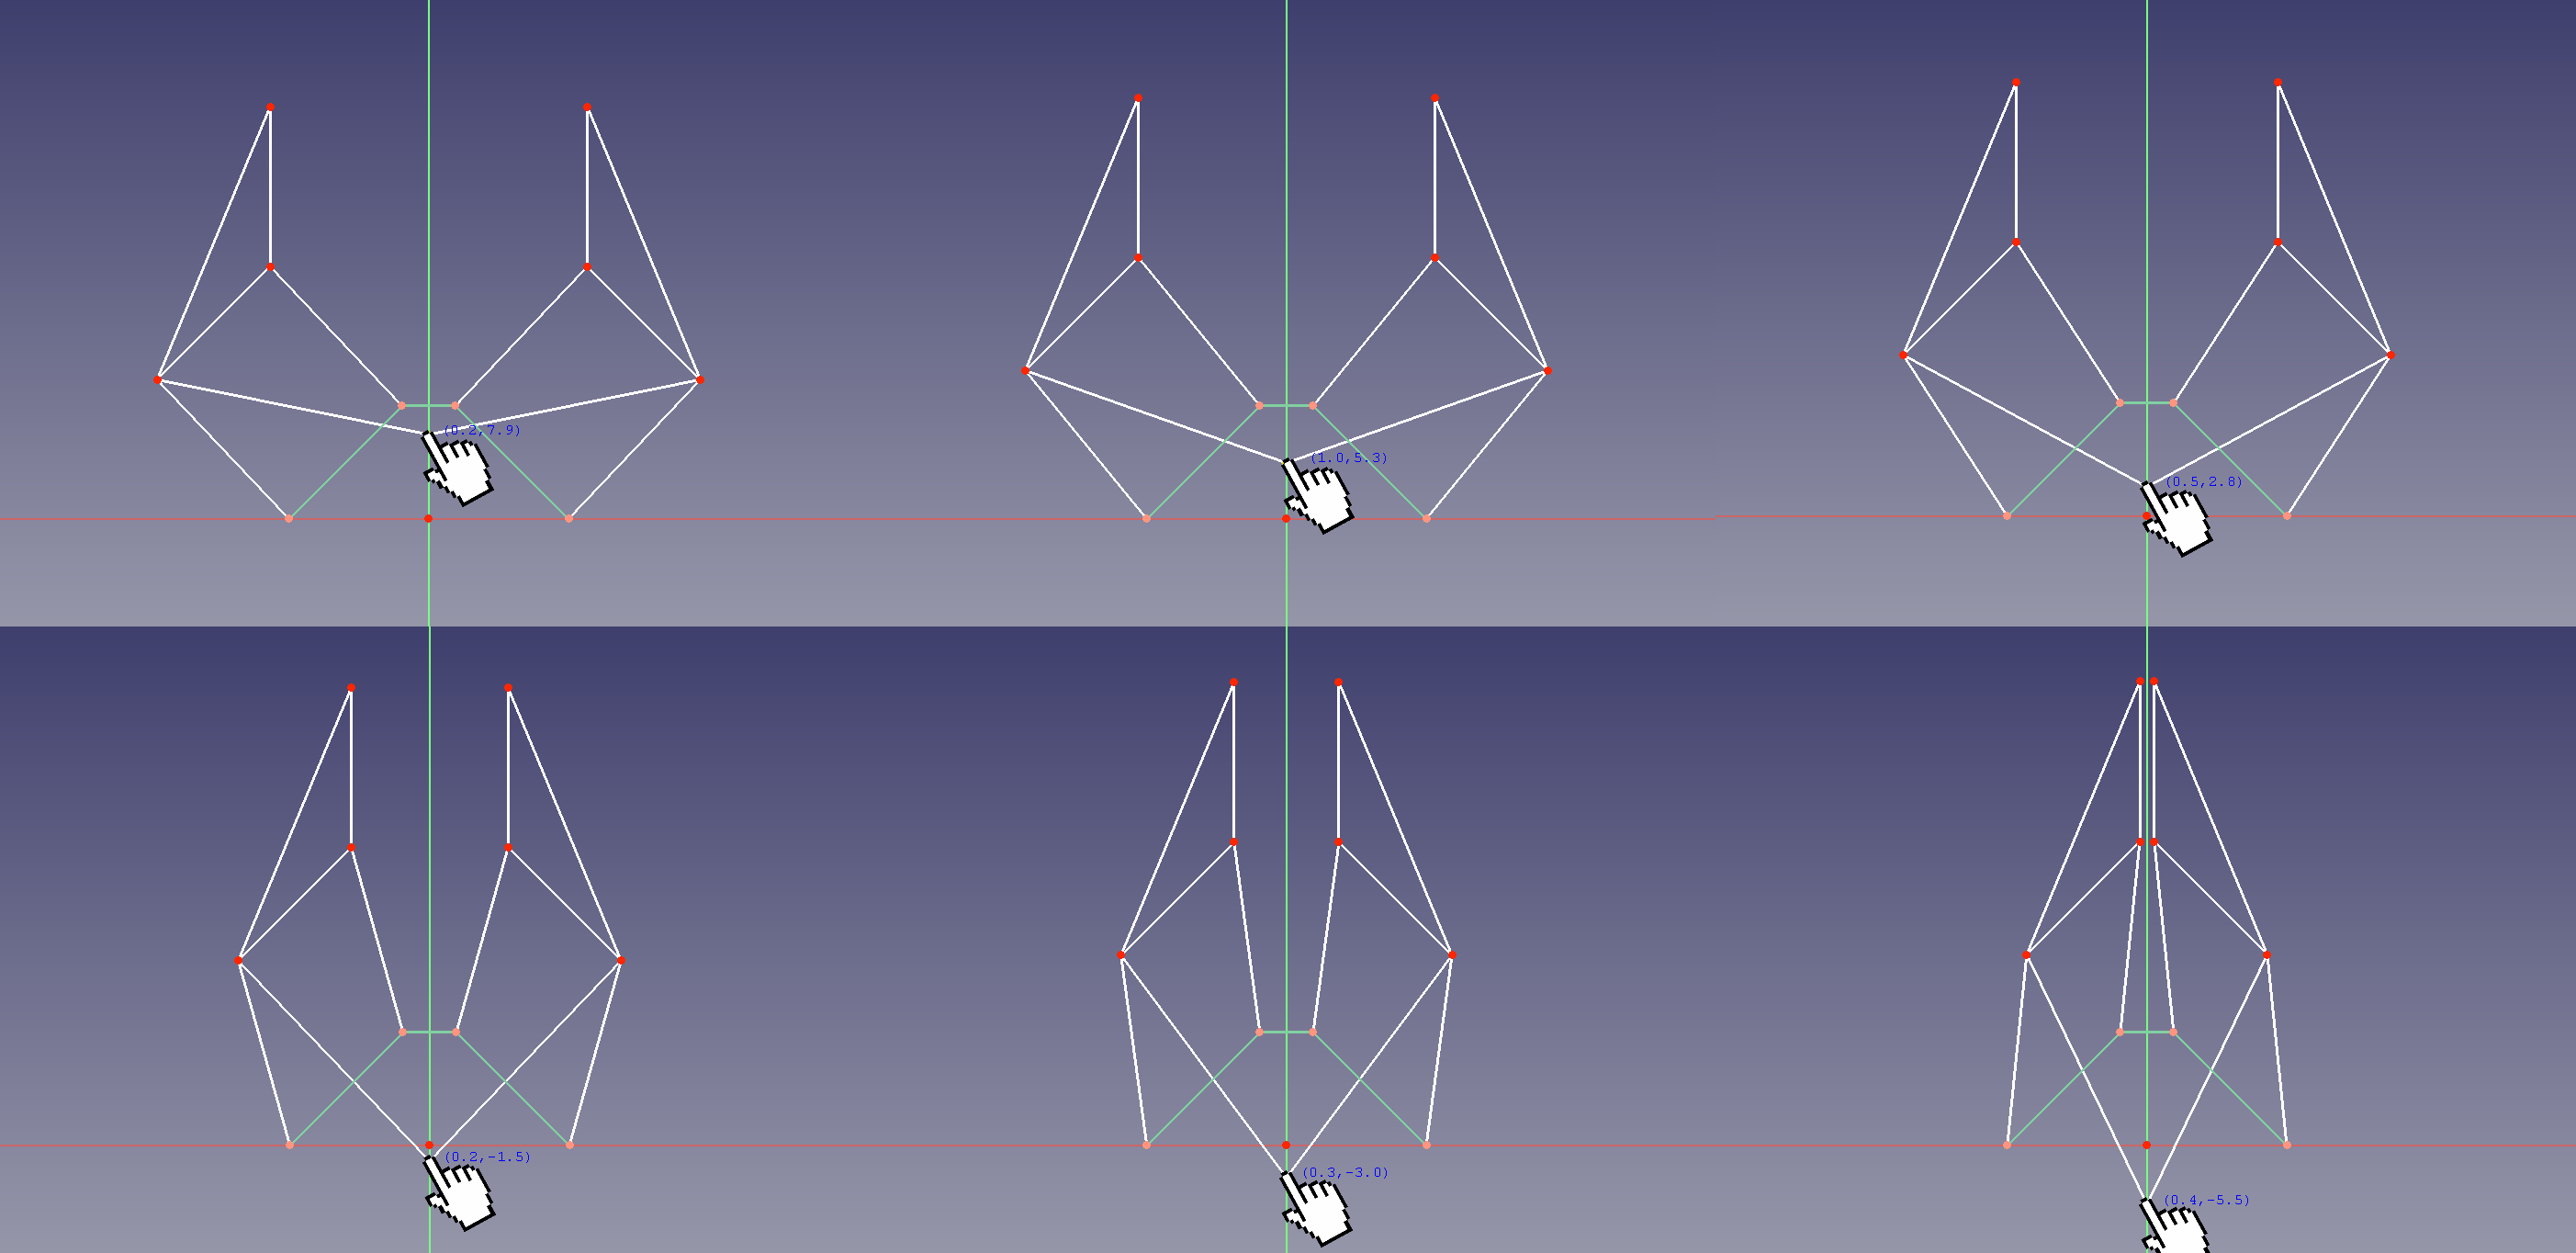
\includegraphics[width=15cm]{figs/pinza_evol.png}
  \end{center}
  \caption{Pinza paralela con 1 grado de libertad}
  \label{fig:mod_pinza_figure}
\end{figure}\ 

\subsection{Modelo alámbrico del brazo MeArm \ref{fig:mearm}}
\label{subsec:mod_mearm}


\section{Dinámica}

\section{DH}

\section{Bocetos}

\section{Diseño CAD}

\section{Diseño CAD}


\begin{code}[h]
\begin{lstlisting}[language=C++]
void Memory::hypothesizeParallelograms () {
  for(it1 = this->controller->segmentMemory.begin(); it1++) {
    squareFound = false; it2 = it1; it2++;
    while ((it2 != this->controller->segmentMemory.end()) && (!squareFound)) {
      if (geometry::haveACommonVertex((*it1),(*it2),&square)) {
        dist1 = geometry::distanceBetweenPoints3D ((*it1).start, (*it1).end);
        dist2 = geometry::distanceBetweenPoints3D ((*it2).start, (*it2).end);
      }
    // [...]
\end{lstlisting}
\caption[Función para buscar elementos 3D en la imagen]{Función para buscar elementos 3D en la imagen}
\label{cod:codejemplo}
\end{code}

En el Código \ref{cod:codejemplo2} vemos un ejemplo escrito en \texttt{Python}.

\begin{code}[h]
\begin{lstlisting}[language=Python]
def mostrarValores():
    print (w1.get(), w2.get())

master = Tk()
w1 = Scale(master, from_=0, to=42)
w1.pack()
w2 = Scale(master, from_=0, to=200, orient=HORIZONTAL)
w2.pack()
Button(master, text='Show', command=mostrarValores).pack()

mainloop()
\end{lstlisting}
\caption[Cómo usar un Slider]{Cómo usar un Slider}
\label{cod:codejemplo2}
\end{code}

\section{Verbatim}

Para mencionar identificadores usados en el código ---como nombres de funciones o variables--- en el texto, usa el entorno literal o verbatim \verb|hypothesizeParallelograms()|. También se puede usar este entorno para varias líneas, como se ve a continuación:

\begin{verbatim}
void Memory::hypothesizeParallelograms () {
  // add your code here
}
\end{verbatim}

\section{Ecuaciones}

Si necesitas insertar alguna ecuación, puedes hacerlo. Al igual que las figuras, no te olvides de referenciarlas. A continuación se exponen algunas ecuaciones de ejemplo: Ecuación \ref{ec:ec1} y Ecuación \ref{ec:ec2}.

\begin{myequation}[h]
\begin{equation}
H = 1 - \frac{\sum_{i=0}^{N}\frac{(\frac{d_{j_s} + d_{j_e}}{2})}{N}}{M}
\nonumber
\label{ec:ec1}
\end{equation}
\caption[Ejemplo de ecuación con fracciones]{Ejemplo de ecuación con fracciones}
\end{myequation} 

\begin{myequation}[h]
\begin{equation}
v(entrada)= \left\{
	\begin{array}{lcc}
		0 & \mbox{if} & \epsilon_t < 0.1\\
		K_p\cdot{(T_{t}-T)} & \mbox{if}& 0.1 \leq \epsilon_t < M_t\\
		K_p \cdot M_t & \mbox{if}& M_t < \epsilon_t
	\end{array}
\right.
\label{ec:ec2}
\end{equation}
\caption[Ejemplo de ecuación con array y letras y símbolos especiales]{Ejemplo de ecuación con array y letras y símbolos especiales}
\end{myequation}

\section{Tablas o cuadros}

Si necesitas insertar una tabla, hazlo dígnamente usando las propias tablas de \LaTeX, no usando pantallazos e insertándolas como figuras... En el Cuadro \ref{cuadro:ejemplo} vemos un ejemplo.

\begin{table}[H]
\begin{center}
\begin{tabular}{|c|c|}
\hline
\textbf{Parámetros} & \textbf{Valores} \\
\hline
Tipo de sensor & Sony IMX219PQ[7] CMOS 8-Mpx \\
Tamaño del sensor & 3.674 x 2.760 mm (1/4" format) \\
Número de pixels & 3280 x 2464 (active pixels) \\
Tamaño de pixel & 1.12 x 1.12 um \\
Lente & f=3.04 mm, f/2.0 \\
Ángulo de visión & 62.2 x 48.8 degrees \\
Lente SLR equivalente & 29 mm \\
\hline
\end{tabular}
\caption{Parámetros intrínsecos de la cámara}
\label{cuadro:ejemplo}
\end{center}
\end{table}



\chapter{Desarrollo software del manipulador}
\label{cap:capitulo6}

\vspace{1cm}
\noindent En este capítulo se aborda el desarrollo software necesario para poder usar el robot realizado 
tanto en simulaciones como en el mundo real.

\section{Control de los actuadores}
\noindent En esta sección se concretan los mecanismos y herramientas software utilizadas para poder controlar, desde 
un ordenador cualquiera, el hardware creado en el anterior capítulo.

\subsection{Grbl como \textit{firmware} del robot}
\noindent Para realizar el control de los actuadores se ha tomado la decisión de utilizar el 
firmware de control numérico Grbl (Sección \ref{subsec:grbl}), por encima 
de realizar uno propio, debido a que es una solución robusta con años de desarrollo y con unas ciertas garantías difíciles de superar.
\\
Actualmente, este firmware permite controlar hasta tres motores paso a paso simultáneamente. Además, tiene la posibilidad de utilizar 
un canal PWM (usualmente usado en las CNC para modificar la velocidad de la herramienta). Sobre estos motores, podemos realizar 
un control en posición, es decir, recibe una serie de coordenadas y automáticamente alcanza esos puntos. Este tipo de controlador 
es perfectamente válido para esta aplicación y simplifica bastante su uso. Aunque esta placa en concreto viene con Grbl 1.1 instalado 
de fábrica, existen numerosas guías en Internet acerca de como instalarlo.

Para que Grbl sepa qué posición debe tener cada motor en un momento dado, necesita recibir 
una serie de datos codificados a través de una de sus interfaces. Los detalles esta la comunicación 
se presentan en la siguiente subsección.
\newpage
\subsection{Comunicación con Grbl}
\noindent En esta sección se exponen las distintas opciones de comunicación con el robot, así como el formato de mensaje que se debe emplear.
\\ 
\indent Debido a las características hardware de la placa utilizada, se puede establecer comunicación con Grbl a través de 2 interfaces diferentes. 
La primera, es a través del propio puerto USB integrado, utilizando el protocolo serie UART. Este modo de comunicación tiene la ventaja de 
ser rápido pero te fuerza a estar conectado al robot a través de un cable. Por otro lado, debido a las características técnicas del 
microcontrolador, se puede establecer una comunicación inalámbrica a través de Wifi utilizando el protocolo Telnet. Finalmente, se ha optado 
por utilizar la interfaz USB debido a que es más rápida y permite al usuario estar conectado a internet, en vez de a la propia red 
\textit{offline} que crea la placa.

\indent Una forma de poder saber si viene ya instalado en la placa que hemos comprado, es utilizar una terminal serie, como 
puede ser \textit{Cutecom}. Establecemos una velocidad de 115200 baudios y nos conectamos al puerto que aparezca disponible 
al conectar la placa al ordenador. Si está instalado, veremos una serie de mensajes que indican la versión de Grbl y las 
distintas configuraciones internas. (Figura \ref{fig:cutecom})
\begin{figure} [ht!]
\begin{center}
    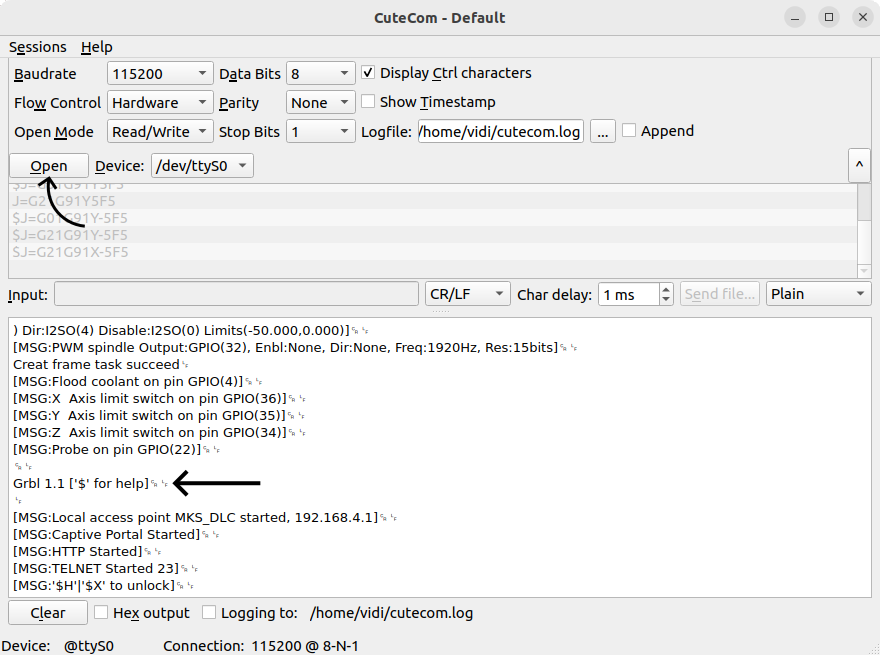
\includegraphics[width=14cm]{figs/cutecom.png}
\end{center}
\caption{Terminal gráfica de Cutecom al conectarse a una placa con Grbl}
\label{fig:cutecom}
\end{figure}

\indent Grbl recibe instrucciones de G-Code\ref{sec:gcode} a través del puerto serie. Aunque existen una gran 
cantidad de ellas, solo ha sido necesario usar algunas:
\begin{table}[H]
\begin{center}
\begin{tabular}{|l|l|}
\hline
\textbf{Comando} & \textbf{Explicación} \\
\hline
G92 X0 Y0 Z0 & G92 establece los valores de posición de cada eje\\
G01 & Establece que todos los ejes se moverán a la vez de forma lineal  \\
G90 X1 Y2 Z3 F34 & Mueve los motores a velocidad 34 hasta una coordenada absoluta  \\
S500 & Establece la velocidad del motor auxiliar a 500. Rango: 0-1000  \\
M3 & Enciende el motor auxiliar  \\
M5 & Apaga el motor auxiliar  \\
? & Recibir el estado actual de la maquina  \\
! & Para el movimiento actual \\
\textasciitilde & Continua con el movimiento parado anteriormente \\
\hline
\end{tabular}
\caption{Comandos utilizados en la realización del proyecto}
\end{center}
\end{table}


Con el objetivo de abstraer al futuro software del robot de esta comunicación, se ha implementado 
una clase en Python\ref{subsec:pyhton} llamada \textit{Grbl}. En este software, utiliza la librería 
PySerial\footnote{\url{https://pypi.org/project/pyserial/}} para establecer una comunicación 
serie. La clase \textit{Grbl} creada puede ser utilizada a través de los métodos mostrados en el Código \ref{code:grblapi}. Y su 
código fuente puede ser encontrado en el repositorio del 
proyecto\footnote{\url{https://github.com/RoboticsURJC/tfg-vperez/blob/96fc1e44bef6a31c272fb0673b5a33a7571c5ee7/src/software/g_arm/g_arm/g_arm_lib/grblAPI.py}}.
\\
\begin{code}[h]
\begin{lstlisting}[language=Python,  literate={á}{{\'a}}1 {é}{{\'e}}1 {í}{{\'i}}1 {ó}{{\'o}}1 {ú}{{\'u}}1 {ñ}{{\~n}}1]
start(puerto) # Devuelve true/false en función de si ha sido posible conectarse
stop() # Finaliza la comunicación
setSpindleSpeed(value) # Establece la velocidad del motor auxiliar
enableSpindle() # Activa el motor auxiliar
disableSpindle() # Desactiva el motor auxiliar
setCoordinates(x, y, z) # Establece las coordenadas x, y, z 
getXYZ() # Devuelve la posición actual
asyncXYZMove(posición, velocidad, relative) # Mueve los motores a una posición con la velodicad dada. Permite realizar movimientos relativos y absolutos.
\end{lstlisting}
\caption{API de la clase \textit{Grbl}}
\label{code:grblapi}
\end{code}


A pesar de que ya podemos comandar movimientos en los distintos ejes de la máquina, se requiere realizar una serie 
de configuraciones para definir las características concretas de cada articulación.
\newpage
\subsection{Configuración de Grbl para su uso en robótica}
\noindent Grbl tiene ciertas limitaciones a la hora de usarse en robótica. Es normal, debido a que está pensado para controlar máquinas 
\acs{CNC} de 3 ejes prismáticos. Pese a esto, se pueden unas ciertas configuraciones para adaptarlo a esta aplicación. 

\subsubsection{Parámetros de Grbl}
Este \textit{firmware} guarda en su memoria interna una serie de parámetros que definen su 
comportamiento. Si se quiere visualizar cuáles son y sus respectivos valores, hay que enviar 
el mensaje \textbf{\$\$} a través del puerto serie. Para modificar un cierto valor, hay que introducir una cadena 
con el formato: \textbf{\$identificador del parámetro=nuevoValor}.

Para modificar la configuración de una forma cómoda, se recomienda utilizar herramientas como 
\textit{UniversalGcodeSender} (Figura \ref{fig:ugs}).

\begin{figure} [ht!]
\begin{center}
    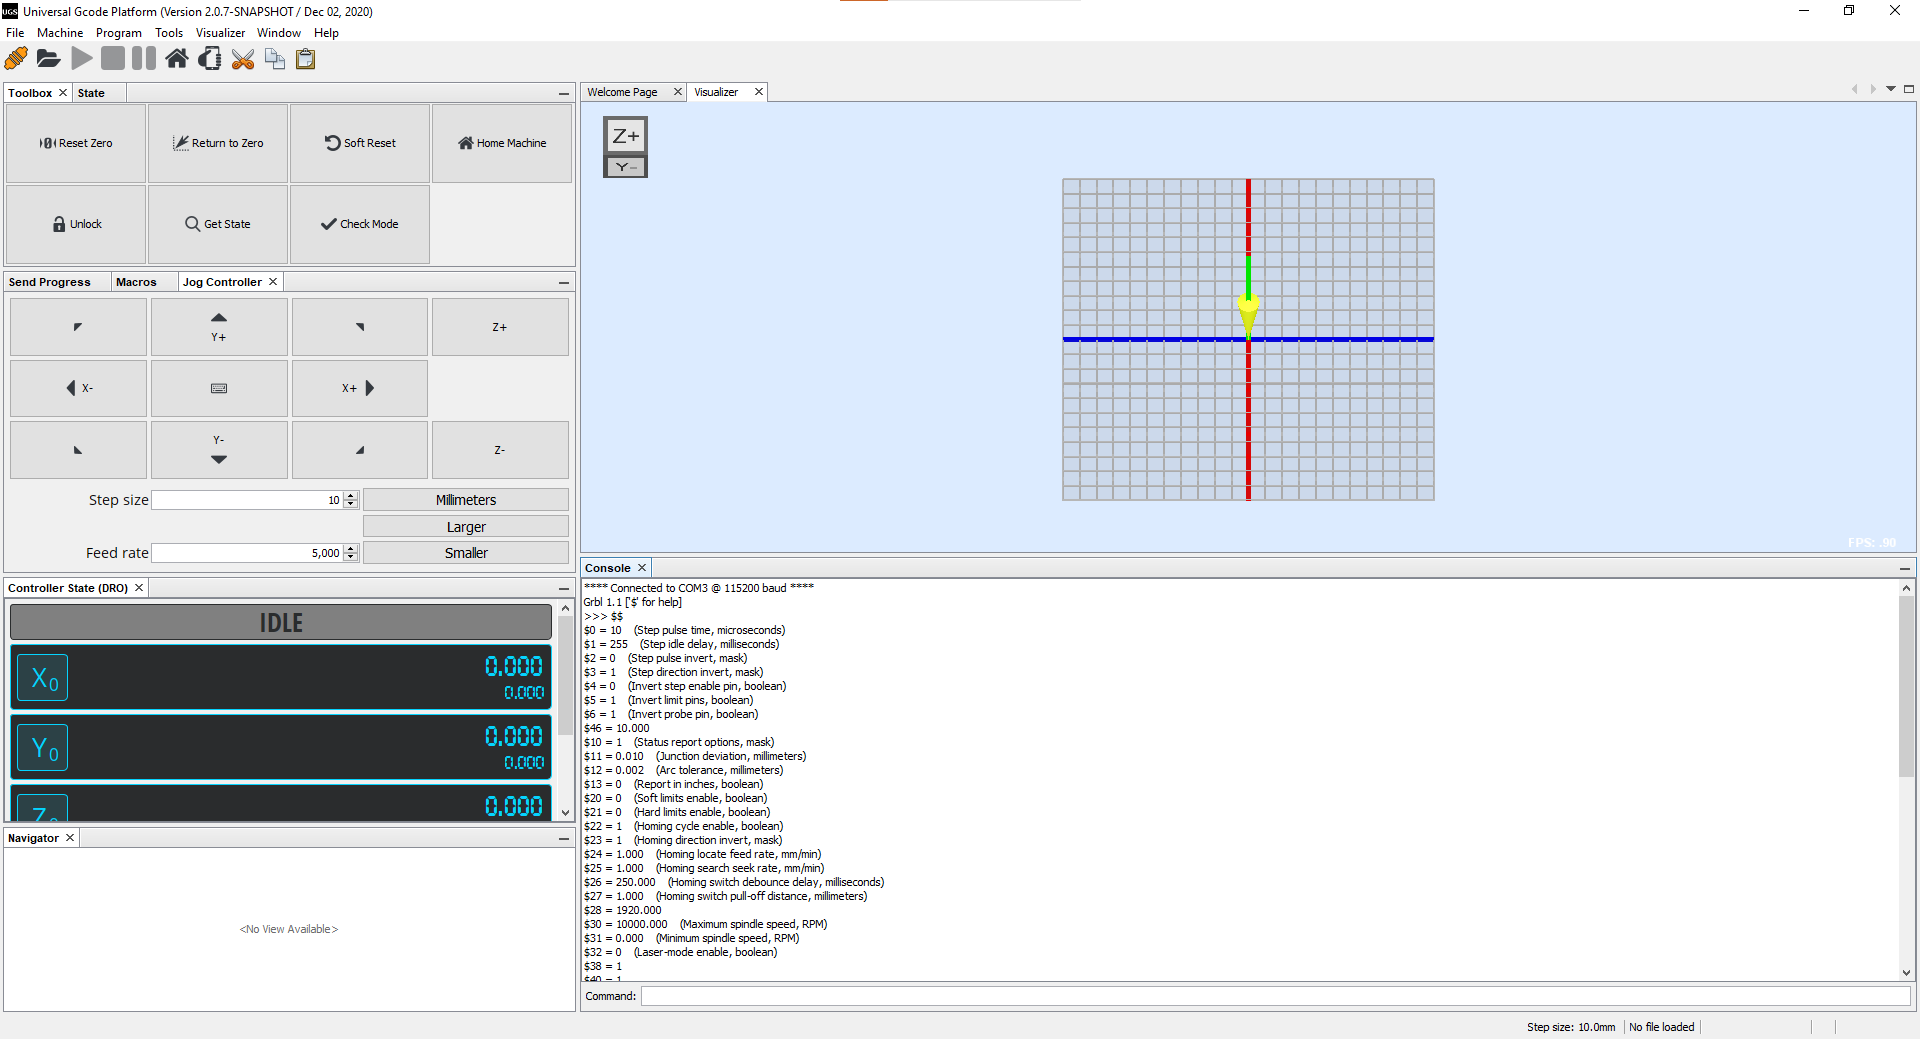
\includegraphics[width=15cm]{figs/ugs.png}
\end{center}
\caption{Interfaz de UniversalGcodeSender\footnote{\url{https://winder.github.io/ugs_website/download/}}}
\label{fig:ugs}
\end{figure}

Puesto que se quiere utilizar Grbl para controlar un brazo robot, debemos 
realizar las siguientes configuraciones:
\begin{itemize}
\item \textbf{\$1}: Retardo o tiempo de espera entre pulsos de paso cuando el motor está inactivo (en milisegundos). 
\\Debemos configurar 
este parámetro en su valor máximo, en este caso 255. Este valor tiene un significado especial, haciendo que los motores paso a paso 
se mantengan energizados constantemente aunque no se estén moviendo. Es de vital importancia para evitar que el brazo se desplome al detenerse en una cierta posición.  
\item \textbf{\$100}, \textbf{\$101} y \textbf{\$102}: Indican el número de pasos por unidad de movimiento para los ejes X, Y, Z respectivamente. 
\\Por defecto está pensado para utilizar pasos por milímetro. Como se pretende utilizar articulaciones de rotación, debemos expresar esta relación 
en función de alguna medida angular. La unidad a utilizar podría ser: grados, radianes o vueltas, entre otras. En este trabajo se 
utilizan los grados debido a que en radianes y vueltas la unidad correspondía a un gran número de pasos y era difícil controlar la aceleración para incrementos de 
0.1 vueltas. 

\begin{myequation}[h!]
\begin{equation}
    PasosPorGrado = \frac{Microstepping * Ratio}{1.8^\circ}
\nonumber
\label{ec:pasos_por_grado}
\end{equation}
\caption[Cálculo de pasos por grado en Grbl]{Cálculo de pasos por grado en Grbl}
\end{myequation} 

\item \textbf{\$110}, \textbf{\$111} y \textbf{\$112}: Indican la velocidad máxima a la que puede moverse cada eje X, Y, Z en unidades por segundo. 
En este caso, grados por segundo. Estos valores se deben encontrar por medio de la experimentación. Se trata de una medida de seguridad en 
caso de que el usuario quiera mover demasiado rápido un eje pudiendo dañar el brazo.

\item \textbf{\$120}, \textbf{\$121} y \textbf{\$122}: Indican la aceleración máxima a la que puede moverse cada eje X, Y, Z en unidades por segundo cuadrado. 
En este caso, grados por segundo cuadrado. Estos valores también se deben encontrar por medio de la experimentación. Se trata de una medida de seguridad en 
caso de que el usuario quiera mover demasiado rápido un eje pudiendo dañar el brazo. Se debe encontrar una aceleración idónea para todos 
los movimientos, una limitación de grbl es que no se puede comandar un movimiento diciéndole una determinada aceleración.
\end{itemize}

Para profundizar más en la finalidad de cada parámetro, código y configuración se 
recomienda leer la documentación \footnote{\url{https://github.com/gnea/grbl/blob/master/doc/markdown/commands.md}}
\footnote{\url{https://github.com/gnea/grbl/blob/master/doc/markdown/settings.md}}
\\
\newpage
En el caso concreto de este proyecto, se ha utilizado la configuración mostrada en la Tabla \ref{cuadro:parametros_grbl}.
\\

\begin{table}[H]
\begin{center}
\begin{tabular}{|c|c|}
\hline
\textbf{Parámetro} & \textbf{Valor} \\
\hline
\textdollar0 & $10$ \quad (Step pulse time, microseconds) \\
\textdollar1 & $255$ \quad (Step idle delay, milliseconds) \\
\textdollar2 & $0$ \quad (Step pulse invert, mask) \\
\textdollar3 & $1$ \quad (Step direction invert, mask) \\
\textdollar4 & $0$ \quad (Invert step enable pin, boolean) \\
\textdollar5 & $1$ \quad (Invert limit pins, boolean) \\
\textdollar6 & $1$ \quad (Invert probe pin, boolean) \\
\textdollar10 & $1$ \quad (Status report options, mask) \\
\textdollar11 & $0.010$ \quad (Junction deviation, millimeters) \\
\textdollar12 & $0.002$ \quad (Arc tolerance, millimeters) \\
\textdollar13 & $0$ \quad (Report in inches, boolean) \\
\textdollar20 & $0$ \quad (Soft limits enable, boolean) \\
\textdollar21 & $0$ \quad (Hard limits enable, boolean) \\
\textdollar22 & $1$ \quad (Homing cycle enable, boolean) \\
\textdollar23 & $1$ \quad (Homing direction invert, mask) \\
\textdollar24 & $1.000$ \quad (Homing locate feed rate, mm/min) \\
\textdollar25 & $1.000$ \quad (Homing search seek rate, mm/min) \\
\textdollar26 & $250.000$ \quad (Homing switch debounce delay, milliseconds) \\
\textdollar27 & $1.000$ \quad (Homing switch pull-off distance, millimeters) \\
\textdollar30 & $10000.000$ \quad (Maximum spindle speed, RPM) \\
\textdollar31 & $0.000$ \quad (Minimum spindle speed, RPM) \\
\textdollar32 & $0$ \quad (Laser-mode enable, boolean) \\
\textdollar100 & $26.666$ \quad (X-axis travel resolution, step/mm) \\
\textdollar101 & $22.222$ \quad (Y-axis travel resolution, step/mm) \\
\textdollar102 & $22.222$ \quad (Z-axis travel resolution, step/mm) \\
\textdollar110 & $6000.000$ \quad (X-axis maximum rate, mm/min) \\
\textdollar111 & $6000.000$ \quad (Y-axis maximum rate, mm/min) \\
\textdollar112 & $6000.000$ \quad (Z-axis maximum rate, mm/min) \\
\textdollar120 & $60.000$ \quad (X-axis acceleration, mm/sec\textasciicircum2) \\
\textdollar121 & $60.000$ \quad (Y-axis acceleration, mm/sec\textasciicircum2) \\
\textdollar122 & $60.000$ \quad (Z-axis acceleration, mm/sec\textasciicircum2) \\
\textdollar130 & $450.000$ \quad (X-axis maximum travel, millimeters) \\
\textdollar131 & $450.000$ \quad (Y-axis maximum travel, millimeters) \\
\textdollar132 & $50.000$ \quad (Z-axis maximum travel, millimeters) \\
\end{tabular}
\caption{Parámetros Grbl usados en este trabajo}
\label{cuadro:parametros_grbl}
\end{center}
\end{table}

\newpage
\section{Integración con ROS 2}
\noindent En esta sección se detalla el proceso de integración del robot G-Arm en \acs{ROS}, pasando 
por la creación de la descripción, la visualización, la configuración y la simulación. 

\subsection{Descripción del robot}
\noindent El primer paso en la integración de un robot en el ecosistema ROS, es lograr expresar 
su forma y funcionamiento de tal manera que pueda ser visualizado, simulado y controlado en el mundo 
virtual. Esto es conocido como describir un robot y para ello existen diferentes formatos entre los que destacan URDF y Xacro.

\subsubsection{Creación del paquete de descripción}
\noindent Para crear el paquete, se ha seguido el siguiente
\begin{enumerate}
    \item En el \textit{src} del workspace ejecutamos:
    \begin{verbatim}
        ros2 pkg create --build-type ament_cmake g_arm_description
    \end{verbatim}   
    \item Dentro de la carpeta que se ha generado, creamos 3 nuevos directorios:
    \begin{verbatim}
        mkdir launch rviz urdf meshes
    \end{verbatim} 
        
    \item Añadimos al fichero \textit{package.xml}: 
    \lstset{
        language=XML, % Establece el lenguaje como XML
        basicstyle=\ttfamily, % Fuente monoespaciada
        keywordstyle=\bfseries\color{blue}, % Estilo de las palabras clave
        commentstyle=\itshape\color{gray}, % Estilo de los comentarios
        stringstyle=\color{orange}, % Estilo de las cadenas de texto
        showstringspaces=false, % No mostrar espacios en cadenas de texto
        breaklines=true, % Dividir líneas largas
        frame=lines, % Agregar un marco alrededor del código
        numbers=left, % Mostrar números de línea
        numberstyle=\tiny\color{gray}, % Estilo de los números de línea
        captionpos=b % Posición de la leyenda del código (abajo)
    }
    
    \begin{lstlisting}
        <exec_depend>joint_state_publisher</exec_depend>
        <exec_depend>robot_state_publisher</exec_depend>
        <exec_depend>rviz</exec_depend>
        <exec_depend>xacro</exec_depend>
    \end{lstlisting}
    
    \item Compilamos el paquete desde la raíz del workspace:
    \begin{verbatim}
        colcon build --symlink-install
    \end{verbatim}
    \item Añadimos la siguiente línea al final del .bashrc para que ROS pueda encontrar el paquete:
    \begin{verbatim}
        source ~/workspace/install/local_setup.bash
    \end{verbatim}
    
    \end{enumerate}

\subsubsection{Describir un robot mediante URDF y Xacro}
\ac{URDF} es un formato de archivo cuyo propósito es describir la estructura, cinemática y aspecto de un robot.  
Se trata de un estándar ampliamente utilizado en la comunidad robótica, especialmente en \ac{ROS}.

En este tipo de archivo, se especifica la geometría del robot mediante la definición de eslabones (links) 
y articulaciones (joints). 
Cada eslabón es descrito por su aspecto y geometría, mientras que las articulaciones están definidas
en cuanto a su tipo, recorrido y posición. Además de esto, un archivo URDF puede incluir información 
sobre la masa y la inercia de los eslabones, así como como texturas y modelos 3D.

\begin{figure} [ht!]
    \begin{center}
        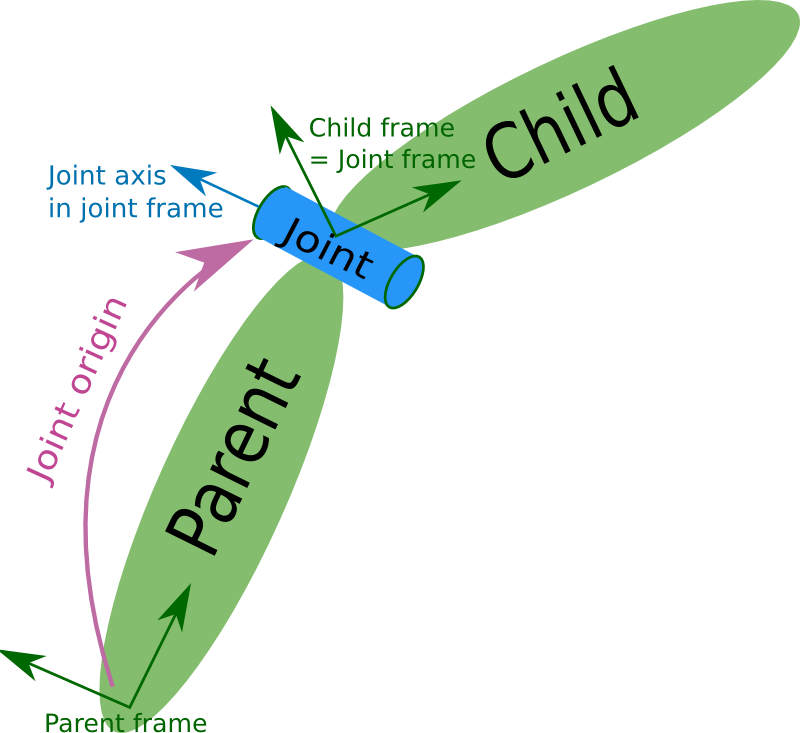
\includegraphics[width=10cm]{figs/urdf.png}
    \end{center}
    \caption{Elementos del formato URDF\footnote{\url{http://library.isr.ist.utl.pt/docs/roswiki/urdf\%282f\%29XML\%282f\%29Joint.html}}}
\label{fig:urdf}
\end{figure}
Este formato se basa en el lenguaje \ac{XML}, lo que permite describir el robot de una forma 
estructurada y legible. Por otro lado, Xacro es un lenguaje de macros XML que simplifica la 
creación de descripciones URDF al permitir la reutilización de código y la parametrización 
de modelos. Se puede convertir un fichero Xacro a URDF ejecutando el siguiente comando:
\begin{verbatim}
    xacro fichero.xacro > fichero.urdf
\end{verbatim}
\newpage
Con el objetivo de lograr una descripción lo más realista posible, se han empleado las mismas geometrías del diseño \acs{CAD}.
Para poder incluirlas en el URDF, es necesario exportar las piezas al formato \textit{Collada} (.dae) desde FreeCAD. Este formato 
contiene información acerca de la geometría, posición, tamaño y colores, de la pieza en cuestión.
\\
Además del aspecto visual, hay que definir el volumen físico que ocupan en el espacio. Las mallas de colisión son la representación 
geométrica simplificada utilizada para calcular interacciones físicas y detectar colisiones en simulaciones. En este caso se va a utilizar 
un formato muy liviano de malla, el \ac{STL}. 

Tanto los ficheros Collada como los ficheros STL, deben estar en la carpeta \textit{meshes} creada anteriormente. En cambio; el fichero 
URDF debe estar en la carpeta \textit{urdf}.
\\

Un aspecto a tener en cuenta, es que no todos los tipos de robot pueden ser descritos con este formato. La limitación radica en que 
un eslabón hijo solo soporta un eslabón padre, por lo que no se pueden construir cadenas cinemáticas cerradas. \\
\begin{figure} [ht!]
    \centering  
    \subfigure[Cerrada]{\label{fig:abierta}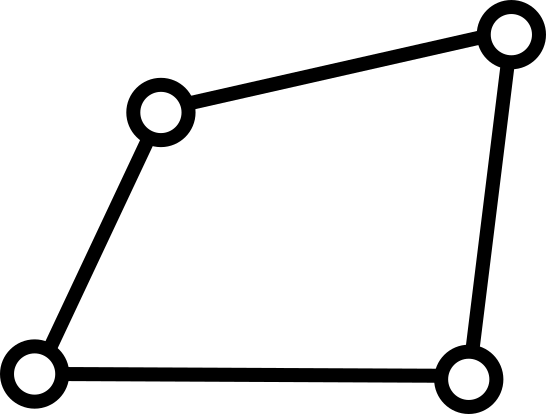
\includegraphics[width=0.3\linewidth ]{figs/cerrada.png}}
    \hspace{2cm}
    \subfigure[Abierta]{\label{fig:cerrada}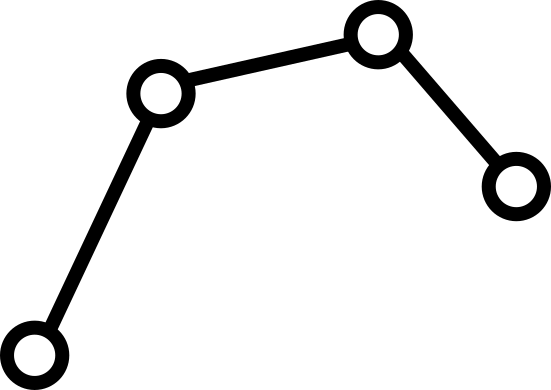
\includegraphics[width=0.3\linewidth ]{figs/abierta.png}}
    \caption{Cadenas cinemáticas}
  \end{figure}\ 
\\
El robot de este trabajo esta constituido enteramente por cadenas cinemáticas cerradas. Pese a esto, se ha utilizado el ingenio y un tipo de 
articulación específico para lograr describir este tipo de robot de forma exacta. Se llama \textit{Mimic joint} y
es un tipo de articulación pasiva que imita el ángulo de otra. Con una cierta combinación de varias de ellas, y una serie de 
eslabones invisibles se puede lograr describir este tipo de robot. 
Además, ha sido necesario añadir una cuarta articulación \enquote{falsa}. Esta indica la intensidad del electroimán acoplado al robot. 
Es de tipo revolución, pero su recorrido es de 0.001 radianes por lo que apenas afecta a la cinemática. 

El fichero\footnote{\url{https://github.com/RoboticsURJC/tfg-vperez/blob/8d3b281d701ec4a57602a9dcfcdd04888955319b/src/software/g_arm_description/urdf/robot_electromagnet.urdf}} 
URDF final puede ser encontrado junto al resto del proyecto en el repositorio de Git.
\newpage
\subsubsection{Creación de un launcher para visualizar el robot}
\noindent Para visualizar el fichero que hemos creado anteriormente, podemos realizar una herramienta de ROS 
llamada RViz. Esta herramienta no solo permite visualizar, sino también analizar datos de sensores, modelos de robot y 
planificaciones de movimiento de forma interactiva. Además se le pueden añadir complementos para agregarle funcionalidades extra. 
\\

Para que se pueda cargar la descripción del robot en este visualizador, debe haber algo que la esté publicando en el topic 
\textit{robot\_description}. Es por esto que existe un nodo de ROS llamado \textit{robot\_state\_publisher} que se encarga 
de ello. Además, si queremos algo más que una representación estática, podemos utilizar un nodo llamado \mbox{\textit{joint\_state\_publisher\_gui}}. Este nodo 
muestra una ventana gráfica con una serie de controles para controlar manualmente cada joint. 
\\

Teniendo en cuenta que se requiere lanzar una serie de nodos y programas, es útil crear un \textit{launcher} de ROS. Un \textit{launcher} es una 
herramienta que se utiliza para iniciar, configurar, gestionar y desplegar nodos. Este tipo de fichero terminado en 
\textit{.launch.py} se almacenan en la carpeta \textit{launch}. Para crearlo, se ha usado como inspiración el lanzador \textit{visualize\_franka.launch.py} del 
robot Franka Emika\footnote{\url{https://github.com/frankaemika/franka_ros2/blob/develop/franka_description/launch/visualize_franka.launch.py}}.
\\

Finalmente, el paquete de descripción está terminado. Ejecutando el siguiente comando, se nos abrirá una ventana de RViz y una 
serie de controles deslizantes para cada articulación (Figura \ref{fig:rviz}).
\begin{verbatim}
    ros2 launch g_arm_description display_tool.launch.py
\end{verbatim}

\begin{figure} [ht!]
    \begin{center}
        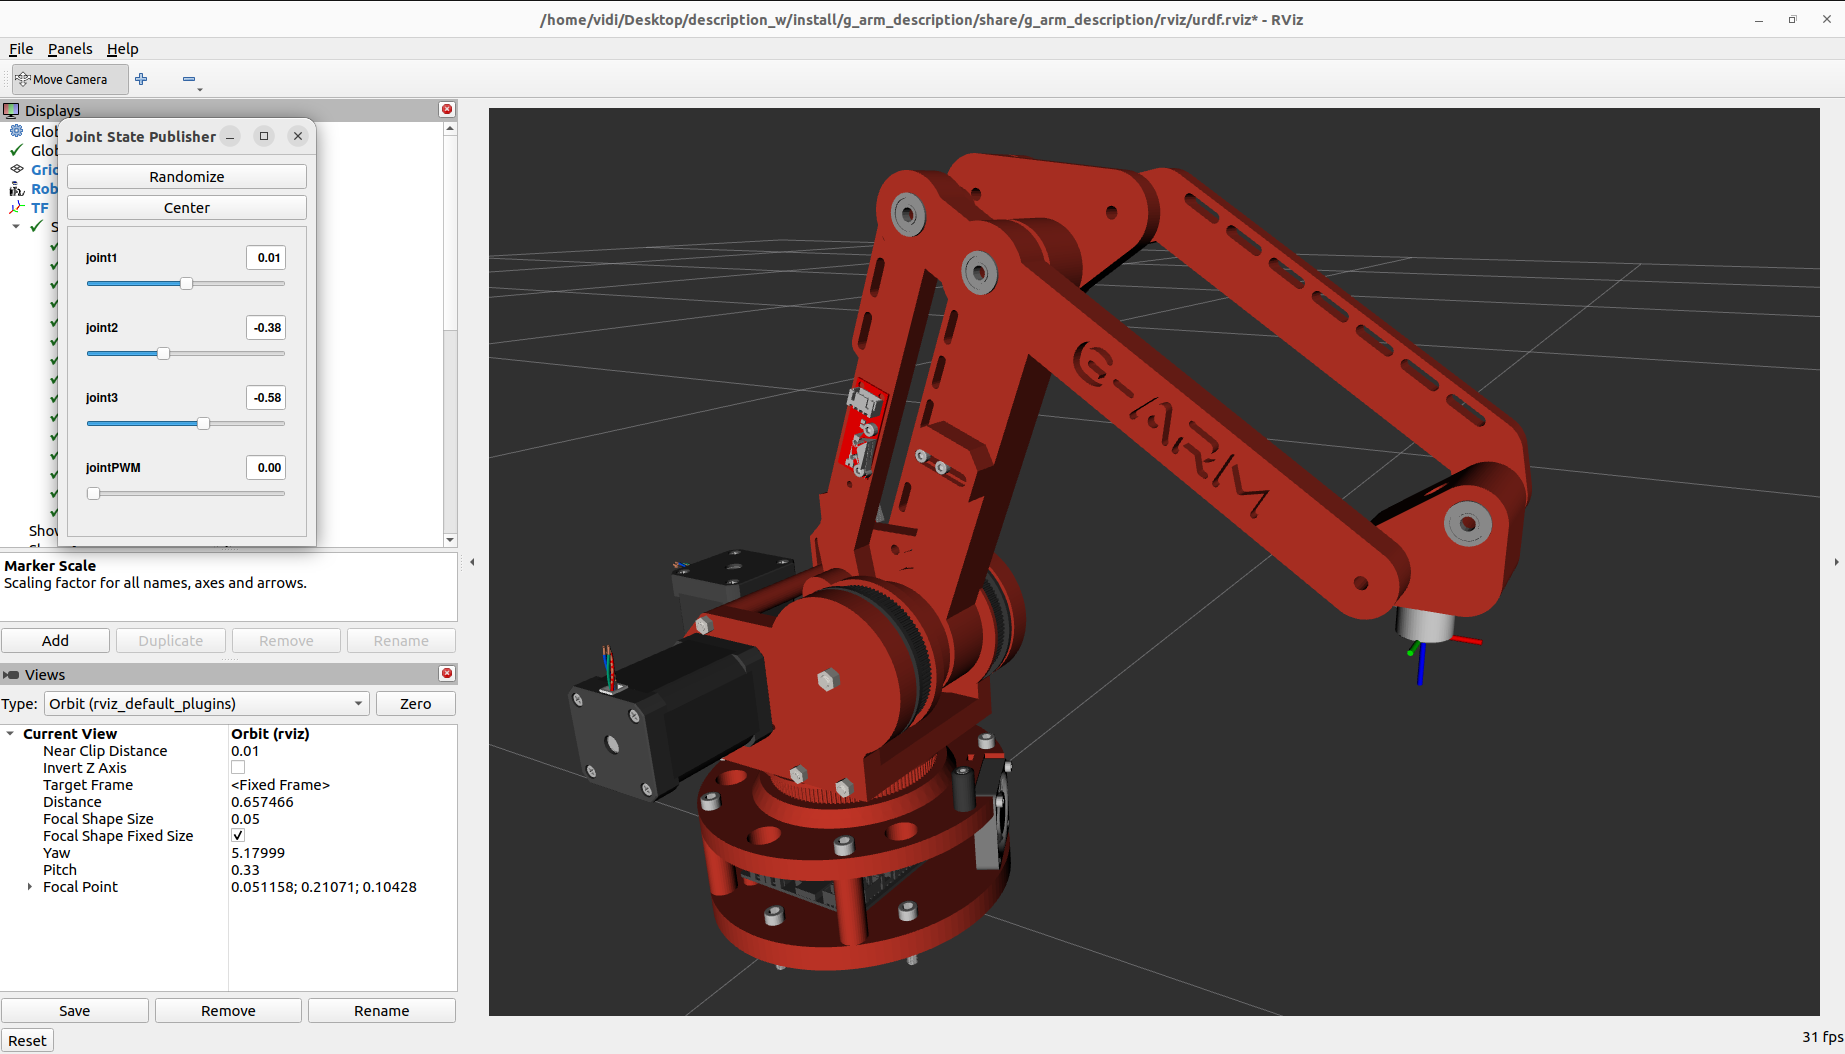
\includegraphics[width=15cm]{figs/RViz.png}
    \end{center}
    \caption{Ventana de RViz visualizado el robot creado}
\label{fig:rviz}
\end{figure}

\newpage
\subsection{Integración con MoveIt 2}
\noindent En esta sección se enumeran y describen los pasos necesarios para, a partir de un paquete de descripción de un robot, generar 
un paquete de MoveIt.
\\
Antes de comenzar, debemos tener instalado MoveIt 2 para ROS Humble. Para ello, se ha seguido el proceso de 
instalación\footnote{\url{https://moveit.picknik.ai/main/doc/tutorials/getting_started/getting_started.html}} de la documentación.
\\

Para crear el paquete de MoveIt de este robot, se han llevado a cabo los siguientes pasos:
\begin{enumerate}
\item Lanzamos el asistente de configuración.
\begin{verbatim}
    ros2 launch moveit_setup_assistant setup_assistant.launch.py
\end{verbatim}
\item Pulsamos sobre \textbf{\textit{\guillemotleft Create New MoveIt Configuration Package\guillemotright}} y cargamos el URDF/Xacro del paquete de descripción 
del robot. Si el fichero es válido, aparecerán una serie de apartados a configurar en el lateral izquierdo del asistente. 
\item Comenzamos configurando la apartado \textbf{\textit{\guillemotleft Self-Collisions\guillemotright}}. Aquí se hace uso de la colisiones 
descritas anteriormente para generar una matriz de posibles colisiones que se pueden dar. Para ello, pulsamos sobre
\textbf{\textit{\guillemotleft Generate Collision Matrix\guillemotright}}.
\item Acto seguido se configura el apartado \textbf{\textit{\guillemotleft Planning Groups\guillemotright}}, donde se establecen los eslabones y articulaciones que serán consideradas 
a la hora de realizar la planificación. Para ello, pulsamos sobre \textbf{\textit{\guillemotleft Add Group\guillemotright}} y acto seguido 
le damos un nombre. Posteriormente, pulsamos sobre \textbf{\textit{\guillemotleft Add Kin. Chain\guillemotright}} y seleccionamos como 
eslabón base, el eslabón que irá unido al suelo, y como eslabón \textit{tip}, el extremo del robot (sin llegar a la herramienta). Entonces, guardamos los cambios. Ahora, 
se añaden todos los \textit{links} y \textit{joints} de la cadena anterior, al grupo de planificación creado, dando en \textbf{\textit{\guillemotleft Edit Selected\guillemotright}}.
Repetimos este procedimiento con el grupo de planificación de la herramienta, seleccionando como eslabón base el eslabón final de la anterior cadena, y como 
final de esta, el último eslabón de la herramienta. 

\item En el apartado \textbf{\textit{\guillemotleft Robot Poses\guillemotright}} se pueden configurar una serie de posiciones predeterminadas 
para poder usarse posteriormente cuando se necesiten. Por ejemplo, es recomendable crear al menos dos; una que haga de posición \textit{Home} 
(Posición cómoda para empezar a trabajar) y otra como posición de reposo (Posición que evita que el robot se desplome al cortar la electricidad). Además 
podemos añadir dos más para el grupo de planificación de la herramienta: \textit{ToolON} y \textit{ToolOFF}.

\item Usamos el apartado \textbf{\textit{\guillemotleft End Effectors \guillemotright}} para configurar el extremo de nuestro robot como tal. Para ello, 
seleccionamos el eslabón del extremo y el grupo de planificación creado anteriormente. 

\item En \textbf{\textit{\guillemotleft Passive Joints\guillemotright}}, añadimos todos aquellas articulaciones que no sean grados de libertad, 
es decir, todas aquellas que no sean \textit{joint1, joint2, joint3, jointPWM (señal PWM de la herramienta)}.

\item En los apartados \textbf{\textit{\guillemotleft ROS 2 Controllers\guillemotright}} y 
\textbf{\textit{\guillemotleft MoveIt Controllers\guillemotright}}, añadimos automáticamente los controladores pulsando sobre el único botón que hay.

\item Finalmente rellenamos nuestra información personal en \textbf{\textit{\guillemotleft Author information\guillemotright}} y generamos el 
paquete en el \textit{src} del \textit{workspace}. Acto seguido, compilamos.
\end{enumerate}

A la hora de usar esta herramienta, se debe de tener en cuenta que a día de la publicación de este trabajo, existe un error en el asistente
que hace que el paquete no se cree bien del todo. Para corregirlo, es necesario cambiar todos los número del fichero \textit{joints\_limits.yaml}
del paquete generado a \textit{double}. Es decir, cambiar por ejemplo un ``200" por ``200.0".
\\
\newpage
Para comprobar que el paquete ha sido configurado bien, ejecutamos un \textit{launcher} generado automáticamente por el asistente :
\begin{verbatim}
    ros2 launch g_arm_moveit demo.launch.py
\end{verbatim}
Tras ejecutarlo, se debería abrir una ventana de RViz con un aspecto similar a lo mostrado en la Figura \ref{fig:moveit_demo}. Podemos utilizar 
el propio \textit{plugin} de MoveIt para establecer una posición aleatoria y tratar de llegar a ella (Figura \ref{fig:moveit_trayectory_demo}).
\begin{figure} [ht!]
    \begin{center}
      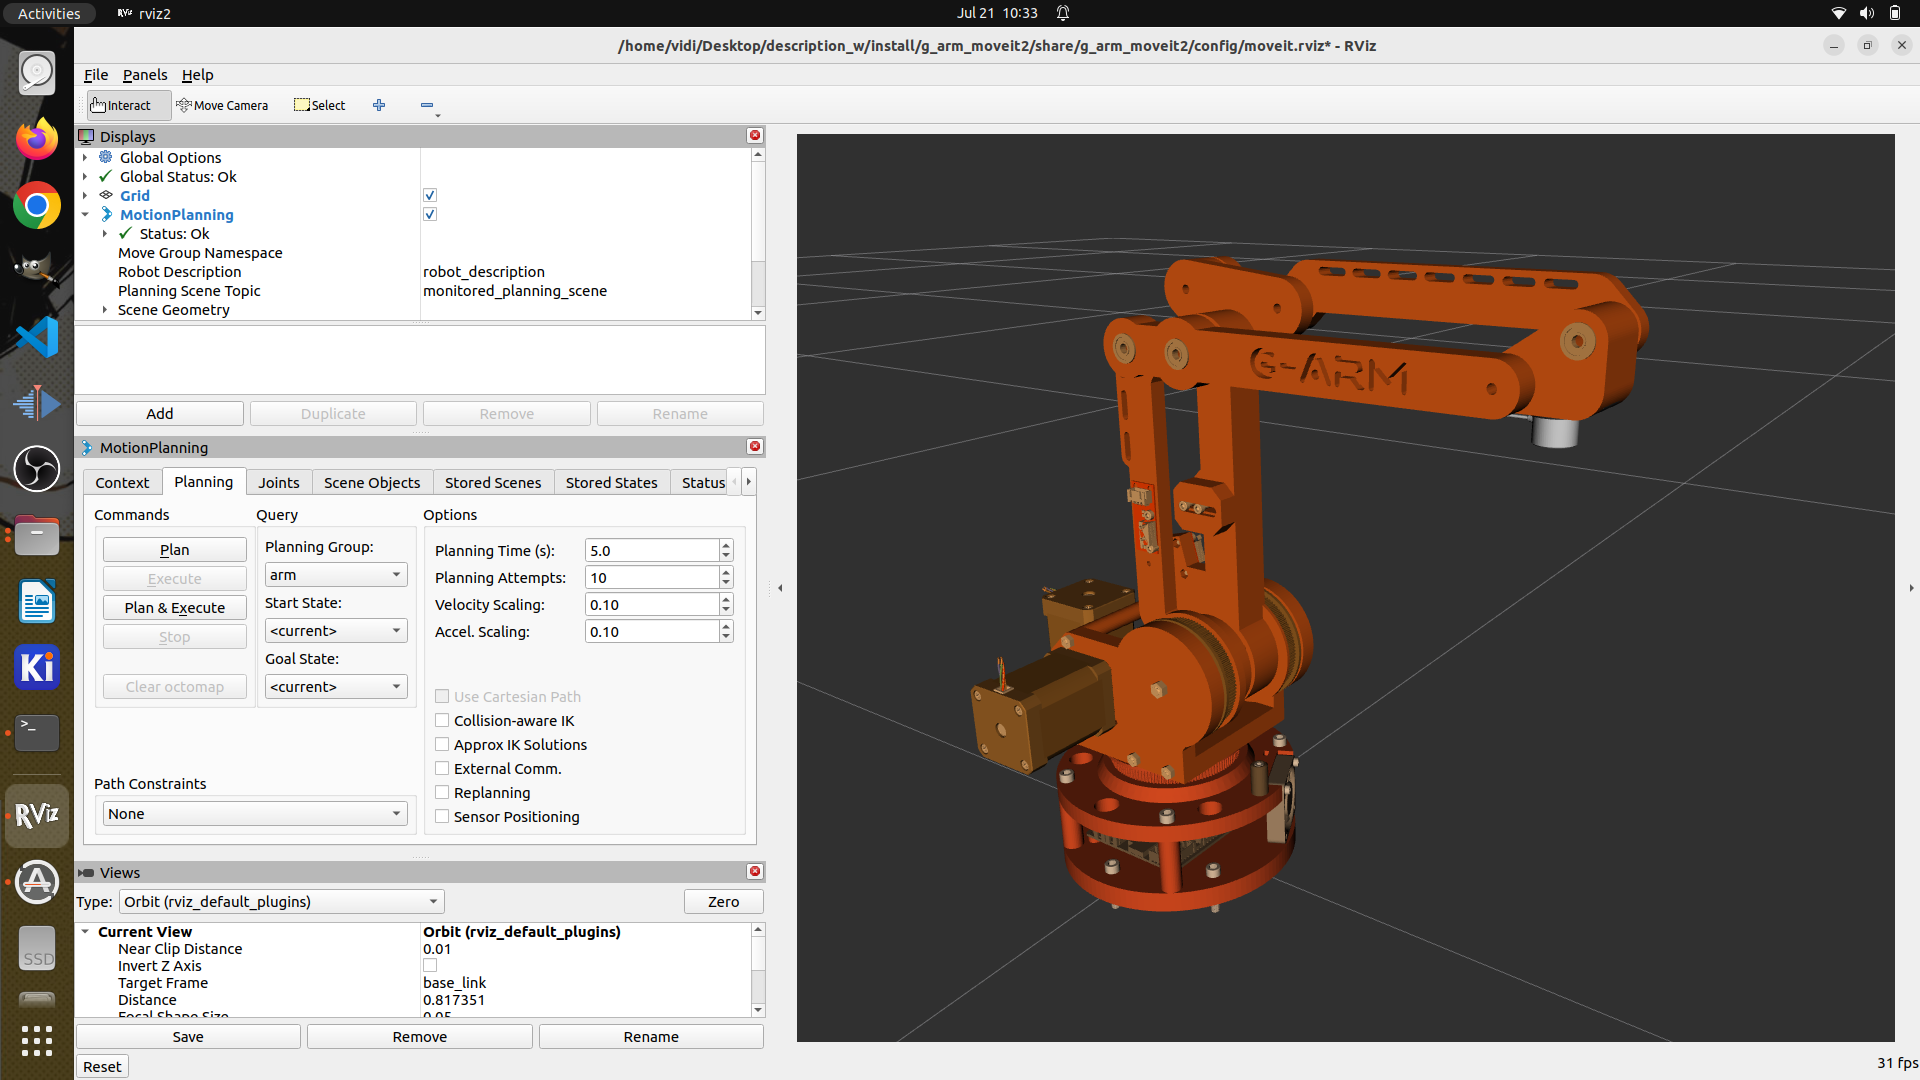
\includegraphics[width=13cm]{figs/moveit_demo.png}
    \end{center}
    \caption{Rviz al lanzar el \textit{demo.launch.py}}
    \label{fig:moveit_demo}
\end{figure}\ 

\begin{figure} [ht!]
    \begin{center}
      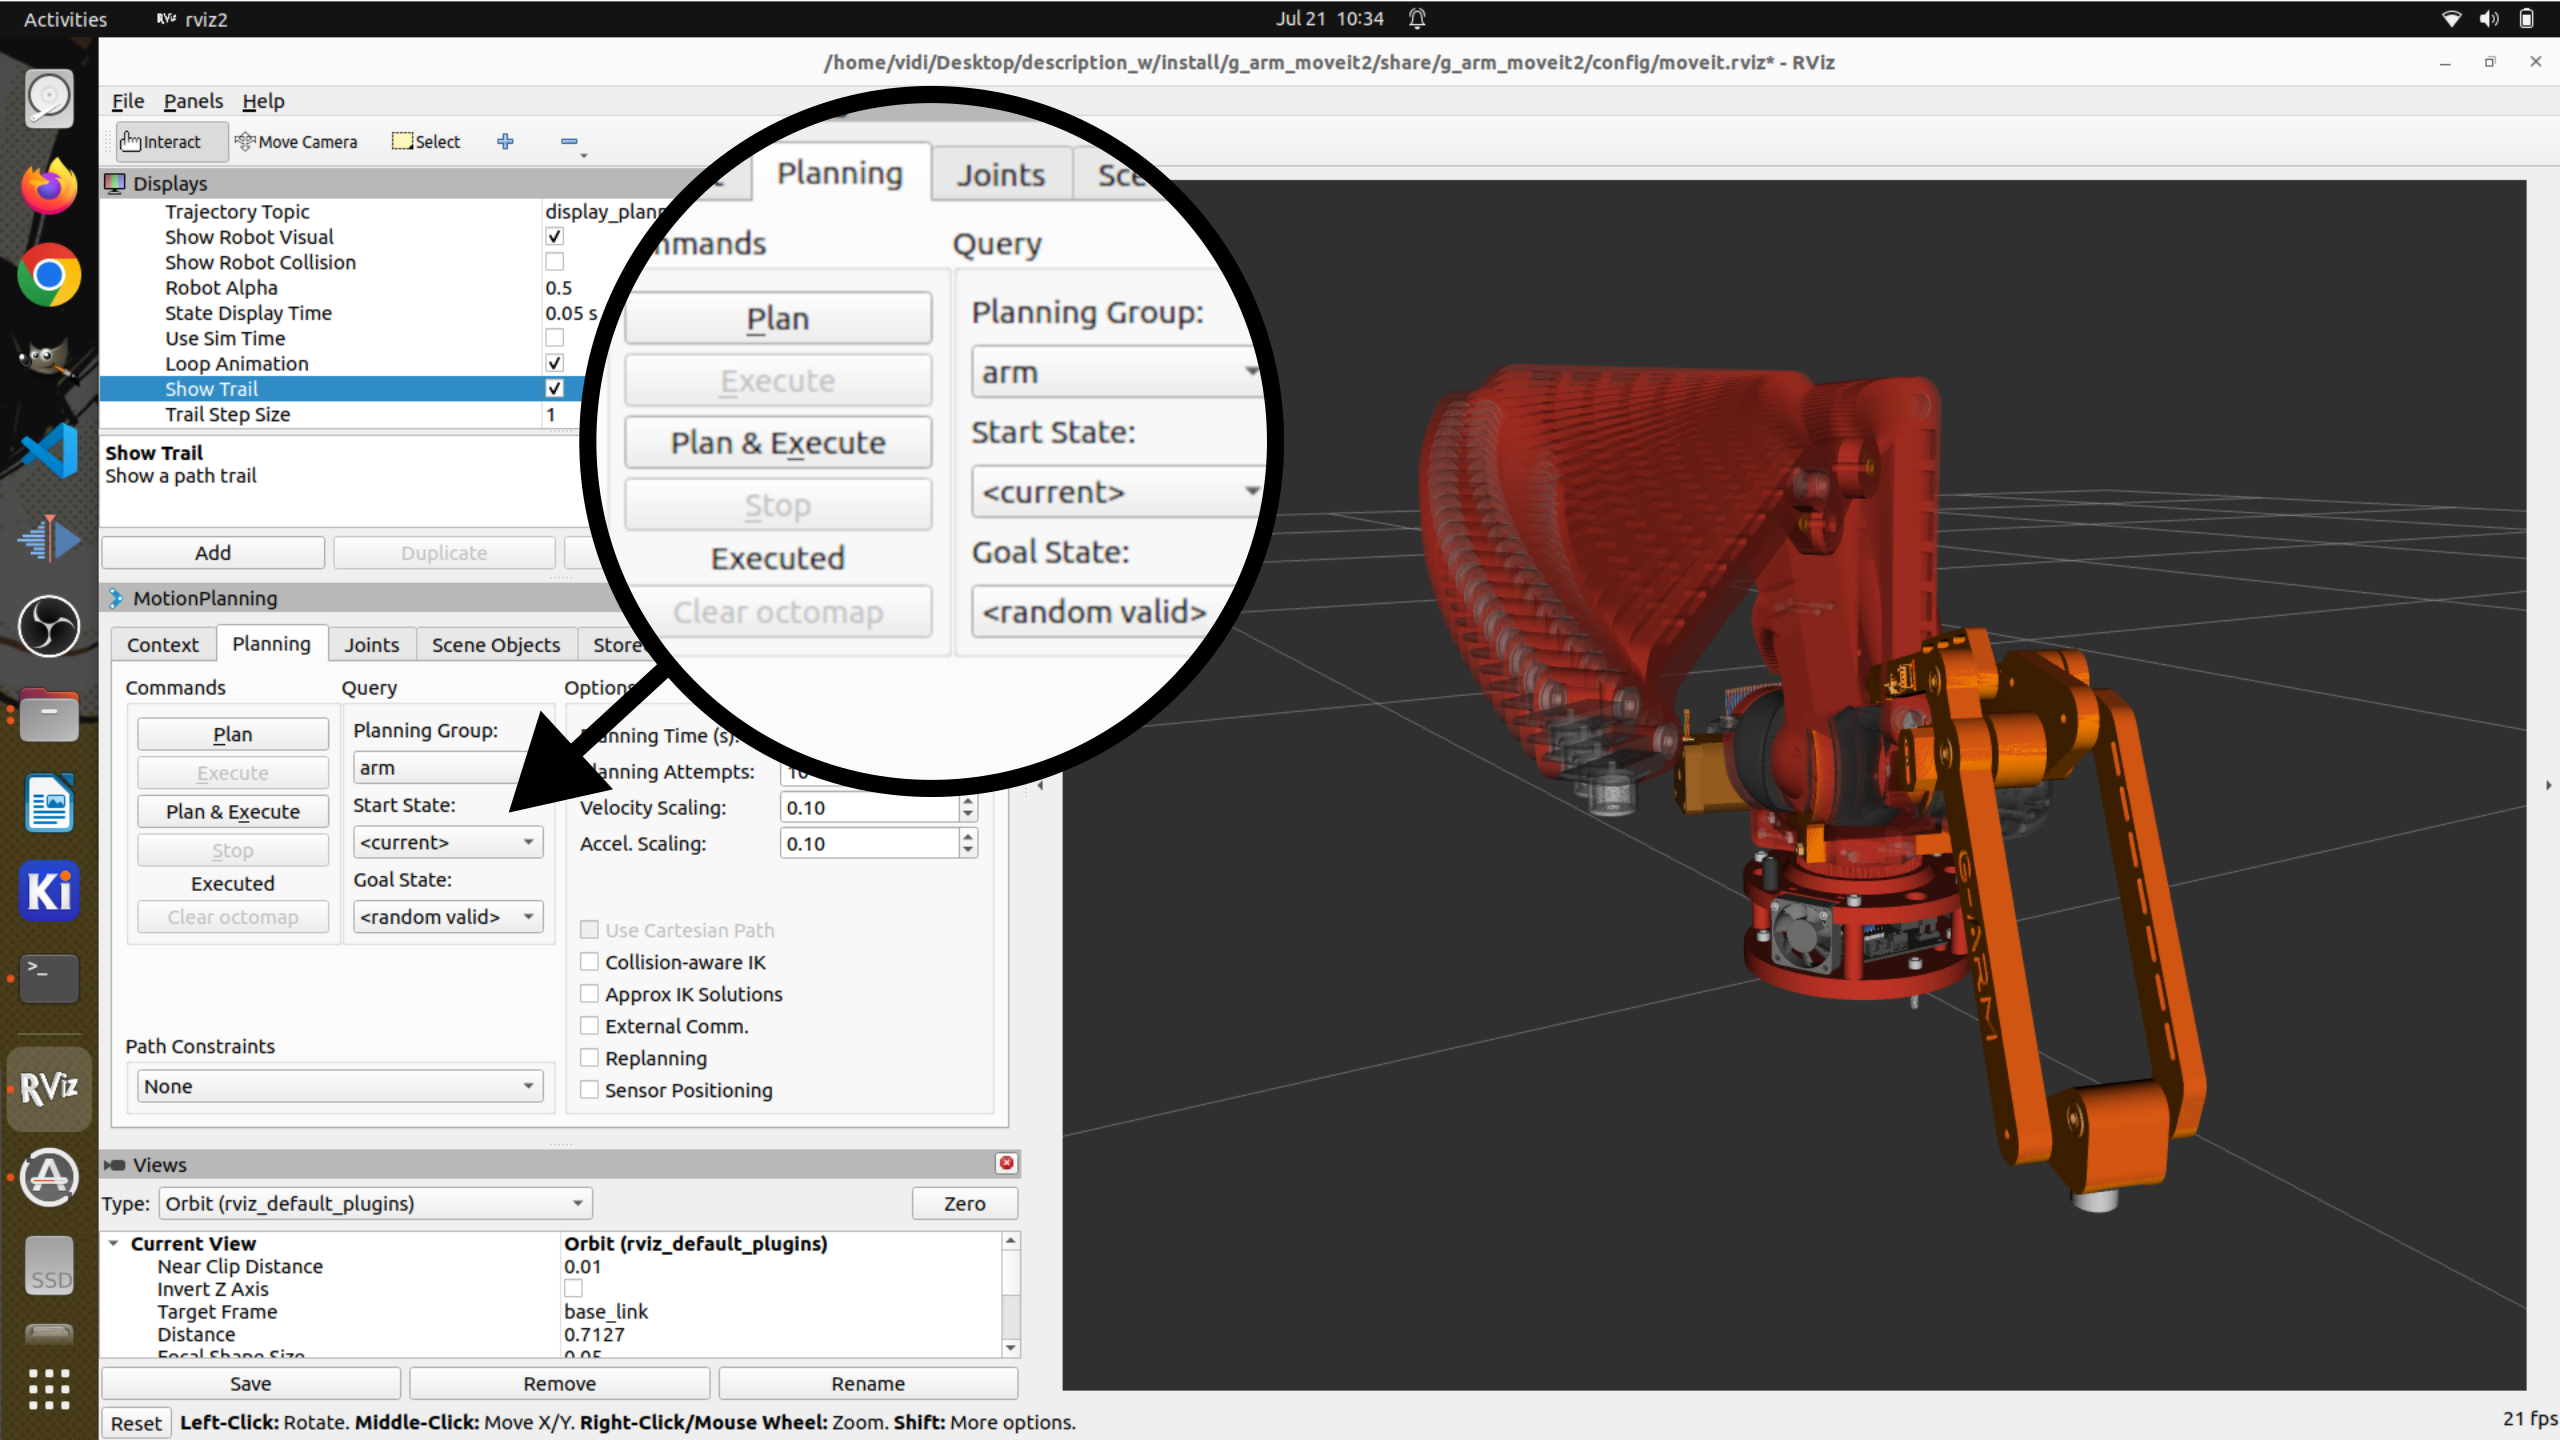
\includegraphics[width=13cm]{figs/moveit_demo_trajectory.png}
    \end{center}
    \caption{Planificando una trayectoria simple}
    \label{fig:moveit_trayectory_demo}
\end{figure}\ 

\subsection{Driver para ROS}
\noindent En esta sección se detalla el funcionamiento del nodo ROS creado para ejecutar las trayectorias en el robot real.
\\


Primeramente es necesario comprender el funcionamiento de este framework, al menos su parte más externa, aquella que 
se comunica con el exterior. 
Según la documentación\footnote{\url{https://moveit.picknik.ai/humble/doc/concepts/move_group.html}}, existe 
un nodo llamado \textit{move\_group} (Véase la Figura\ref{fig:arquitectura_moveit}) que se comunica con resto del framework 
a través de los topics y acciones de ROS. De cara al exterior, puede establecer conexión con dos elementos del propio entorno del robot. 
El primero es la percepción, en este caso permite obtener información de la escena a través de los datos de una cámara 3D. El segundo es el 
controlador del robot, que se encarga de aceptar y ejecutar las trayectorias requeridas, además de devolver información acerca del 
progreso.
\begin{figure} [ht!]
    \begin{center}
      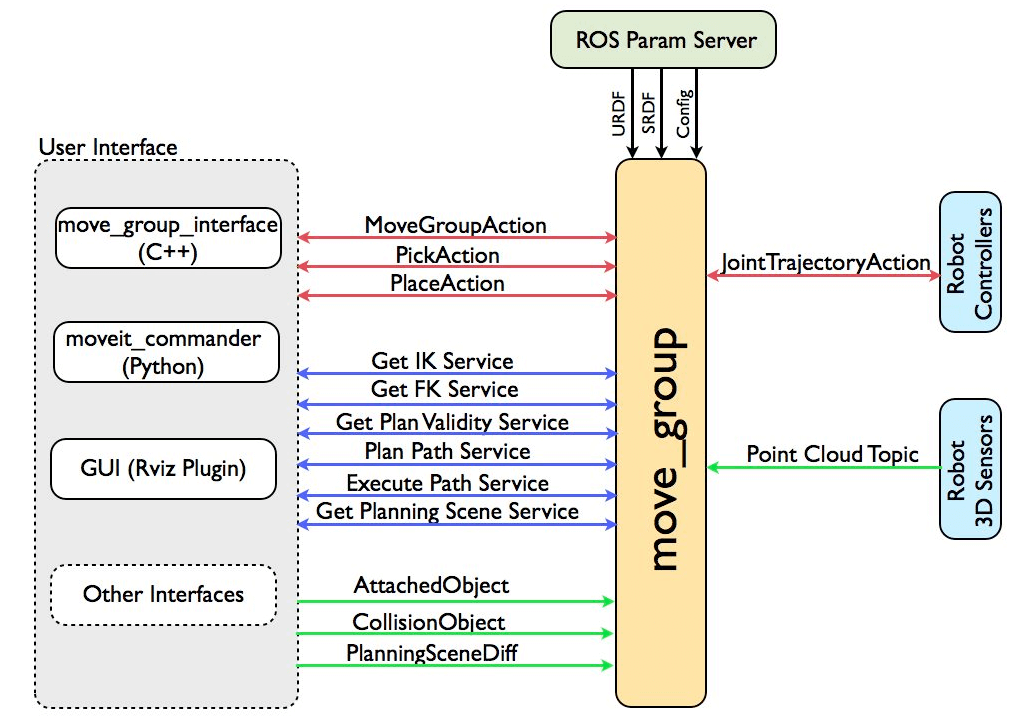
\includegraphics[width=12cm]{figs/moveit_arquitectura.png}
    \end{center}
    \caption{Relación de \textit{move\_group} con el resto del \textit{Firmware}}
    \label{fig:arquitectura_moveit}
\end{figure}\ 
\newpage
Según la propia documentación, la forma más simple y eficaz de controlar el robot real es utilizando un controlador de 
\mbox{\textit{ros2\_control}\footnote{\url{https://control.ros.org/master/index.html}}}
e imitar en el robot real las posiciones de los distintos joints publicadas por el controlador. En sí \mbox{\textit{ros2\_control}} es un 
framework que incorpora una gran cantidad de herramientas para implementar sistemas de control en ROS. Dentro de él, existen los llamados 
controladores y según su tipo pueden controlar robots de tracción diferencial, direcciones Ackermann, entre otros. Para esta aplicación el que nos 
interesa es \mbox{\textit{Joint Trajectory Controller}}, un controlador diseñado para ejecutar trayectorias en el espacio de 
articulaciones, interpolando entre uno o más puntos de referencia. Conjuntamente con esto, hay que 
utilizar otro nodo llamado \textit{joint\_state\_broadcaster}, que lee las interfaces de estado del controlador y las publica en los topics
\textit{/dynamic\_joint\_states} y \textit{/joint\_states}. Siendo finalmente este último topic el que deberá ser escuchado por el 
nodo del robot real para extraer la posición 
de cada articulación. En el Bloque de código \ref{cod:campos} se muestran los campos del mensaje enviado a través 
de él.
\lstset{language=C++,
        basicstyle=\ttfamily,
        keywordstyle=\color{blue},
        commentstyle=\color{green},
        stringstyle=\color{orange},
        showstringspaces=false,
        breaklines=true,
        breakatwhitespace=true}

\begin{code}[h]
\begin{lstlisting}
Header header

string[] name
float64[] position
float64[] velocity
float64[] effort
\end{lstlisting}
\caption{Campos del tipo de mensaje \mbox{\textit{sensor\_msgs/msg/JointState}}}
\label{cod:campos}
\end{code}

El driver creado, hace uso de una clase intermedia entre el nodo ROS y la clase \textit{grbl} con el fin de abstraer al nodo de la conversión 
de unidades. Además, esta nueva clase incorpora lo necesario para encontrar los límites físicos de cada articulación sumado a una serie de 
constantes usadas para hacer que la posición absoluta de las articulaciones concuerde con la usada en la descripción del robot. \\

Al comenzar, trata 
de conectarse al robot y busca el 0,0 de cada joint. Posteriormente crea una subscripción al topic \textit{/joint\_states} para recibir y 
guardar el último mensaje que llega a través de  este topic. En paralelo a esto, existe una función llamada con una cierta frecuencia (utilizando un 
\textit{timer} de ROS) que envía las posiciones del mensaje, previamente guardado, al robot real. Se ha decidido separar ambos comportamientos 
para tener un cierto control sobre la frecuencia de envíos de datos por el puerto serie y evitar saturar el firmware del robot. 
\newpage
En la Figura \ref{fig:dia_driver1} se muestra el diagrama de actividades que ilustra el funcionamiento básico del driver creado.\\
\\


\begin{figure} [ht!]
    \begin{center}
      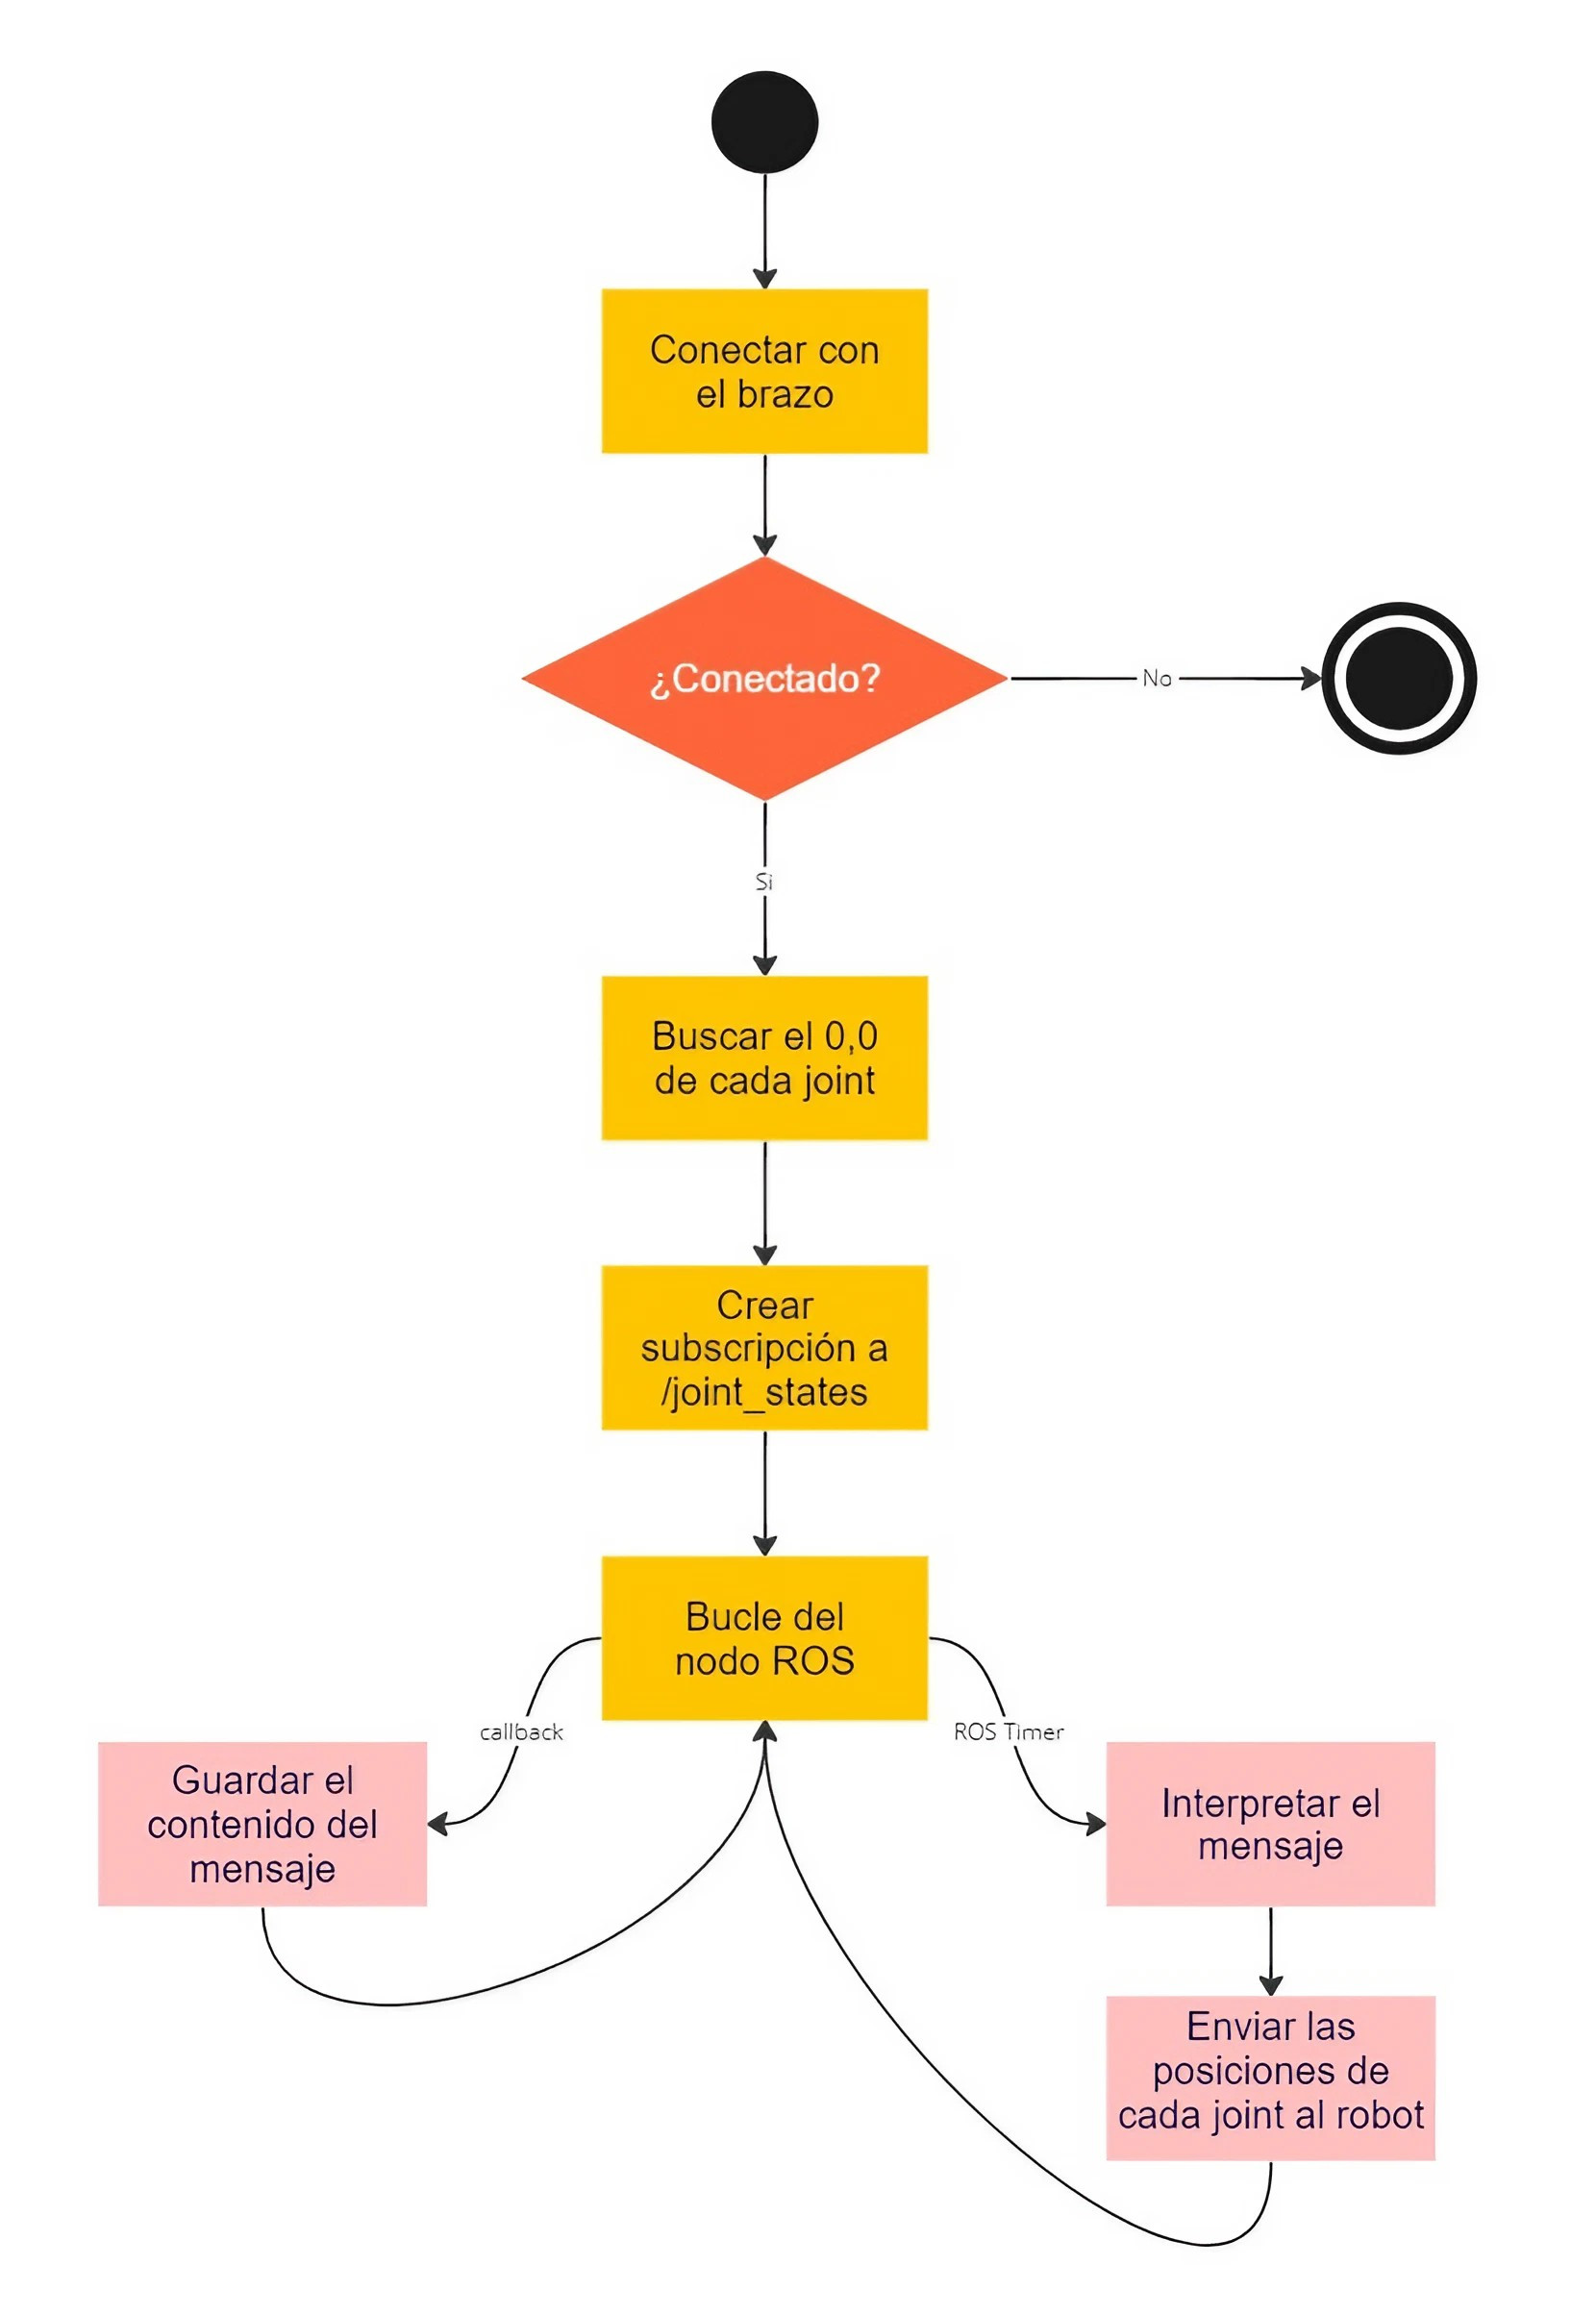
\includegraphics[width=11cm]{figs/driver_diagram1.jpg}
    \end{center}
    \caption{Diagrama de actividades del driver}
    \label{fig:dia_driver1}
\end{figure}\ 


Por suerte, el propio lanzador de demostración mencionado en la sección anterior, ya levanta estos nodos por lo que no es necesario crear 
uno nuevo para realizar las pruebas. Más adelante sí es recomendable hacerlo, para poder tener mayor control sobre los nodos 
que se están lanzando y añadir nuevos si es necesario.
\\

\newpage
\section{Pruebas}
\noindent En esta sección se ponen a prueba los aspectos técnicos que determinan el desempeño y la fiabilidad del brazo robot. Para ello, 
se han llevado a cabo una serie de pruebas, bajo distintas circunstancias, y se han apuntado los resultados.
\subsection{Capacidad de carga}
\noindent En este apartado se pone a prueba la capacidad del robot a la hora de levantar y mover cargas con diferentes masas. 
Para ello, se han considerado los siguientes escenarios:
\begin{itemize}
    \item Escenario 1: El robot comienza con el brazo completamente extendido y empieza a levantar lentamente distintas cargas. La 
    prueba finaliza cuando los motores no son capaces de soportarlo.
    \item Escenario 2: Repetir el escenario 1 pero situando la carga cerca de la base.
    \item Escenario 3: El robot hace uso de su herramienta electroimán (teóricamente de 3Kg de fuerza) para levantar distintas cargas unidas a un 
    objeto ferromagnético. La prueba finaliza cuando el electroimán no es capaz de sujetar la carga o bien, el robot no es capaz de levantarla.
\end{itemize}

\begin{figure} [ht!]
    \centering  
    \subfigure[Escenario 1]{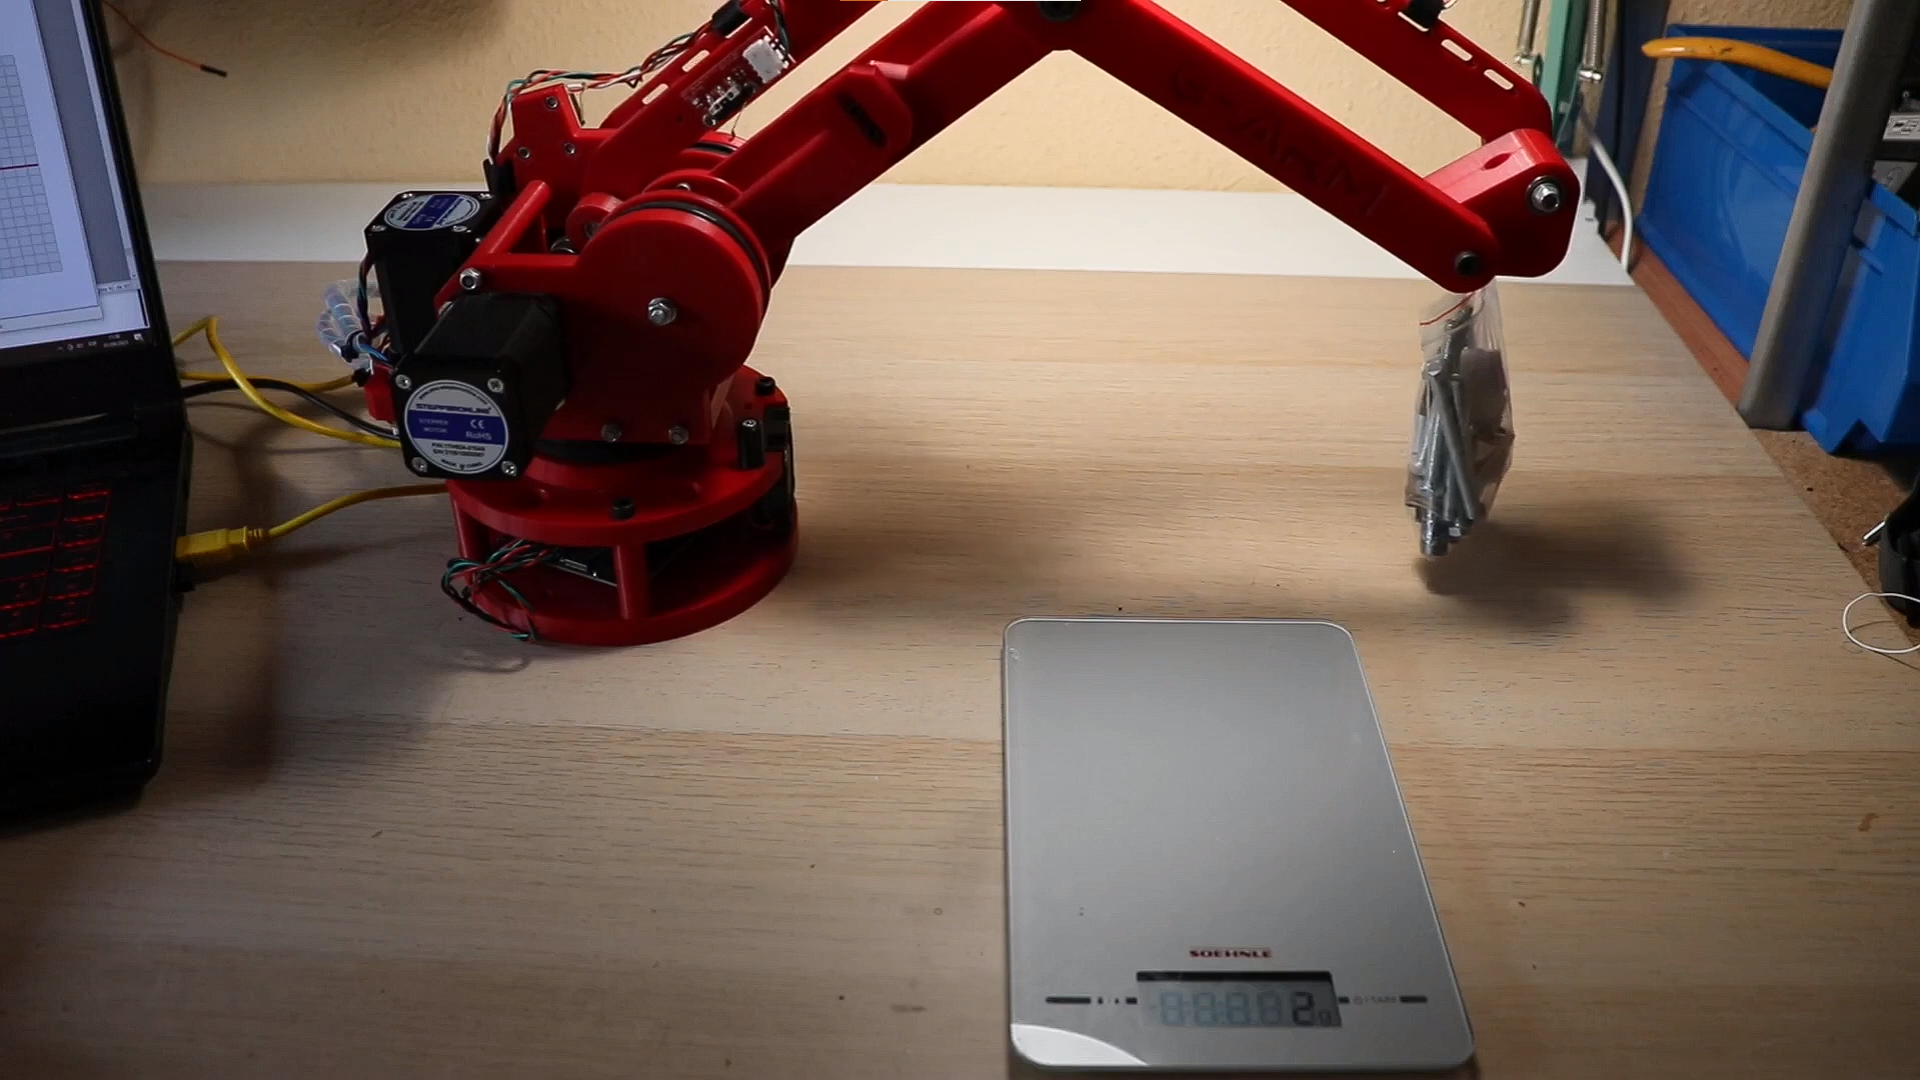
\includegraphics[width=0.3\linewidth ]{figs/loadTest1.png}}
    \hspace{2cm}
    \subfigure[Escenario 2]{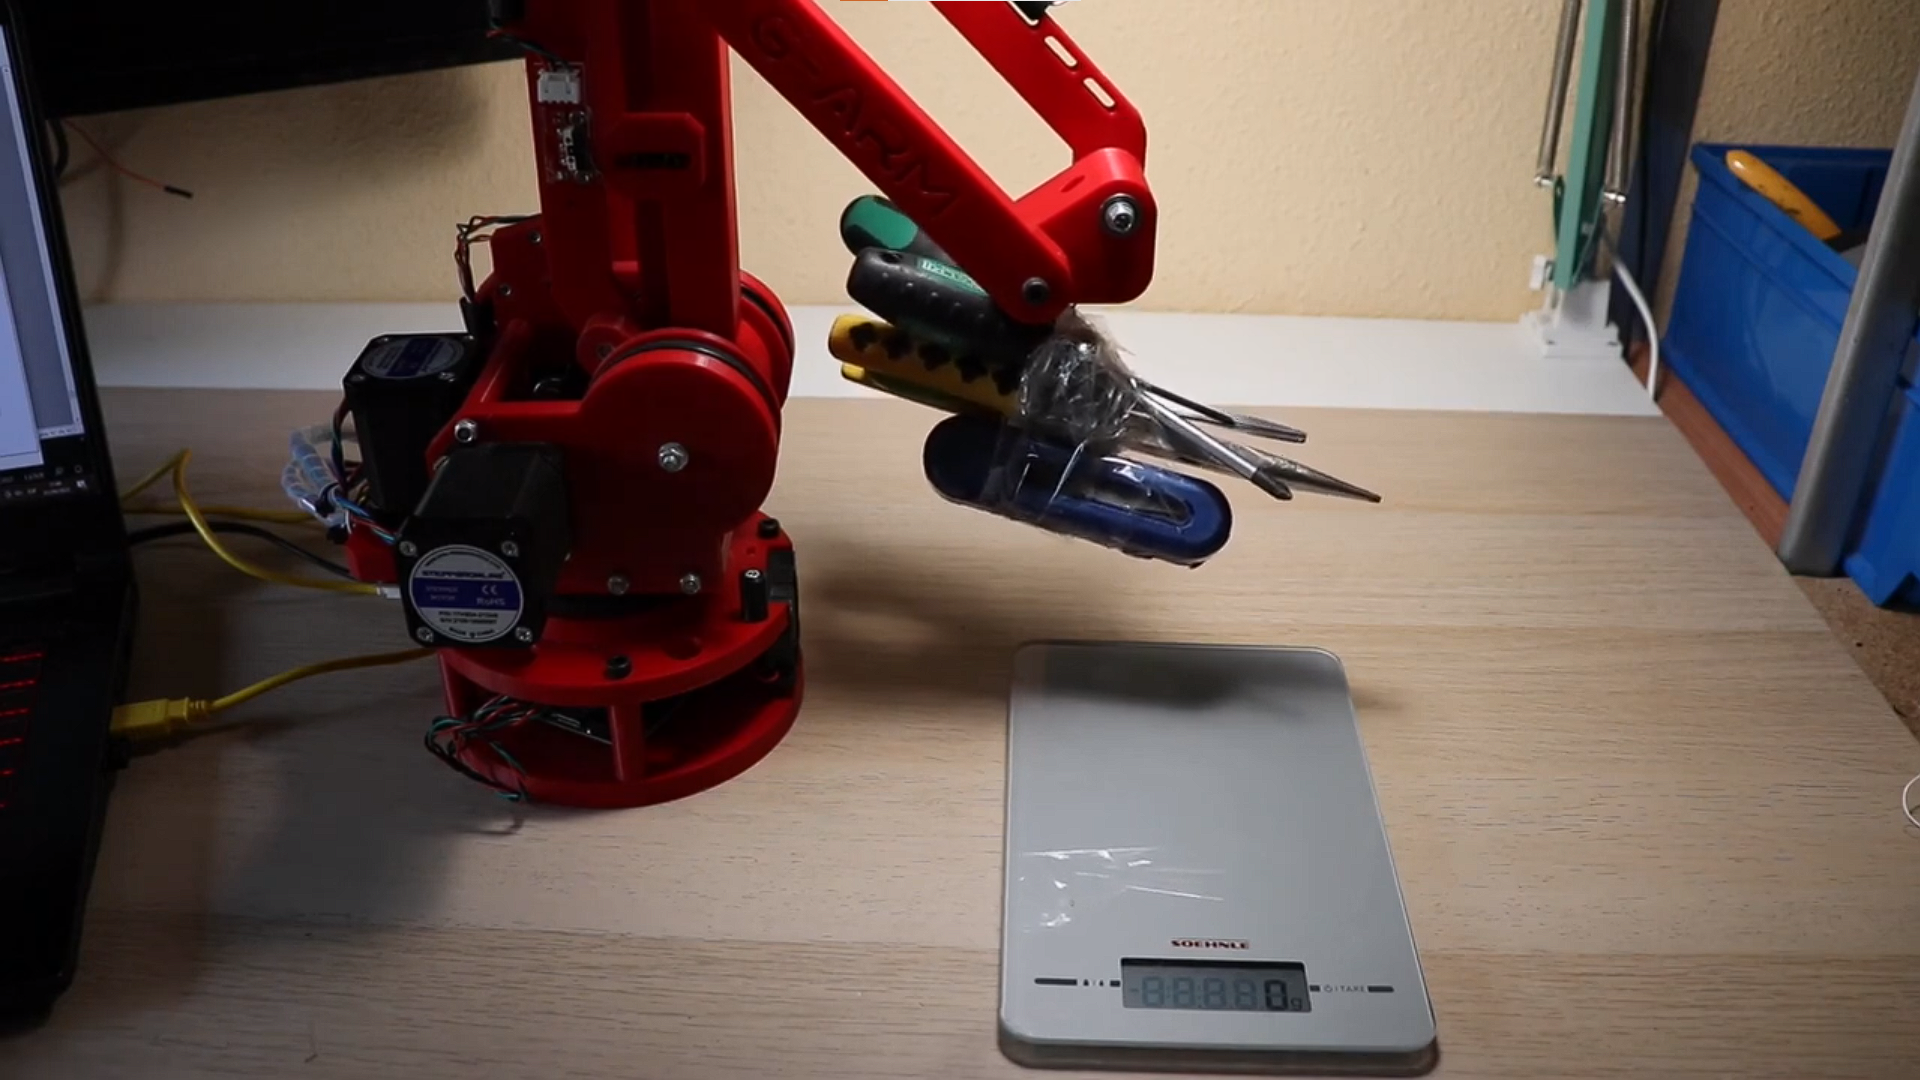
\includegraphics[width=0.3\linewidth ]{figs/loadTest2.png}}
    \hspace{2cm}
    \subfigure[Escenario 3]{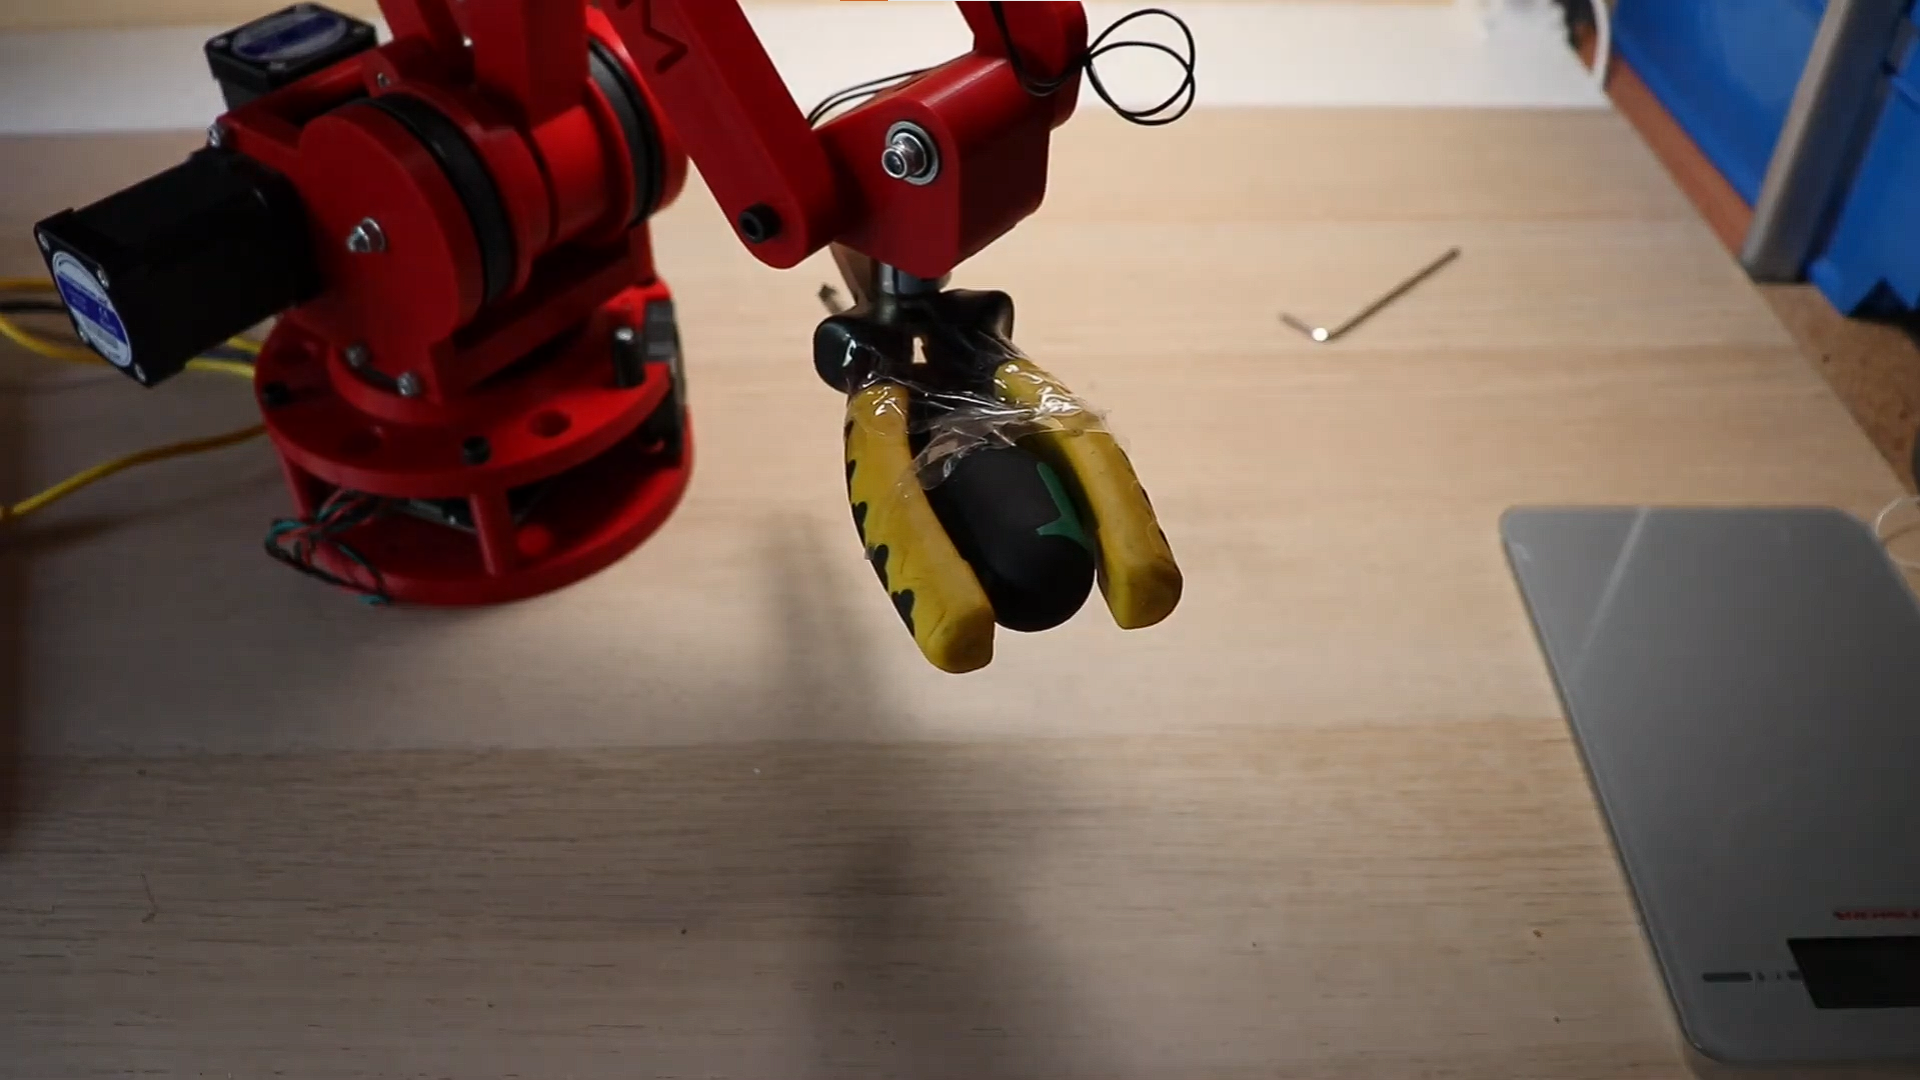
\includegraphics[width=0.3\linewidth ]{figs/loadTest3.png}}
    \caption{Fotos extraídas del vídeo de las pruebas de carga\footnote{\url{https://youtu.be/McD7kLMKMo0}}}
    \label{fig:loadTests}
\end{figure}\ 

Los resultados obtenidos se muestran en el Cuadro \ref{cuadro:evaluacion_carga}. De esta prueba podemos extraer que 
el brazo es capaz de levantar una carga significativa a pesar de su reducido tamaño. También, se ha comprobado que el 
electroimán que se anunciaba como capaz de sostener 3 KG, sólamente es capaz de levantar una décima parte de ello. A pesar de esto, es capaz de levantar y manipular tornillos y objetos metálicos pequeños, incluso en 
movimientos rápidos. Más allá de los valores de carga máximos, el comportamiento del robot durante la prueba 
hace pensar que es capaz de manejar cargas de hasta 150g con total normalidad. A modo de ejemplo, en la siguiente prueba se monta un mando 
de televisión de 100g y se realizan movimientos rápidos con él.

\begin{table}[H]
\begin{center}
\begin{tabular}{|c|c|}
\hline
\textbf{Escenario} & \textbf{Carga máxima} \\
\hline
Escenario 1& \SI{365}{\gram} \\
Escenario 2 & \SI{480}{\gram} \\
Escenario 3 & \SI{305}{\gram} \\
\hline
\end{tabular}
\caption{Resultados de los diferentes resultados en la prueba de carga}
\label{cuadro:evaluacion_carga}
\end{center}
\end{table}

\subsection{Velocidad máxima}
\noindent En esta prueba se evalúa que tan rápido se puede mover cada articulación con una carga de 100g. Para realizar esta prueba  
se han configurado unas aceleraciones más altas de lo normal y se le ordena moverse a una velocidad inalcanzable. En esta prueba, 
el robot permanece unido a la mesa mediante unos sargentos para evitar que la inercia haga deslizar la base. Se ha utilizado 
la línea de tiempo del vídeo para saber en que segundo y décima de segundo se comienza a mover el robot y en qué momento 
exacto llega a su destino. Se ha establecido un rango conocido de grados para poder hallar una velocidad media en ese tramo. 
En el pie de página se puede encontrar un enlace al vídeo de la prueba realizada, donde se ve la velocidad que es capaz de 
alcanzar este brazo. En la Figura \ref{fig:speedTests} se pueden ver algunas imágenes extraídas del propio vídeo.
\begin{figure} [ht!]
\centering  
\subfigure[Inicio del recorrido]{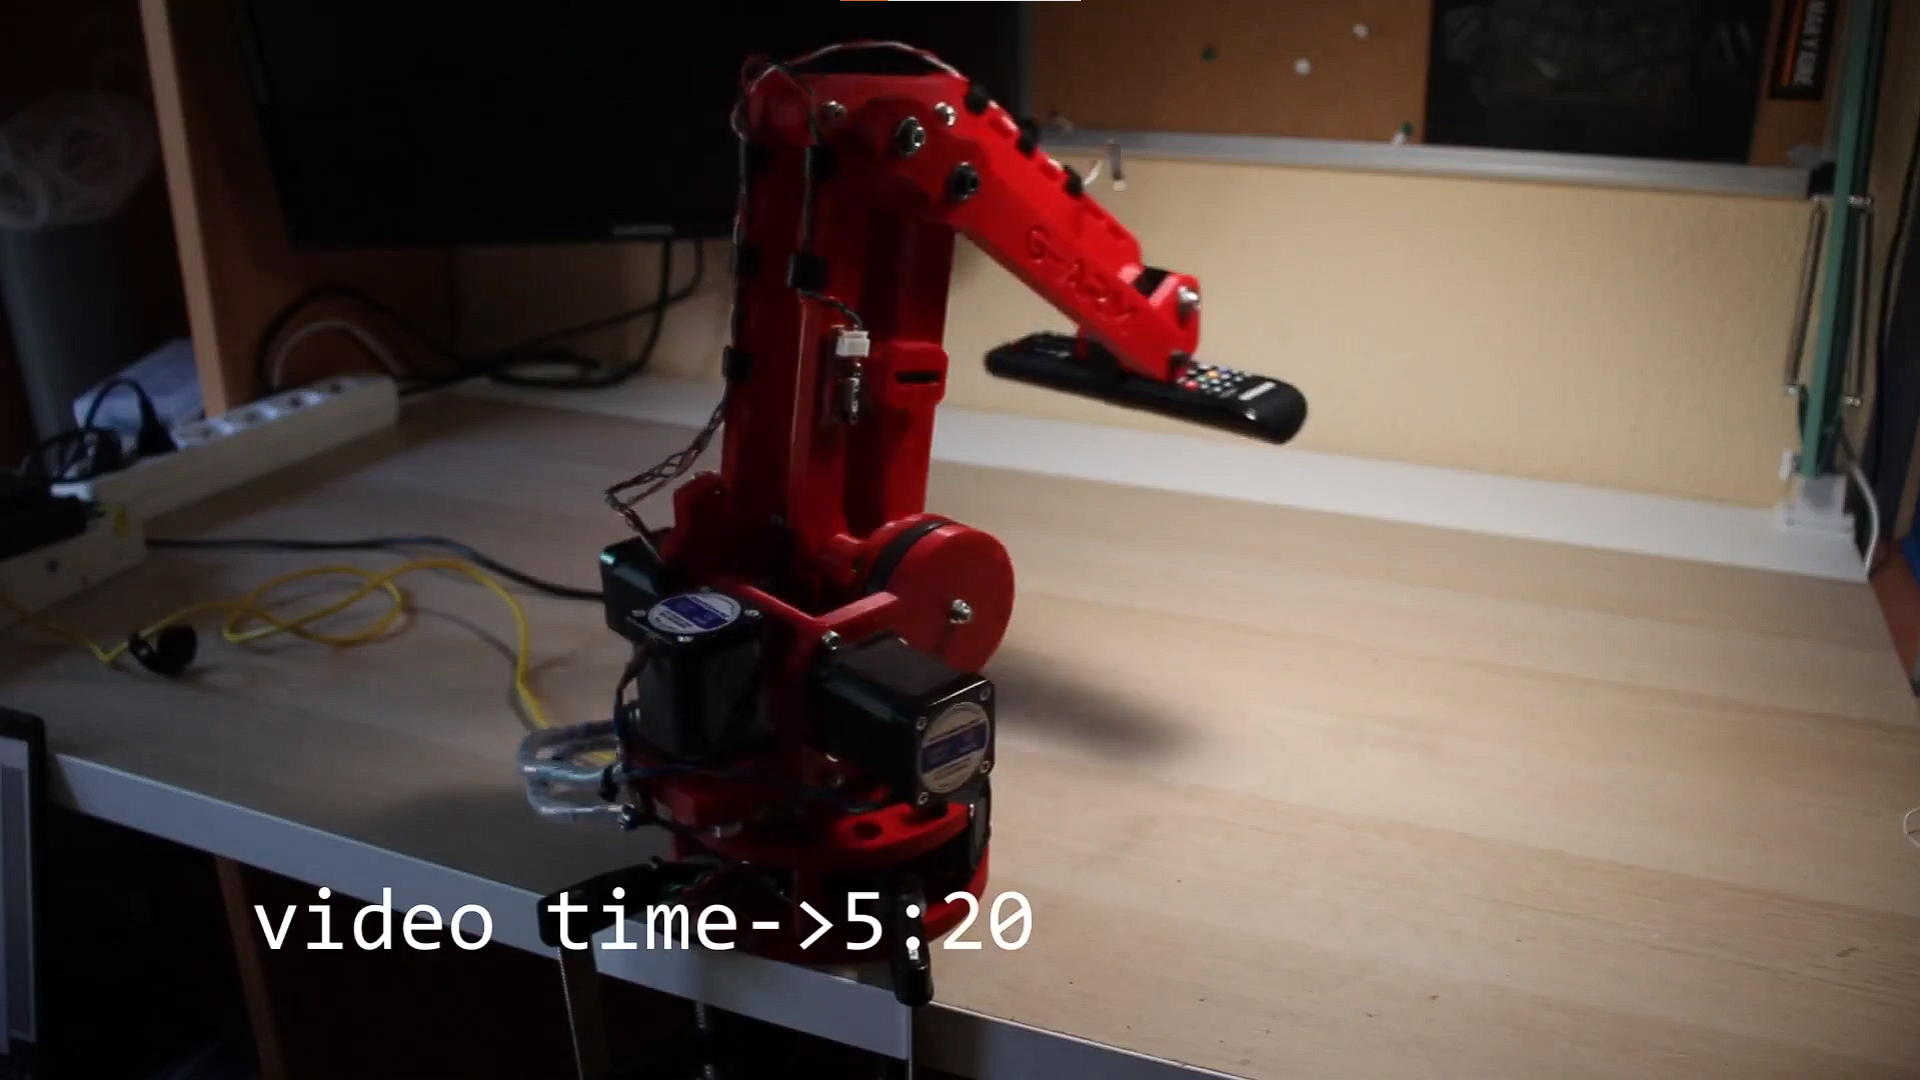
\includegraphics[width=0.45\linewidth ]{figs/speedTest1.png}}
\hspace{1cm}
\subfigure[Final del recorrido]{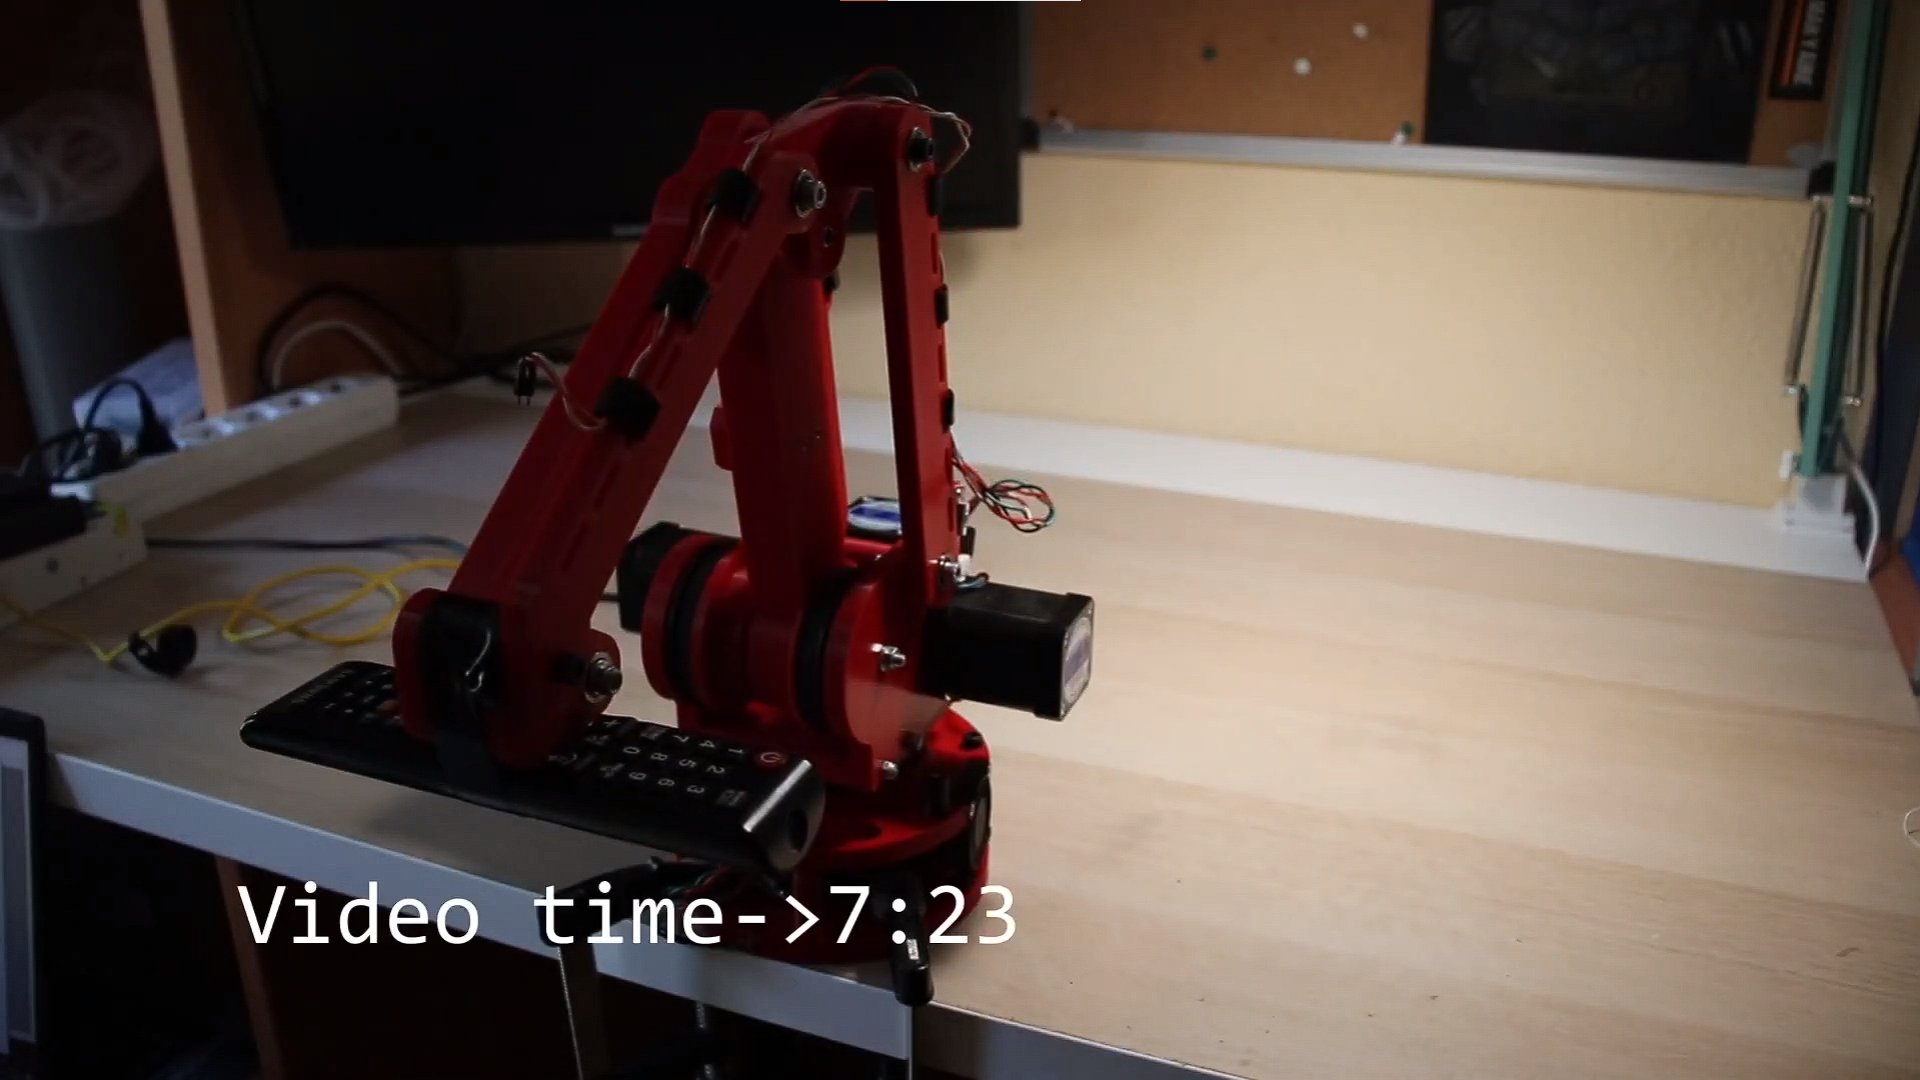
\includegraphics[width=0.45\linewidth ]{figs/speedTest2.png}}
\caption{Fotos extraídas del vídeo de las pruebas de velocidad\footnote{\url{https://youtu.be/37KK_hJk_tI}}}
\label{fig:speedTests}
\end{figure}\ 
\newpage
Como resultado, se ha llegado a la conclusión que la velocidad máxima de giro de la articulación de la base es de 225 grados 
por segundo. Aún así la velocidad media ha sido de 90º/s debido a que primero tiene que acelerar hasta alcanzar la velocidad 
máxima y despúes frenar. Este eje ha hecho un recorrido de 180 grados en a penas 2 segundos. En ese tramo es capaz de alcanzar 
la velocidad máxima durante al menos 90 grados. Esta es una velocidad increíble teniendo en cuenta que la velocidad 
máxima de la base de un robot ABB IRB120 es de 250º/s. En cuanto a las otras dos articulaciones, al tener recorridos menores 
se consigue una máxima de 120º/s. 

\subsection{Consumo eléctrico} 
\label{sec:consumo}
\noindent Este tipo de pruebas evalúan cuanta energía está consumiendo el robot bajo unas condiciones concretas. Es útil para 
conocer el coste de tener en funcionamiento este robot y si es viable utilizarlo sobre plataformas móviles a baterías. 
\\
Para realizar este test, se han considerado 3 escenarios:
\begin{itemize}
\item Escenario 1: El robot realiza movimientos lentos.
\item Escenario 2: El robot realiza movimientos rápidos
\item Escenario 3: El robot se encuentra bloqueado en una posición fija.

\begin{figure} [ht!]
    \centering  
    \subfigure[Multímetro en serie]{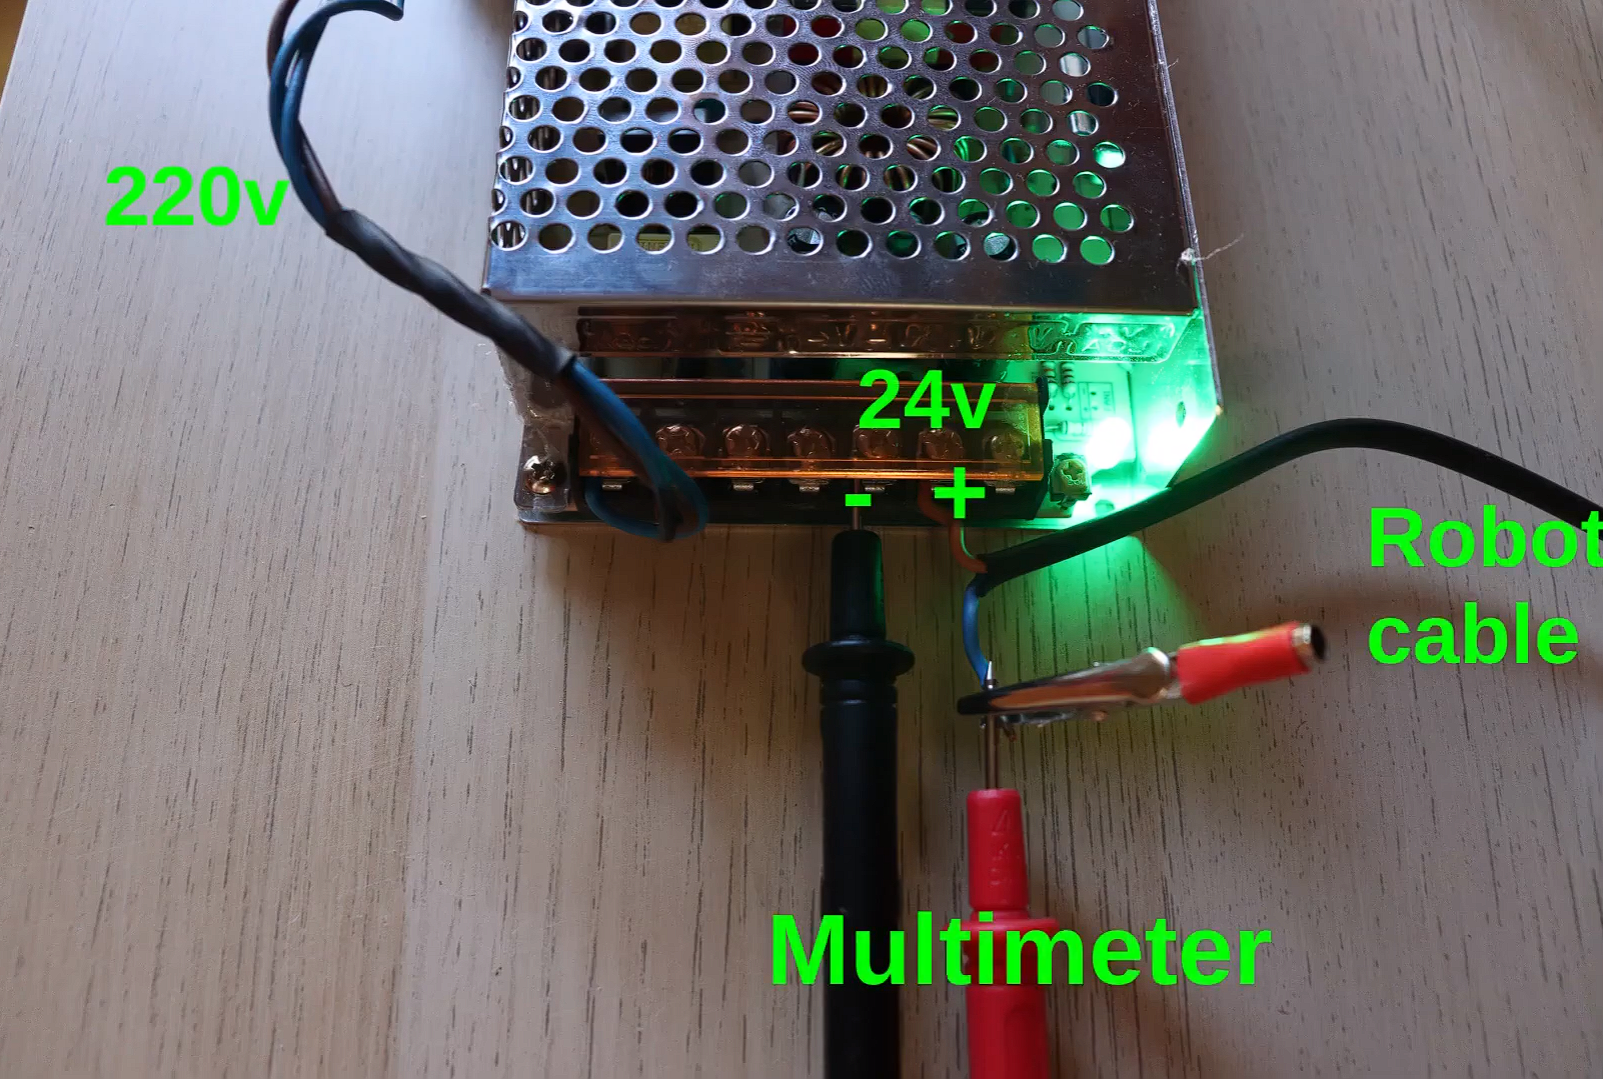
\includegraphics[width=0.4\linewidth ]{figs/powerTest1.png}}
    \hspace{1cm}
    \subfigure[Escenario de la prueba]{\includegraphics[width=0.45\linewidth ]{figs/powerTest2.png}}
    \caption{Fotos extraídas del vídeo de las pruebas de consumo\footnote{\url{https://youtu.be/2MfBabEWZNo}}}
    \label{fig:powerTests}
\end{figure}\ 

\end{itemize}
\indent Los resultados obtenidos estan recogidos en el Cuadro \ref{cuadro:consumos}. Como se puede observar, realmente no existe una gran 
diferencia entre un movimiento rápido y uno lento, en cambio, la diferencia sí es notable cuando lo comparamos con permanecer en 
una posición fija. Hay que recordar que aunque esté en parado, las bobinas de los motores permanecen excitadas para 
mantener su posición. 

Gracias a esta prueba, queda comprobado que sí puede ser usado sobre plataformas móviles y ser 
alimentado mediante baterías. De hecho, es ideal para ser montado sobre un robot Turtlebot 2 utilizando la salida de 19V o 12V que incorpora 
en su base.
\begin{table}[H]
\begin{center}
\begin{tabular}{|c|c|}
\hline
\textbf{Escenario} & \textbf{Consumo medio}\\
\hline
Escenario 1 & 14.4W\\\
Escenario 2 & 17W\\
Escenario 3 & 6.8W\\
\hline
\end{tabular}
\caption{Consumos eléctricos en distintos escenarios}
\label{cuadro:consumos}
\end{center}
\end{table}


\chapter{Conclusiones}
\label{cap:capitulo7}

\begin{flushright}
\begin{minipage}[]{10cm}
\emph{Quizás algún fragmento de libro inspirador...}\\
\end{minipage}\\

Autor, \textit{Título}\\
\end{flushright}

\vspace{1cm}

En el último capítulo, se hará mención a los logros alcanzados en términos de objetivos y se presentarán 
las conclusiones obtenidas en este proyecto. También se discutirán las habilidades y conocimientos 
adquiridos durante su desarrollo, así como las posibles mejoras futuras a tener en cuenta.
\section{Objetivos cumplidos}
Primeramente cabe destacar que se ha logrado cumplir el objetivo principal de este trabajo:
Enumera los objetivos y cómo los has cumplido.\\

Enumera también los requisitos implícitos en la consecución de esos objetivos, y cómo se han satisfecho.\\
\section{Competencias adquiridas}
En el desarrollo de este trabajo se han adquirido una gran cantidad de conocimientos y competencias y conocimientos, 
entre los cuales destacan:
\begin{itemize}
\item Conocimientos avanzados acerca de Grbl y su funcionamiento más interno.
\item Se ha adquirido una amplia soltura en el manejo de la herramienta de diseño FreeCad y en multitud de sus bancos de trabajo (Draft, A2Plus, Fasteners, Mesh...).
\item Se ha ganado una gran experiencia en el diseño de piezas mecánicas para su posterior impresión en 3D.
\item Aumento en la capacidad de planificación de tareas y organización de los recursos disponibles.
\item Manejo más rápido y descubrimiento de comandos nuevos de la herramienta Git.
\item Ampliación de conocimientos en ROS 2 y dominio pleno del formato URDF (particularidades, limitaciones y puntos fuertes).
\item Conocimiento del funcionamiento interno del framework MoveIt y la configuración de paquetes para usarse dentro de él.
\item Generar documentación de calidad para un trabajo y comprender la documentación de otros proyectos para poder 
utilizarlos posteriormente en proyectos propios.
\item Conocimientos avanzados en electrónica y en sistemas relacionados con el mundo de las máquinas CNC.
\item Gran dominio de los parámetros de impresión, para lograr piezas con las tolerancias correctas y un acabado visual perfecto. 
\end{itemize}

Por último, añade otro par de párrafos de líneas futuras; esto es, cómo se puede continuar tu trabajo para abarcar una solución más amplia, o qué otras ramas de la investigación podrían seguirse partiendo de este trabajo, o cómo se podría mejorar para conseguir una aplicación real de este desarrollo (si es que no se ha llegado a conseguir).
\section{Valoración final y líneas futuras}
Se ha desarrollado un robot eficaz y barato capaz de cumplir con su cometido de poder usarse en la docencia universitaria. Es por esto 
que se plantean las siguientes líneas futuras para continuar con el proyecto y mejorarlo todavía más:

\begin{itemize}
    \item Añadir un cuarto grado de libertad en el extremo del robot para poder rotar objetos en el plano de trabajo.
    \item Utilizar un rodamiento de mayor tamaño en la rotación de la base para reducir la flexión del robot al estar sometido 
    a cargas pesadas.
    \item Crear una serie de herramientas nuevas para acoplar a este robot como puede ser un porta rotulador, una pinza o un láser.
\end{itemize}




\clearpage
\thispagestyle{empty}

\printindex \nocite{*}
\appendix
\bibliographystyle{apalike} \bibliography{bibliografia}

\end{document}
